\documentclass[10pt]{memoir}
\usepackage{amsmath,amsfonts,amssymb,amsthm}
%\usepackage[tight]{diagrams}
\usepackage{MnSymbol}
\usepackage[mathlf,textlf,minionint]{MinionPro}
\DeclareMathSymbol{\mycomplement}   {\mathord}{AMSa}{"7B}
%\usepackage[T1]{fontenc}
%\usepackage{textcomp}
\usepackage{calc,url}
\usepackage{algpseudocode}
\usepackage{algorithmicx}
\usepackage[pdftex]{color,graphicx}
\usepackage{lecmath,lecmemoir,lecpagesize}
\theoremstyle{mybem}
\usepackage{exercise}
\usepackage{makeidx}
\usepackage{hyperref}
\hypersetup{colorlinks=true, unicode=true, linkcolor=[rgb]{0.10,0.05,0.67}, citecolor=[rgb]{0.10,0.05,0.67}, filecolor=[rgb]{0.10,0.05,0.67}, urlcolor=[rgb]{0.10,0.05,0.67}}
\usepackage[pdftex]{accsupp}
%\usepackage{accessibility}
%\usepackage[accsupp]{axessibility}

\let\cal=\mathcal
\def\qed{\hfill{$\square$}}

\def\mynote#1{\footnote{#1}}
\def\person#1{#1}
\def\figuref#1{Figure~\ref{#1}}
\def\pointer#1{{\color{blue}\underline{$\leadsto$~\ref{#1%
}}}}
\def\bonussection{\begin{center}\textbf{BONUSSECTION}\end{center}}

\makeindex
\title{Mathematics for Computational Science}
\author{Alexander Hulpke}
\date{Spring 2021}
\begin{document}
\chapterstyle{BlueBox}%bianchi}
\frontmatter
\thispagestyle{empty}
%\maketitle
\ \\
\vspace{1mm}
\begin{center}
{\huge\textbf{\thetitle}}
\bigskip

{\large Lecture Notes}
\bigskip

{\small MATH 180A5}
\bigskip
\bigskip

{\Large\theauthor}
\medskip

{\large\thedate}
\end{center}

\ \hspace{8cm}
\vspace{2mm}
\begin{center}
\includegraphics[width=11cm]{pic/Kandinsi_CirclesInACircle.jpg}
\end{center}
\vspace{1cm}
\vfill

\hfill Version of \today
\newpage
\thispagestyle{empty}
\begin{raggedright}
{\small
Alexander Hulpke\\
Department of Mathematics\\
Colorado State University\\
1874 Campus Delivery\\
Fort Collins, CO, 80523
}
\end{raggedright}
\vfill
\setlength\epigraphwidth{4cm}
\begin{epigraphs}
\qitem{%
\textit{Title graphics:}\\
}
{Circles in a Circle (1923)}
\textsc{Wassily Kandinsky}
\end{epigraphs}
\vspace{1cm}
\begin{raggedright}
{\small
These notes are accompanying my course MATH 180,
held Spring 2021 at Colorado State University.
\bigskip

\copyright 2021 Alexander Hulpke. Copying for personal use is permitted.
}
\end{raggedright}
\newpage
%\setlength{\cftpartnumwidth}{1.5em}
\setlength{\cftchapternumwidth}{2em}
\setlength{\cftsectionnumwidth}{2.5em}
\setlength{\cftsubsectionindent}{4em}
\tableofcontents
%\input{preface}
\mainmatter
\chapter{Sets and Logic}
\label{chsets}

\section{Sets and Elements}

The basic ``data type'' of mathematics is the \defini{set}. A set is a
collection (really just a fancy word for a container that can hold things)
of objects, which are called the \defini{elements} of the set. 
We typically use squiggly parentheses $\{\,\}$ to denote a set.
For example,
imagine we have three objects, the number 2, and two other objects we call
$a$ and $b$. Then 
\[
\{2,a,b\}
\]
is the set containing exactly these three objects. To refer to it we can give it
a name, $S=\{2,a,b\}$. 
We can now make statements about which objects are elements of this set. For
example $2$ is an element of the set, while $3$ is not. We write this in
symbols (with $\in$ reading as ``is element of'') in the form
\[
2\in S,\qquad 3\not\in S
\]
We might also say ``$2$ is in $S$'' or ``$S$ contains $2$'', meaning exactly
the same.

Sets are characterized by their membership with two sets being equal if and
only if they have the same elements.
When we describe sets
by enumerating elements it does not matter in which order we write down the
elements, nor if we write them down multiple times\mynote{Of course,
sometimes one might want to be able to describe objects with multiplicities.
We will see how to describe this below \pointer{secmultiset}}.
Thus
\[
S=\{b,1,a\}=\{a,1,a,1,b,b,a\}
\]
as sets, but 
\[
S\not=\{1,2,3\},\quad S\not=\{a,b\},\quad S\not=\{2,a,a\},\quad
S\not=\{1,2,a,b\}.
\]

\subsection{Describing Sets}

In many cases, describing a set by enumerating all its elements is
hard or impossible. Thus two other techniques that are used. The first of
these is continuation with
$\ldots$ to indicate a pattern to be continued. For example, we might write
\[
E=\{\ldots,-4,-2,0,2,4,6,8,10,\ldots\}
\]
to describe the set of even integers. Similarly
$R=\{5,6,\ldots,10\}$ would describe the integers from $5$ to $10$, that is
$R=\{5,6,7,8,9,10\}$. The drawback of this method is that it relies on the
reader making the correct assumptions about the rule used to extend the
listed numbers. It thus -- and this is the second method -- is often easier
and better to spell out this rule explicitly as a property the objects must
have. We thus can write:
\[
R=\{x\mid \mbox{$x$ is integer and $5\le x\le 10$}\},
\]
read as ``The set of $x$ such that $x$ is an integer and $5\le x\le 10$''.

This notation can be quite powerful. The general pattern is to first
give a variable that stands for the elements of the set, possibly indicating
an(other) set that these elements are taken from. Next comes a separator,
we use a vertical line $\mid$ (but other punctuation marks such as $;$ or
$:$ are used as well). One can read this separator as ``such as''.
Finally follows the rule or condition that the elements need to satisfy to
be elements of the set.

Thus, if we use $\Z$ to denote the set of all integers, we could have
described the above examples as
$E=\{x\in\Z\mid \mbox{$x$ even}\}$ (read as ``The set of those integers $x$,
such that $x$ is even'') and $R=\{x\in\Z\mid 5\le x\le 10\}$.

The reason for specifying a set from which elements are chosen is to avoid
any ambiguity what kinds of objects are in the set (do we allow rational
numbers between $5$ and $10$ in the set $R$?), and to make the specification
clear.

Formally, this specification is called a {\em predicate}, using language from
grammar, in which a predicate is a part of a sentence that gives information
about the subject. For example, in the following sentence:
\[
\underbrace{\mbox{The house}}_{\mbox{{\em subject}}}\ 
\underbrace{\mbox{is painted green.}}_{\mbox{{\em predicate}}}
\]
\begin{defn}
A \defini{predicate} (for a given set $Y$) is a sentence, involving a
variable $x$, such that if we substitute $x$ by a particular element $a\in
Y$, the sentence becomes a statement that is either (and unambiguously)
true or false.
\end{defn}

For example, {\em $x$ has brown fur}, would be a possible predicate for the
set $Y$ of all animals, this predicate would be true for a brown bear, but
false for a frog.

Note that
determining the truth value of a predicate for a particular element
might be hard, or even impossible at a given time. (Imagine for example the
property for a sequence of words to occur in at least one book in a huge
library.)
But there cannot be ambiguity about whether the property is true for a
particular $x$. Thus, for
the set of pictures, {\em $x$ is art} would not be a predicate, while
{\em $x$ is letter size} would be one.
\smallskip

Finally, there is a variant that describes elements from transforming
elements of another set. (Sometimes
it is easier to describe what to do with elements, than to
give a property.) 
We thus can write
$E=\{2y\mid y\in\Z\}$, using the property that even integers are exactly the
multiples of $2$.
\smallskip

For a set $A$, we define the \defini{cardinality}, denoted by $\sz{A}$ or
$\# A$ as the number of elements in $A$.\mynote{This is a somewhat vague
definition. We will give a more formal definition below
in~\pointer{defcardinality}}.

\subsection{Some common sets}

With much of mathematics working with numbers, it will be convenient to give
special names for some sets of numbers:
\begin{description}
\item[$\Z$] The integers, $\Z=\{\ldots,-3,-2,-1,0,1,2,3,4,\ldots\}$
\item[$\Q$] The rational numbers, fractions of integers.
$\Q=\{\frac{a}{b}\mid a,b\in\Z, b\not=0\}$.
\item[$\N$] The natural numbers $1,2,3,\ldots$. Often it is ambiguous
between different authors whether $0$ should be part of this, thus we will
write $\N_0$ (or $\Z_{\ge 0}$) if we want to guarantee that $0$ is an
element, respectively $\N_{>0}$ (or $\Z_{>0}$) if we explicitly want to
exclude $0$.
\item[$\R$] The real numbers on the number line. These numbers can be
described by possibly infinite decimal expansions. The proper, formal
definition however is more complicated and it will take us quite 
\end{description}


\section{Subsets}
\label{secsubsets}

With the basic operation for sets being a test for membership, an obvious
property for two sets $A,B$ is that one set contains every element of the
other.

\begin{defn}
If $A,B$ are sets, we call $A$ a \defini{subset} of $B$ if every element of
$A$ is also an element of $B$. That is $x\in A$ implies that $x\in B$
(formally: $x\in A\Rightarrow x\in B$). We write $A\subset B$.
When talking abouts sets being subsets of others, this is also called
\defini{inclusion} of subsets.
\end{defn}
\begin{note}
Some authors distinguish between {\em subset, could be equal} (symbol
$\subseteq$) and {\em proper subset, not equal} ($\subset$). We do not do
this and will state explicitly ($\subsetneqq$) if a subset is 
proper (that is not equal).
\end{note}

To provide for examples in this section, let 
\begin{eqnarray*}
C&=&\{x\in\Z\mid 0\le x\le9\}=\{0,1,2,3,4,5,6,7,8,9\}\\
D&=&\{0,2,4\}\\
E&=&\{x\in\Z\mid \mbox{$x$ is even}\}.\\
F&=&\{0,1,2\}\\
\end{eqnarray*}
Then (for example) $D\subset C$, $D\subset E$, $C\not\subset D$,
$C\not\subset E$.

Since membership test is the basic operation for sets, one often reduces
equality of sets to two subset test:
\begin{lemma}
%\method{test equality of sets}
Let $A,B$ two sets. Then $A=B$ if and only if $A\subset B$ and $B\subset A$.
\end{lemma}
\begin{proof}
First assume that $A=B$. We want to show that $A\subset B$. For this, let
$x\in A$. Then $x\in B=A$, so $A\subset B$. By swapping the role of $A$ and
$B$ we get $B\subset A$ as well.

Vice versa, assume that $A\subset B$ and $B\subset A$. Then $x\in A$ implies
$x\in B$ and $x\in B$ implies $x\in A$, that is both sets have the same
elements and thus are equal.
\end{proof}

\subsection{The Empty Set}

It is often useful (for example for constructing certain sets, or to handle
borderline cases) to refer to the \defini{empty set} $\emptyset=\{\}$, that
is the set which contains no element. It is a subset of every set.

\subsection{Sets of Sets and Subtleties}

Sets can contain anything and thus one set can be an element of another set.
Indeed, this will be used later to build more complicated structures from
sets.
For example, if we have
\[
A=\{1,5,\{2,3\}\}
\]
then $1\in A$ and $\{2,3\}\in A$. Or consider
\[
B=\{\subset\{1,2,3\}\mid \sz{S}=2\}=\{\{1,2\},\{1,3\},\{2,3,\}\}.
\]
In such situations, the wrapping level is important: 
Being in a subset contained in another set is not the same as being an
element, i.e. $2\not\in A$. Nor is element the same as subset, we have
$\{2,3\}\in A$ but $\{2,3\}\not\subset A$, and indeed (note the extra
parentheses $\{\{2,3\}\}\subset A$. And of course $A\not=\{1,2,3,5\}$.

\subsection{The Power Set, Hasse diagrams}

The \defini{power set} of a set $X$ is the set
\[
{\cal P}(X)=\{S\mid S\subset X\}
\]
whose elements are the subsets of $X$, including the empty set and $X$
itself. For example, if $X=\{1,2,3\}$, then
\[
{\cal P}(X)=\left\{\{\},\{1\},\{2\},\{3\},\{1,2\},\{1,3\},\{2,3\},X\right\}.
\]
For a finite set $X$ with $\sz{X}=n$, we can describe the elements of the
power set by the bit-lists of length $n$: Given a subset $S\subset X$, we
form a bit-list by setting the $i$-th bit to $1$ if and only if the $i$-th
element of $X$ is contained in $S$. (Indeed, such bit-lists are good way of
representing the subsets of a set on a computer.) Thus there are as many
subsets as there are bit-lists, namely $2^n$ subsets of a set of size $n$.
\medskip

A convenient way of depicting the subsets of a set is the \defini{Hasse
diagram}\mynote{Named after the German mathematician \textsc{Helmut Hasse}
(1898-1979), who made effective use of such diagrams, but did not invent
them.}: sets are represented by dots (maybe labeled with the set name or
the set itself). If a set $A$ is contained in another set $B$, we place the
dot for $B$ higher than the dot for $A$, and connect the two dots by a line,
indicating that the lower placed set is contained in the higher placed one.
Finally, we leave out (or delete) lines, that indicate a connection that is
already implied by connections to an intermediate set. That is, if $A\subset
B$ and $B\subset C$ (and thus also $A\subset C$), we draw lines $A-B$ and
$B-C$, but not $A-C$. Figure~\ref{fighasse3set} shows the Hasse diagram for
the $8$ subsets of $X=\{1,2,3\}$. The actual diagram is given by the solid
lines. The grey dashed lines indicate set inclusions that will not be drawn,
as they are implied already by connections with intermediate sets.

\begin{figure}[t]
\begin{center}
%\includegraphics[width=4cm]{pic/Hasse3Set.pdf}
\anngraphics{4cm}{pic/Hasse3Set.pdf}{Alternativer Text}
\end{center}
\caption{The Hasse diagram for all subsets of $\{1,2,3\}$.}
\label{fighasse3set}
\end{figure}

The same idea can be used, of course, for arbitrary sets and subsets.
Figure~\ref{fighasseV4} depicts the Hasse diagram for three different
collections of subsets of the $4$-element set $\{0,a,b,c\}$.

\begin{figure}[t]
\begin{center}
\includegraphics[width=8cm]{pic/HasseV4.pdf}
\end{center}
\caption{The Hasse diagram for certain subsets of $\{0,a,b,c\}$.}
\label{fighasseV4}
\end{figure}



\section{Intersection, Union, Difference, and Complement}

Next, we define a number of operations that construct new sets from old
ones, for example by taking common elements.
\begin{defn}
Let $A,B$ be two sets. The
\begin{description}
\item[\defini{intersection}] of $A$ and $B$ is the set of those elements
that are in $A$ and in $B$:
\[
A\cap B=\{x\in A\mid x\in B\}=\{x\in B\mid x\in A\}
\]
\item[\defini{union}] of $A$ and $B$ is the set of elements
that are in $A$, together with the elements in $B$:
\[
A\cup B=\{x\mid x\in A\quad\mbox{or}\quad x\in B\}
\]
\item[\defini{difference}] of $A$ and $B$ is the set of elements that are in
$A$ but not in $B$:
\[
A\setminus B=\{x\in A\mid x\not\in B\}.
\]
(Note that some authors simply write $A-B$.)

In the case that $B\subset A$ is understood from the context, this difference is sometimes called
the \defini{complement} of $B$ in $A$ and denoted by $B^\mycomplement$.
Clearly 
\[
(B^\mycomplement)^\mycomplement=A\setminus(A\setminus B)=B
\]
\end{description}
\end{defn}
In the examples from Section~\ref{secsubsets}, we have that
$C\cap E=\{0,2,4,6,7\}$, $C\cap D=D$, $D\cap
F=\{0,2\}$, $D\cup F=\{0,1,2,4\}$, $C\cup D=C$, $C\setminus
D=\{1,3,5,6,7,8,9\}$, $D\setminus F=\{4\}$.
And if we assume that all sets are subsets of $C$ (such a set containing
everything in a given context is sometimes called an \defini{universe}), we
have that $D^\mycomplement=\{1,3,5,6,7,8,9\}$ and $C^\mycomplement=\emptyset$.

If they are included in a Hasse diagram (which does not hold for all
diagrams in Figure~\ref{fighasseV4}!), the union of two sets $A$ and $B$
will be the (minimal) dot above $A$ and $B$, the intersection the maximal
dot below $A$ and $B$. 
\medskip

Another nice way of illustrating sets and the intersections and unions
is by using a \defini{Venn
diagram}, in which sets are represented by areas in the plane.
\figuref{figvennmulti} illustrates intersection, union and difference in
such a diagram, \figuref{figvenndiag} labels the 7 areas of a 3-set Venn
diagram.

\begin{figure}[t]
\begin{center}
\includegraphics[width=10cm]{pic/VennMulti.pdf}
\end{center}
\caption{Intersection, Union, and Difference}
\label{figvennmulti}
\end{figure}

\begin{figure}[t]
\begin{center}
\includegraphics[width=6cm]{pic/VennDiagram.pdf}
\end{center}
\caption{A Venn diagram for three sets}
\label{figvenndiag}
\end{figure}

We observe the following basic relations for these operations:
\begin{lemma}
Let $A,B,C$ be sets. Then
\begin{enumerate}
\item $A\cap B=B\cap A$.
\item $A\cup B=B\cup A$.
\item $A\cap B\subset A$.
\item $A\subset A\cup B$.
\item $A\setminus B\subset A$.
\item $(A\setminus B)\cup (A\cap B)=A$.
\item $(A\setminus B)\cap (A\cap B)=\emptyset$.
\item $(A\cap B)\cap C=A\cap (B\cap C)$ (so we can write $A\cap B\cap C$
without ambiguity).
\item $(A\cup B)\cup C=A\cup (B\cup C)$ (so we can write $A\cup B\cup C$
without ambiguity).
\end{enumerate}
\end{lemma}
Proofs are left as exercise for the reader.

\subsection{Distributive Laws}

The following properties are not trivial, but can be easily seen in a Venn
diagram:
\begin{thm}[Distributive laws]
Let $A,B,C$ be sets. Then (Figure~\ref{figvenndist}):\\
a) $A\cap (B\cup C)=(A\cap B)\cup(A\cap C)$.\\
b) $A\cup (B\cap C)=(A\cup B)\cap(A\cup C)$
\end{thm}
Note that these rules mimic what happens if we multiply by a sum: $a(b+c)$.
\begin{proof}
Since we have to show equality of sets, we need to show two-sided subset
inclusion.\\
a) We show first that $A\cap (B\cup C)\subset (A\cap B)\cup(A\cap C)$: For this,
let $x\in A\cap (B\cup C)$. This means that $x\in A$ and also $x\in B$ or
$x\in C$. In the first of these cases we have that $x\in A\cap B$, in the
second that $x\in A\cap C$. Thus in either case $x\in (A\cap B)\cup (A\cap
C)$. \\
For the reverse inclusion,
let $x\in (A\cap B)$. Then $x\in A$ and $x\in B\subset B\cup C$, so $x\in
A\cap (B\cup C)$. Similarly (swap $B$ and $C$) we see that $x\in A\cap C$
implies $x\in A\cap (B\cup C)$ as well. This show that
$A\cap (B\cup C)\supset (A\cap B)\cup(A\cap C)$.

b) Exercise
\end{proof}

\begin{figure}[t]
\begin{center}
\includegraphics[width=6cm]{pic/VennDistributiveLaws.pdf}
\end{center}
\caption{Distributive Laws for Union and Intersection}
\label{figvenndist}
\end{figure}

\subsection{De Morgan Laws}

Next we look at rules to simplify complement operations

\begin{figure}[t]
\begin{center}
\includegraphics[width=6cm]{pic/VennDeMorganLaws.pdf}
\end{center}
\caption{De Morgan's Laws for Sets}
\label{figdemorganset}
\end{figure}

\begin{thm}[De Morgan's laws]
Let $U$ be a set (a universe) with $A,B\subset U$.
Then (Figure~\ref{figdemorganset}):\\
a) $(A\cup B)^\mycomplement=A^\mycomplement\cap B^\mycomplement$.\\
b) $(A\cap B)^\mycomplement=A^\mycomplement\cup B^\mycomplement$.
\end{thm}
\begin{proof}
Again, to show equality of sets, we to show inclusion in two directions:
a) Let $x\in (A\cup B)^\mycomplement$. That means that $x\in U$ but $x\not\in
A\cup B$. But that means that $x$ can be neither in $A$, nor in $B$, so
$x\in A^\mycomplement$ and $x\in B^\mycomplement$ and thus $x\in
A^\mycomplement\cap B^\mycomplement$.
Vice versa, let $x\in A^\mycomplement\cap B^\mycomplement$.
That means that $x\in U$ but $x\not\in A$ and
$x\not\in B$, and thus $x\not\in A\cup B$. This implies that
$x\in(A\cup B)^\mycomplement$.\\
b) Exercise
\end{proof}

\subsection{Disjunctive Normal Form}

Using the laws introduced in the previous two sections, it is possible to
simplify a complicated expression involving sets into a simpler form. In
particular, it is possible to transform any such expression into a 
\begin{itemize}
\itemsep-2mm
\item[] Union of
\begin{itemize}
\itemsep-2mm
\item[] Intersections of
\begin{itemize}
\itemsep-2mm
\item[] Sets or Complements of sets.
\end{itemize}
\end{itemize}
\end{itemize}
Such a form is called \defini{disjunctive normal form} (\defini{DNF}). For example, 
\[
(A\cap B^\mycomplement\cap C)\cup (A^\mycomplement\cap D)
\]
is in DNF, while
\[
(A\cup B^\mycomplement\cup C)\cap (A^\mycomplement\cap D)^\mycomplement
\]
is not. However we can transform this expression stepwise into DNF:
\begin{eqnarray*}
&&(A\cup B^\mycomplement\cup C)\cap (A^\mycomplement\cap D)^\mycomplement\\
&=&(A\cup B^\mycomplement\cup C)\cap ((A^\mycomplement)^\mycomplement\cup
D^\mycomplement)\\
&=&(A\cup B^\mycomplement\cup C)\cap (A\cup D^\mycomplement)\\
&=&(A\cap (A\cup D^\mycomplement))\cup (B^\mycomplement\cap (A\cup
D^\mycomplement))\cup (C\cap (A\cup D^\mycomplement))\\
&=&(A\cap A)\cup (A\cap D^\mycomplement)\cup (B^\mycomplement\cap A)\cup
(B^\mycomplement\cap D^\mycomplement)\cup (C\cap A)\cup (C\cap D^\mycomplement)\\
&=&(A)\cup (A\cap D^\mycomplement)\cup (B^\mycomplement\cap A)\cup
(B^\mycomplement\cap D^\mycomplement)\cup (C\cap A)\cup (C\cap D^\mycomplement)\\
\end{eqnarray*}

If we imagine a Venn diagram of the sets, the disjunctive normal form
describes how the set can be composed from minimal intersecting parts.

\section{Connections to Logic}

The distributive laws and De Morgan laws might to some readers look very
similar to statements about operations in logic. Here we have truth values
that can be true or false, and we can combine them with {\em and} (symbol
$\wedge$),
{\em or} (symbol $\vee$
\mynote{This is actually the origin of these symbols. The Latin
word for ``or'' is ``vel''.}),
and negate them (symbol $\lnot$). If we take distributive laws or De Morgan
laws and replace $\cap$ by $\wedge$, $\cup$ by $\vee$ and $\mycomplement$ by
$\lnot$ (placed before instead of exponents), we get the following valid
logic laws (we call the variables $P$, $Q$, and $R$ here):
\begin{enumerate}
\item $P\wedge (Q\vee R)=(P\wedge Q)\vee(P\wedge R)$. 
\item $P\vee (Q\wedge R)=(P\vee Q)\wedge(P\vee R)$. 
\item $\lnot(P\vee Q)=(\lnot P)\wedge (\lnot Q)$.
\item $\lnot(P\wedge Q)=(\lnot P)\vee (\lnot Q)$.
\end{enumerate}
The reason for this is easy, if we consider $P,Q,R$ as predicates (that is
functions that give truth values) for
objects in a set $U$ that are true for some elements and false for others.
We then define:
\begin{eqnarray*}
A&=&\{x\in U\mid P(x)=\mbox{true}\},\\
B&=&\{x\in U\mid Q(x)=\mbox{true}\},\\
C&=&\{x\in U\mid R(x)=\mbox{true}\},
\end{eqnarray*}
and observe that $A\cap B$ is the set of objects for which $P\wedge Q$ is
true, $A\cup B$ the set for which $P\vee Q$ is true and $A^\mycomplement$ the
set for which $\lnot P$ is true.
\medskip

In the same way as with sets we have a disjunctive normal form. That is
every logical expression can be written as an ``or'' combination of ``and''
combinations of variables or their negations.
Such a form can be useful in evaluating the truth value of a more
complicated logical expression, and there is a method (called the
{\em Quine-McCluskey algorithm}) to convert a logical expression into a
unique, minimal disjunctive normal form.

\section{Predicate Logic and Quantifiers}

Using predicates, we can start to construct mathematical statements. Such
statements typically assume that if some properties hold for an object (that
is some predicate $P$ has true value $P(x)$ on an element $x$), then some
other property holds (i.e. some other predicate $Q$ will have value $Q(x)$
as true. We can write this a $P(x)\Rightarrow Q(x)$, and combine predicates
with logical operations.

To write mathematical theorems, we however need two more operations, called
\defini{quantifiers}. They specify whether a predicate holds for all objects
in a set (e.g. {\em all cats are grey}), or if there is (at least) one
object for which the property holds (e.g. {\em there is a highest
mountain}). The former is called a \defini{universal statement}, the latter
an \defini{existence statement}.
We write down a universal statement
by writing down ``for all'' (often using the symbol $\forall$), followed by
naming an element from a set for which the property is to be stated. This
element stands for any (or all) elements of the set.
In the case of an existence statement we write ``there exists'' (using the
symbol $\exists$), again followed by selecting one element of a set, which
is to be the one element for which the following property is claimed.
For example,
using $E\subset\Z_{\ge 0}$ for the set of nonnegative even numbers, and
$D=\Z_{\ge 0}\setminus E$ for the
set of nonnegative odd numbers:
\begin{itemize}
\item The sum of an even number and $1$ is odd: 
$\forall x\in E: x+1\in D$.
\item The sum of two odd numbers is even
$\forall x,y\in D:x+y\in E$
\item
The number $1234567$ is composite: $\exists x,y\in\Z; x,y>1: 1234567=x\cdot
y$.
\item
Every even number is a multiple of $2$: $\forall x\in E\exists y\in\Z:
x=2y$. (The $:$ here can be read as ``such that'').
\item 
Every even number is (strictly) smaller than another even number:
$\forall x\in E\exists y\in E:y>x$.
\end{itemize}

Note that the order, in which we write the quantifiers of different type is important, and
that changing the ordering will change the meaning of the statement: For
example $\forall x\in\Z\exists y\in Z: y=x+1$ ({\em for every integer there
exists one that is larger by one}, clearly a true statement) versus $\exists
y\in Z\forall x\in\Z: y=x+1$ ({\em there is an integer ($y$) that is one
larger than every other integer}, a nonsensical claim).
(Adjacent quantifiers of the same type can be exchanged.)
\medskip

Most mathematical statements (either as part of a definition, or in the
claim of a theorem) can be formulated as a combination of $\exists$,
$\forall$, $:$, and $\Rightarrow$ (implication) statements. A formal proof
of such a statement then will follow this pattern: If
\begin{center}
\begin{tabular}{c|c}
the statement starts with:&Then the proof:\\
\hline
\begin{minipage}[t]{4cm}
An existence statement: $\exists x\in S\ldots$
\end{minipage}&\begin{minipage}[t]{6cm}
Construct (or describe a way how to find; effectively it will be an
algorithm) an element $x\in S$ that has
the required property (which will be given in the following part of the
statement).\\
A rarer, more complicated, construction is to imply
that such an element must exist, without giving an explicit way of finding
it. Such a proof would be called \defini{non-constructive}, and not allow
translation to an effective algorithm.
\end{minipage}\\
\hline
\begin{minipage}[t]{4cm}
A universal statement: $\forall x\in S\ldots$.
\end{minipage}&\begin{minipage}[t]{6cm}
The proof will start with a sentence: ``Let $x\in S$'' (and the implicit
fact that $x$ is to be an arbitrary element, or that any element of $S$
could be selected here). Then the proof will need to show that the remaining
part of the statement holds for $x$. For this we can use only the fact that
$x\in S$ (and the properties implied by it).
\end{minipage}\\
\hline
\begin{minipage}[t]{4cm}
An implication between predicates $P(x)\Rightarrow Q(x)$.
\end{minipage}&\begin{minipage}[t]{6cm}
We assume that the element $x$ satisfies the predicate $P$, and need to
shows that $x$ also satisfies the predicate $Q$.
\end{minipage}\\
\end{tabular}
\end{center}

\section{Pairs, Tuples, Cartesian Product}

In general, we store items not all things in big bags that get everything thrown in
together, but in more structured form. The same is true in mathematics,
where we will often find it convenient to have objects stored in a form with
more structure than a set. This section describes some of the ways how this
can be done.

We start with the definition of pairs: A \defini{pair} is an object $(a,b)$,
that holds two objects (namely $a$ and $b$) in two distinct positions,
enclosed by parentheses (or sometimes brackets: $[a,b]$). The
pair $(1,2)$ is different from the pair $(2,1)$, while the sets $\{1,2\}$
and $\{2,1\}$ are the same. (Note that pairs and tuples formally are
different: $\{1,2\}\not=(1,2)$.)

Formally, we can construct pairs as sets. We simply define $(a,b)$ as a
shorthand for the set $\{a,\{a,b\}\}$. Note that this form allows us to
always extract the first ($a$) and second ($b$) entry unambiguously. (The
reason for building pairs from sets is that it allows to re-use existing
language and theorems, rather than having to re-do everything for the new
kind of objects.)
\medskip

If we have two sets $A,B$, we sometimes want to look at the set of all
possible pairs whose first entry is from $A$ and whose second entry is from
$b$.
This set is called the \defini{Cartesian product}\mynote{Named after the French
mathematician \person{Ren\'e Descartes}, who invented the standard $x/y$ coordinate set,
the \defini{Cartesian coordinates}, in which points are described by pairs.}
of $A$ with
$B$ and written as
\[
A\times B=\{(a,b)\mid a\in A,b\in B\}
\]
For example, if $A=\{1,2,3\}$ and $B=\{5,6\}$, then
\[
A\times B=\{(1,5),(1,6),(2,5),(2,6),(3,5),(3,6)\}
\]

It is easy to see that if $\sz{A}=m$ and $\sz{B}=n$, then $\sz{A\times
B}=m\cdot n$.
\medskip

The same process that leads to pairs can be extended or repeated (e.g by
forming pairs, whose entries are pairs again) and thus form ordered
collections of more than two objects, such as $(a,b,c)$ or $(3,1,4,1,5,9)$.
We call such objects \defini{tuples},
typically together with a number that
indicates the number of entries.
Thus $(7,3,5)$ is a $3$-tuple and $(8,2,5,1,4,1,2)$ an $7$-tuple; pairs
could be called $2$-tuples. 
And of course the set of all $k$-tuples can be considered as an iterated
Cartesian product $A\times B\times C\times\cdots\times K$.
\medskip

Conceptually, pairs and tuples will allow us to group information consisting
of different parts (that may not be mixed up) together. It is the first step
towards structured data.

\subsection{Indexing and index sets}

If we have a tuple, we might want to refer to a
particular entry of it. The easiest way to do so is by referring to the
place in the tuple, at which the entry lies. We often do so by adding an
\defini{index} to the name of the tuple, 
that is a number put on the bottom right of the object. For
example, if $t=(p,r,q)$, we have $t_1=p$, $t_2=r$ and $t_3=q$. (Sometimes
people like to start at $0$ instead. Which convention is used needs to be
stated or be clear from the context.) We thus could write 
\[
t=(t_1,t_2,\ldots,t_k)
\]
for a particular $k$-tuple. Programmers might prefer to write $t[i]$, the
index notation simply uses less ink and space.
\smallskip

We can put the possible positions (i.e. the possible indices) into an 
\defini{index set}, and use this to refer to the entries: Let
$I=\{1,2,\ldots,k\}$ and we will talk about $t_i$
for $i\in I$.  \mynote{The reader who already has some programming
experience should think at this point of a \texttt{for}-loop. The $i$ (for
``index'') from mathematics is also the reason, that the standard name of a
loop variable is \texttt{i} as well.}
\smallskip

This concept (and notation) generalizes easily to other, even infinite, index
sets. We might take an index set $P$ of persons and then talk of the first
name $f_p$ for a person $p\in P$. Or we look at entries $t_i$, $i\in\N$ for
an infinite tuple (which we will call a sequence~\pointer{secsequences})
$(t_1,t_2,t_3,\ldots)$.

Mathematics here only cares about the fact that the indexed object $t_i$ is
determined clearly and unambiguously from the index $i$, while implementing
such objects on a computer, in particular for more complicated index sets,
can bring up questions of efficiency -- finding the object associated to a
particular index.  But that is a topic you will learn about in courses on
algorithms and data structures.
\medskip

The entries of a tuple can be tuples again, and we can refer to the entries
of entries by multiple indices. Here one typically will write $t_{i,j}$
instead of a more clumsy $(t_i)_j$.
For example, suppose we have a $2$-tuple $t$
(depicted here written vertically), whose entries are $3$-tuples. We then
can refer to the entries of this object (also called a~\defini{matrix}) as
follows
\[
\begin{array}{rcl}
\left(\quad(t_{1,1},\right.&t_{1,2},&t_{1,3}),\\
(t_{2,1},&t_{2,2},&t_{2,3})\left.\quad\right).\\
\end{array}
\]
Contrary to the $x/y$ coordinates of geometry, here the first entry
typically indexes the row and the second entry the column. Again this can
be generalized to objects of higher dimension

\subsection{Multisets}
\label{secmultiset}

We can use the construct of an index set to associate counts to objects of a
set and thus represent objects being in a set multiple times. The resulting
object is called a \defini{multiset}. Formally, a multiset can be defined as
an ordinary set $S$, together with a counting set $C=\{c_s\in\N\mid s\in
S\}$ indexed by $S$. This pair $(S,C)$ then represents a collection in which
object $s\in S$ occurs  $c_s$ times. For example, we could describe a
wallet's content by the set $S=\{p,n,d,q\}$ \mynote{US-centric {\em
penny},{\em nickel} (5 cent),{\em dime} (10 cent), {\em quarter} (25 cent).}
and have e.g. 
\[
W=(S,C),\quad C=\{c_p=3,c_n=1,c_d=0,c_q=3\}.
\]

\chapter{Relations}
\label{chrels}

\section{Connecting Elements}

In the same way that skis without slopes are of limited excitement, just
talking about individual sets will not get us very far. Instead, we want to
connect elements of one set with elemnts if other sets (could be different
or the same). This can be used to describe information that is more than
just an accumulation of objects: We can describe relations (such as
Parent/Child, or Sibling), properties associated to objects (such as age
or color), or describe more complicated structures (a travel network,
composed from point-to-point connections).

The tool for doing this is that of a relation, described in this section.

\begin{defn}
Let $A,B$ be sets. A \defini{relation} between $A$ and $B$ is a subset
$R\subset A\times B$, that is $R$ is a set of pairs $(a,b)$ with $a\in A$
and $b\in B$. We say that $a\in A$ is in relation to $b\in B$ (sometimes
written $a\sim_R b$ (or even just $aRb$) if and only if $(a,b)\in R$.
\end{defn}

We could for example take $A$ the set of all students and $B$ the set of all
majors with the relation describing the major(s) of every
student.\mynote{Note that multiple students might have the same major and
that some students might have multiple majors.}

Another example of a relation would be $A$ the set of natural numbers and
$B$ the set of prime numbers with the relation $R$ defined as a number $a$
being in relation to a prime $b$ if and only $b$ divides $a$. Then for
example $4\sim_R 2$ but $4\not\sim_R 3$, nor $2\sim_R 4$. Then some of the
elements of $R$ are
\[
(2,2), (4,2), (6,2), (3,3), (6,3), \ldots (20,2),(20,5),\ldots \in R.
\]
Note that the relation is just what we defined. For example we have that
$(-10,2)\not\in R$ and $(12,6)\not\in R$, since neither of these two pairs
would be in $A\times B$.\mynote{One could of course extend the divisibility
relation to larger sets, and then have these pairs in the new, larger,
relation.}
\smallskip

What is important to remember is that a relation is a subset of $A\times B$.
It can be as small as the empty set (no elements in relation, not
particularly interesting), and as large as all of $A\times B$ (every element
of $A$ in relation to every element of $BN$, agai not very interesting),
but typically will be a proper nonempty subset.
\medskip

The examples above show two basic uses of relations. One is to associate objects
of a set with objects from another set. If each objects gets associated with
a single object (e.g. the competition number on a bib, assigned to each runner
in a race), this can be interpreted as an assignment and will later on get
us to the concept of a functions.

The other use is a relation among objects in the same set, which can be used
to establish clusters, families or hierarchies. Such a relation amongst
objects of a set is often called a \defini{binary relation} on the set, in
particular if using a notation similar to $a\sim b$.  For example, consider
the well known operations $=$, $<$, $\le$ on the rational numbers: For the
relation $\le$, say, we have that $(3,5)$ is in the relation, but $(5,3)$ is
not. As we will see, relations thus allow us to generalize concepts of
equality or order. For example, if we wanted to model rounding to integers,
we could define a relation $\sim$ on the rational numbers by
defining $a\sim b$ if $-10^{-5}<a-b<10^{-5}$.

\subsection{Describing Relations}
\label{descrel}

We have already seen two ways of defining a relation. The first is to
decribe the elements in relation as a list of pairs in the cartesian
product. For example, if we take the set $A=\{1,2,\ldots,6\}$ and the
relation ``strictly smaller``, we get
\[
\{(1,2),(1,3),\ldots,(1,6),(2,3),(2,4),\ldots,(5,6) \}
\]

A variant of this is to lists the pairs in relation in a table:
\[
\begin{array}{c|c}
a&b\\
\hline
1&2\\
1&3\\
\vdots&\vdots
\end{array} 
\]
This notation indicates that it is possible to add further columns, leading
to the concept of an $n$-ary relation. Such relations are the underlying
concept of a \defini{relational database}, but we will not study them
further here.
\smallskip

\begin{figure}[t]
\begin{center}
\includegraphics[width=6cm]{pic/RelDigraph.pdf}
\qquad
\includegraphics[width=3cm]{pic/RelOneDigraph.pdf}
\end{center}
\caption{The ``strictly smaller'' relation described by digraphs}
\label{figRelDigraph}
\end{figure}

A further variant of this description is the \defini{digraph} (short for
``directed graph''). We draw the sets $A$ and $B$ on two sides and connect
element $a\in A$ to $b\in B$ by an arrow, whenever $(a,b)\in R$.
Figure~\ref{figRelDigraph}, left depicts this for the example.
\smallskip

If, as in this example, we have that $A=B$, we could also draw arrows between elements
of $A=B$.

\medskip

The second way of description is to give a predicate that 
identifies the pairs in relation. In the example, this predicate would be:
$S(a,b)$ if
$a<b$. It then is often convenient to write the predicate as a connecting
symbol, i.e. $3S5$. You have used symbols such as $\le$,
$\subset$, or $\in$ before, formally they all denote relations.
\medskip

\begin{figure}[t]
\begin{center}
\includegraphics[width=10cm]{pic/StrictlySmallerRel.pdf}
\end{center}
\caption{The strictly smaller relation on integers and on real numbers}
\label{figsmaller}
\end{figure}

The third way of describing relations is one you will have seen before, but
maybe not under this name. Assume that we can arrange the sets $A$ and $B$
along a line. (This is easy if $A$ and $B$ are subsets of the rational or
the real numbers.)
We then can interpret the pairs $(a,b)$ in relation as coordinates of points
in the plane $A\times B$.
We call this the \defini{graph} of the
relation. Figure~\ref{figsmaller}, left, shows the graph of the ``strictly
smaller'' relation on $A=\{1,2,\ldots,6\}$, the right image then shows the
graph of the same relation on the set $B=\{0\le x\le 6\}\subset\R$.

\begin{figure}[t]
\begin{center}
\begin{tabular}{lll}
\begin{minipage}[t]{3.5cm}
a) $x^2+y^2=1$\\
\includegraphics[width=3cm]{pic/relsample1.png}
\end{minipage}&\begin{minipage}[t]{3.5cm}
b) $y=x^2$\\
\includegraphics[width=3cm]{pic/relsample2.png}
\end{minipage}&\begin{minipage}[t]{3.5cm}
c) $x=y^2$\\
\includegraphics[width=3cm]{pic/relsample3.png}
\end{minipage}\\
\\
\begin{minipage}[t]{3.5cm}
d) $y^2=x^3-3x+1$\\
\includegraphics[width=3cm]{pic/relsample4.png}
\end{minipage}&\begin{minipage}[t]{3.5cm}
e) $|x-y|\le 1$\\
\includegraphics[width=3cm]{pic/relsample5.png}
\end{minipage}&\begin{minipage}[t]{3.5cm}
f) $2\le x,y\le 3$\\
\includegraphics[width=3cm]{pic/relsample6.png}
\end{minipage}\\
\\
\begin{minipage}[t]{3.5cm}
g)$x,y\in\Z$\\
\includegraphics[width=3cm]{pic/relsample7.png}
\end{minipage}&\begin{minipage}[t]{3.5cm}
h) (Too complicated for formula)\\
\includegraphics[width=3cm]{pic/relsample8.png}
\end{minipage}&\begin{minipage}[t]{3.5cm}
i) $x+y\in\Z$\\
\includegraphics[width=3cm]{pic/relsample9.png}
\end{minipage}\\
\end{tabular}
\end{center}
\caption{Some relations on $\R\times\R$}
\label{figsomeRelations}
\end{figure}

A number of further examples are shown in
\figuref{figsomeRelations}. In all of these examples we have $A=B=\R$ and
indicate the condition for a pair $(x,y)$ to be in the relation.

\subsection{Domain, Range, Source and Target}

To talk about relations, it will be useful to define a number of terms.
\begin{defn}
Let $R\subset A\times B$ a relation. We call $A$ the \defini{source} of $R$
and $B$ the \defini{target} of $R$.

The set
\[
\{a\in A\mid (a,b)\in R\mbox{\ for some $b\in B$}\}\subset A
\]
is called the \defini{domain} of $R$, while
\[
\{b\in B\mid (a,b)\in R\mbox{\ for some $a\in A$}\}\subset B
\]
is called the \defini{range} of $R$.
\end{defn}

In the above example of the strictly smaller relation on $A=B=\{1,\ldots,6\}$,
we have that source and target are both equal to $A=B$. The domain is
$\{1,2,3,4,5\}$ (as $6$ is not smaller than any number), while the range is
$\{2,3,4,5,6\}$.

\section{Complements, Converse and Composition}

Sometimes it can be convenient to build new relations from existing ones --
e.g. the relation of ``parent'' implies also the relations of ``child'' and
of ``grandparent''. Here are some ways to build new relations from old ones:
\medskip

The first observation is that a relation is a set and thus subject to set
operations. If $R\subset A\times B$ is a relation, the complement
\[
R^\mycomplement=\{(a,b)\mid (a,b)\not\in R\}\subset A\times B
\]
is the logical negation with $aR^\mycomplement b$ if and only if $a\not\!\!
R\, b$. For example,
if we take for $R$ the relation ``parent'', then $R^\mycomplement$ is the
relation ``is not parent''.
\medskip

The next operation is that we swap the pairs in $R$ around (or reverse the
direction of the arrows in the digraph representation). This is called the
\defini{converse} of $R$. Formally we define the converse as
\[
\{(b,a)\in B\times A\mid (a,b)\in R\}.
\]
For example if $R$ is the relation ``is parent of'', then its converse is
the relation ``is child of''.
\medskip

The third operation turns out the most useful, but also maybe most
complicated one. Here we take two relations $R\subset A\times B$ and
$S\subset B\times C$ such that the target of the first relation is the
source of the first. The \defini{composition} of $R$ with $S$ is the
relation 
\begin{eqnarray*}
S\circ R&=&\{(a,c)\in A\times C\mid \exists b\in B: (a,b)\in R\mbox{\ and\
}(b,c)\in S\}\\
&=&\{(a,c)\in A\times C\mid (a,b)\in R\mbox{\ and\ }(b,c)\in S
\mbox{\ for an element $b\in B$}\}
\end{eqnarray*}
Note that we write the composition in {\em reverse order} as $S\circ R$,
with a circle $\circ$ as connection. (Why so? Because it fits with how
functions are used, as we will see later~\pointer{secfunccomposition}\.)

An example, if $R$ is the relation ``is parent of'' and $S$ is the relation
``is spouse of'', then $S\circ R$ is ``spouse of parent'' (that is parent or
step-parent), while $R\circ S$ is ``parent of spouse'' or ``parent-in-law''.
\smallskip

Composition is probably easiest visualized in the digraph model. We are
connecting $a\in A$ to all $c\in C$ that can be reached by following arrows
from $a$ through elements $b\in B$.

For example, with $A=\{1,2,3,4\}$, $B=\{p,q,r,s\}$ and $C=\{w,x,y,z\}$,
Figure~\ref{figcompdig}, left, shows the two relations
$R=\{(1,q),(3,p),(3,s),(4,q)\}$ as well as $S=\{(p,y),(p,z),(q,x),(r,w)\}$. On the
right then is seen the composition $S\circ R=\{(1,x),(3,y),(3,z),(4,x)\}$.
Note that the fact that $3Rs$ or $rSw$ do not contribute to the composition.
\begin{figure}[t]
\begin{center}
\includegraphics[width=10cm]{pic/CompositionDigraph.pdf}
\end{center}
\caption{Composition of relations}
\label{figcompdig}
\end{figure}

Composition is useful in that it can form genuinely new connections between
objects. 

(In the case of higher order relations (and relational databases),
composition egeneralizes to an operation {\em join}.)

\section{Properties of Relations}

We shall focus, for a while, on binary relations on a set $A$ (that is
relations amongst elements of one set $A=B$). We first
define a number of
properties that such a relation might have:
\begin{figure}
\begin{center}
\includegraphics[width=8cm]{pic/RepPropsDigraph}
\end{center}
\caption{Possible Properties of a Relation}
\label{figreppropsdigraph}
\end{figure}
\begin{defn}
Let $\sim$ be a binary relation on a set $A$. Then $\sim$ is called
\begin{description}
\item[\defini{reflexive}], if $a\sim a$ for every $a\in A$.
\item[\defini{symmetric}], if (for $a,b\in A$) $a\sim b$ implies that $b\sim a$.
\item[\defini{antisymmetric}], if (for $a,b\in A$) $a\sim b$ and $b\sim a$ together
imply that $a=b$. (This means that, apart from a trivial case we might have either
$a\sim b$ or $b\sim a$, but not both. Think of the $\le$ relation on numbers.)
\item[\defini{transitive}], if (for $a,b,c\in A$) $a\sim b$ and $b\sim c$ imply that
$a\sim c$.
\end{description}
\end{defn}
In the digraph model (with one set, identifying $A$ and $B$, a relation is reflexive is
there is an arrow from every vertex to itself, it is symmetric, if for every arrow there
is an arrow in the opposite direction, and it is transitive, if for every pair of arrows
following each other, there is a ``composite arrow. Figure~\ref{figreppropsdigraph}
illustrates this (the full lines are required, if the dashed lines exist).

We give some examples: 
\begin{enumerate}
\item
Let $A$ be the set of rational numbers and $R$ be ordinary equality. (That is 
\[
R=\{(a,b)\in\Q\times\Q\mid a=b\}.)
\]
This relation is reflexive, symmetric and transitive
\item
Let $A$ be the set of all people in a country with two people in relation if they have
the same last name. This relation is reflexive, symmetric and transitive.
\item
Let $A$ be the set of all people living in the United States
\mynote{Constitutional
scholars should take the continental US without Washington DC here} with two people in
relation if they live in the same state. Again this relation is reflexive, symmetric and
transitive.
\item
\label{expointpairs}
Let $A=\R\times\R$ the set of points in the plane, with two points in relation
if they have the same $x$ coordinate or the same $y$ coordinate. (That is, one could
draw a horizontal line or a vertical line through the two points.)
We practice the set notation for relations by writing this down formally, noting that
we have to describe pairs of pairs:
\[
R=\{((x,y),(a,b))\in A\times A\mid x=a \mbox{\ or\ }y=b\}.
\]
This relation is reflexive and symmetric, but not transitive (go first horizontal, then
vertical).
\item
We slightly modify example~\ref{expointpairs} by requiring same $x$ or same $y$
coordinate, but not both the same. Then the relation is only symmetric, but not
reflexive any more.
\item
Let $A$ be a set and $R=A\times A$ (i.e. all elements are in relation). This relation
is reflexive, symmetric and transitive.
\item
Let $A$ be an arbitrary nonempty set and $R=\emptyset$ (that is no elements are in
relation). Then $R$ is symmetric and transitive (both conditions are vacuously true
since they are ``if-then'' with a condition that never can be fulfilled), but not
reflexive.
\item Let $A=\Q$ with the usual ``smaller or equal'' relation $\le$. This relation is
reflexive, antisymmetric and transitive, but not symmetric.
\item Let $A=\Q$ with the ``strictly smaller'' relation to be smaller but not equal. 
This relation is antisymmetric (again vacuously as it is not possible that $a<b$ and
$b<a$ for inequal $a,b$) and transitive, but not reflexive.
\item The relation $x^2+y^2=1$ on $\R$ has none of these properties.
\end{enumerate}

For the graph of a relation defined on (subsets) of $\R$, reflexivity (that is $(x,x)\in
R$) means that the (increasing) diagonal through the origin must be part of the graph.
Symmetry means that the graph is symmetric when reflecting along this diagonal.
(Transitivity is somewhat more complicated and probably less helpful to visualize.)

\section{Equivalence Relations, Equivalence Classes and Partitions}

Restricting our focus even more,
we now consider relations that could be used to represent a concept of
equality. This is an idea
you have used before easily. For example you probably would
claim that $3=\mbox{\Huge 3}$, even though the digits are of different
size\mynote{On the other hand, if your business is in selling house numbers,
you might consider them different, as you will be charging more for the
larger digit.}. But they represent the same magnitude. Some of the examples in the
last section share this characteristic, and we will characterize it with the
properties we just defined:
\begin{defn}
A binary relation $\sim$ on a set $A$ is an \defini{equivalence relation} if
it is reflexive, symmetric and transitive.
\end{defn}
Equivalence relations can be though of as a `less picky'' version of
\defini{equality} that allow us to forget about differences between objects (say the
color or size  of (physical) numbers). Often one deliberately wants to
consider formally different things as the same. 

This concept of different levels of ``being the same'' occurs naturally in
everyday life. For example, if we say that {\em all persons are equal}, we do not
mean that they are identical (and that there is but one person in the world), but
that they have the same natural rights and privileges.

For a more mathematical example, consider the expressions $1+1$ and $2$, they are formally
different objects (and a typesetter certainly will consider them as not
the same. But if we consider them as expressing magnitudes, we say that
$1+1=2$.
This can be described as an equivalence relation on algebraic expressions.
\medskip

An important characterization of equivalence relations is that they chop a
set into parts, allowing for example for clustering large sets of data into
a smaller number of cases. We shall investigate this next.
\begin{defn}
Let $A$ be a set. A \defini{partition} of $A$ is a set $P$ consisting of nonempty
subsets $S\subset A$ (often called \defini{cells}), such that:
\begin{enumerate}
\item No two different subsets share an element\mynote{This is a somewhat slick
definition. You probably would have written ($S=T$ or $S\cap T=\emptyset$). 
Doings so would
describe the same (logic), but the way we write it down here makes verifying the property
less work to write.}:
\[
\forall S,T\in P: (S\cap T\not=\emptyset\Rightarrow S=T).
\]
\item Every element of $A$ is in a subset: 
\[
\forall a\in A\exists S\in P: a\in S.
\]
\end{enumerate}
\end{defn}
For example, we could take $A=\{1,2,3,4,5\}$ and 
\[
P=\{\{1,3\},\{2,4,5\}\}.
\]
Note that $P$ is not a subset of $A$, but if $S\in P$ then $S\subset A$.

\begin{lemma}
Let $P$ be a partition of $A$. Then every element of $A$ is in exactly one $S\in P$.
\end{lemma}
\begin{proof}
By the second property it needs to be in at least one set, by the first property it
cannot be in more than one.
\end{proof}

If $S\in P$ and $a\in S$, we call $a$ a \defini{representative} of $S$.  It often is
convenient to describe cells by giving such a representative. Typically representatives
are not unique, by the prior lemma,any element of a cell can serve as its
representative.
\bigskip

We now want to show that partitions and equivalence relations are closely related:

Given a partition $P$ of $A$, we define a relation on $A$ by
defining $a\sim b$ if and only if $a$ and $b$ are in the {\em same} set of
the partition. In the example above, this would yield the relation
\[
\{(1,3),(3,1),(2,4),(4,2),(2,5),(5,2),(4,5),(5,4)\}
\]
Such a relation is clearly an equivalence relation: An element is in the
same set as itself. If $a$ and $b$ are ih the same set, so are $b$ and $a$,
and if $a$ and $b$, as well as $b$ and $c$ are in the same set, this set
contains $a$ and $c$.

The same holds in reverse. For this, assume we are given an equivalence
relation $\sim$ on a set $A$. For every $a\in A$ we 
define its \defini{equivalence class} as the set of all elements in relation
to $a$:
\[
[a]=\{b\in A\mid b\sim a\}.
\]
Clearly $a\in[a]$ is in its own equivalence class, and equivalence classes
thus are not empty, and every element of $A$ lies in an equivalence class.
We also note that if $a\sim b$, then $[a]=[b]$, since any $c\in[a]$
satisfies $c\sim a$ and thus $c\sim b$ by transitivity (and vice versa for
$c\in[b]$). Thus, if two equivalence classes intersect nonempty, they are
equal: Let $c\in [a]\cap [b]$, then $c\sim a$, $c\sim b$ (and thus $b\sim c$
because of symmetry) and by transitivity $b\sim a$ and thus $[a]=[b]$.

This means that the set of equivalence classes forms a partition of the set
$A$. If $a$ is the representative of a class $S$, then $S=\{b\in A\mid b\sim a\}$.

In the above example, the relation 
\[
\{(1,3),(3,1),(2,4),(4,2),(2,5),(5,2),(4,5),(5,4)\}
\]
creates the equivalence classes
\[
\{1,3\}\mbox{\ and\ }\{1,4,5\},
\] and thus the partition $P$.

For another, prototypical, example, suppose we define a relation $\sim$ on the set $\Z$ of
integers by defining $a\sim b$ if $2$ divides $a-b$. Then we get two
equivalence classes, namely the even and the odd numbers. If we change the
equivalence to $a-b$ being divisible by $3$, we get three
(infinite) equivalence classes:
\[
\{0,3,-3,6,-6,\ldots\},\quad
\{1,4,-2,7,-5,\ldots\},\quad
\{2,5,-1,8,-4,\ldots\}.
\]
Equivalence classes will be important tools for us to construct new classes
of objects, in particular arithmetic objects.
\medskip

\begin{figure}[t]
\begin{center}
\includegraphics[width=10cm]{pic/GraphIsoClasses.pdf}
\end{center}
\caption{The possible graphs on 3 vertices}
\label{3vertexgraphs}
\end{figure}

For a more elaborate example of equivalence classes, and why we care about
them, consider graphs. A graph consists of \defini{vertices} (basically
points), together with \defini{edges} that each connect two vertices.

To represent a graph, we need to represent the vertices -- say for a graph
on $n$ vertices with the numbers $1,2,\ldots,n$. An edge then is a set of
two vertices. For example (\figuref{3vertexgraphs}) consider graphs on $n=3$
vertices. There are 3 potential edges and each edge can be selected or not,
so we get $2^3=8$ possibilities for \defini{labelled graphs}, that is graphs
where the labelling of the vertices matters.

But often we do not care about this labelling but only  about the possible
connection patterns. We thus can define an equivalence relation
(called~\defini{graph isomorphism}, this is an important, hard, algorithmic
problem) 
as two graphs being equivalent if they become the same after a
relabelling of the vertices. For example, the graph with the edge set
$\{\{1,2\}\}$ can be transformed into the graph with edge set $\{\{2,3\}\}$ by
relabelling
\mynote{This is not unique. Another opion would be $\begin{array}{c}1\to
3\\2\to2\\3\to1\end{array}$.} 
the vertices $\begin{array}{c}1\to 2\\2\to3\\3\to1\end{array}$.

We thus get (for the example of three vertices) $4$ equivalence classes
(as indicated by shaded areas in the figure). These equivalence classes are
what one considers typically as (unlabelled) graphs and the objects one would
like to classify. On the other hand, when storing a graph on the computer,
one needs to identify vertices in some way, which (implictily) gives them
labels. What is stored is thus a labelled graph as representative of its
conjugacy class.

\section{The Integers and the Rationals}

In the remainder of this chapter we study a number of examples in which
equivalence relations or equivalence classes are used to construct
interesting objects.
\smallskip

The first example, is to construct (all, including the negative) integers
from the positive numbers (that correspond to counting objects). This
requires more than adding a possible minus-sign, since we need that $-0=0$.
Instead we form equivalence classes on pairs:

Let $\N_0=\{0,1,2,3,\ldots\}$ be the set of nonnegative integers. We form
the set of pairs
\[
S=\N_0\times\N_0=\{(a,b)\mid a,b\in\N_0\}.
\]
Our goal is to have the integer $z$ to be represented by the set
$\{(a,b)\in S\mid b-a=z\}$. To define this set as an equivalence class, we
want to define a relation on $S$ that $(a,b)$ is related to
$(c,d)$, if $b-a=d-c$. Since this might involve negative numbers (which we
are just constructing), we use insted: $b+c=a+d$:
\[
(a,b)\sim(c,d)\Leftrightarrow b+c=a+d.
\]
This relation is clearly reflexive (as $b+a=a+b$) and symmetric (if
$b+c=a+d$ then $d+a=c+b$). For transitivity, observe that if
$(a,b)\sim(c,d)$ then $b+c=a+d$, and if $(c,d)\sim(e,f)$ then $d+e=c+f$. We
add $f$ to the first equation and $b$ to the second and obtain
\[
b+c+f=a+d+f\ \mbox{and}\ b+d+e=b+c+f,
\]
and thus $a+d+f=b+d+e$. But that implies that $a+f=b+e$, and thus
$(a,b)\sim(e,f)$.

We then define arithmetic on the equivalence classes using representatives:
\[
[(a,b)]+[(c,d)]=[(a+c,b+d)]
\]
Formally, we need also to show that this definition is independent of the
choice of representative, that is if $(a,b)\sim(e,f)$ then
$[(a,b)]+[(c,d)]=[(e,b)]+[(c,d)]$, but we skip this somewhat technical step
here.
\bigskip

\subsection{Constructing the rational numbers}

The rational numbers, $\Q$, similarly can be constructed as pairs of
integers,
representing fractions. We start with the set
\[
S=\Z\times (\Z\setminus\{0\})=\{(n,d)\mid n,d\in\Z,d\not=0\}.
\]
Now observe that $n/d=m/e$ if and only if $ne=md$. We thus define a relation
\[
(a,b)\sim(c,d)\Leftrightarrow ad=bc.
\]
As above, one shows easily that this is an equivalence relation. The details
of this are left as an exercise for the reader. One then
defines arithmetic operations on the equivalence classes that mimic the
arithmetic rules for fractions.

\section{Remainders and Modulo}

For the last example, we choose a positive integer $m>1$ and (similar to an
example above) define a relation on $\Z$ by
\[
a\sim b\Leftrightarrow m\mid (b-a)
\]
using the vertical line $\mid$ as a shorthand for ``divides''.  Divinding
means that there exists a $q$ (depending on $b-a$) such that $mq=b-a$.
For example, if we had chosen $m=7$ we would have $3\sim 10$, but $3\not\sim
5$.

Again, we show first that this defines an equivalence relation: Reflexivity
holds as $m\cdot 0=0=a-a$. Symmetry follows from the fact that if $mq=b-a$
then $m(-q)=a-b$. And transitivity from the fact that if $a\sim b$ there
exists $q$ such that $mq=b-a$ and if $b\sim c$ there exists $r$ such that
$mr=c-b$. But then
\[
c-a=a-b+b-a=mr+mq=m(r+q)
\]
and thus $m\mid (c-a)$, i.e. $a\sim c$.
\medskip

We thus can form equivalence classes.
To understand what these classes are, we make a number of observations:

\begin{description}
\itemsep0mm
\item[If $a\in\Z$, we have that the class
containg $a$ is]
\[
[a]=\{a,a+m,a-m,a+2m,a-2m,a+3m,\ldots\}=\{a+k\cdot m\mid k\in\Z\},
\]
since the elements equivalent to $a$ are exactly those that differ from $a$
by a multiple of $m$.
\item[In every class $C$ there is a non-negative integer] For if $x\in C$ we
also have that $x+m\in C$.
\item[In every class $C$ there is an element $r\in C$ with $0\le r\lneqq m$]
Take $r\ge 0$ to be the smallest nonnegative element of $C$. Then $r<m$, as
otherwise $r-m\in C$.
\item[This element $r$ is unique,] that is in the class $C$ there cannot be
two different elements $r_1,r_2\in C$ with $0\le r_1,r_2\lneqq m$. Since if
this was, we would have
(without loss of generality\footnote{This is a useful tool in proofs.
We could have $r_1<r_2$ or $r_2>r_1$ and would need to consider both cases.
But there is freedom in labelling the two numbers and we simply assume that
they are labelled so that the first condition holds. Since the labelling did
not need to satisfy any other restriction we can do so, and still cover
every sitution (i.e. are still general)}) $r_1<r_2$, but then $0<r_2-r_1$
and $m\mid r_2-r_1\lneqq m$, which is impossible.
\item[There are $m$ equivalence classes, namely \hbox{$[r]$}
for $0\le r\lneqq m$.]
This is since each number $0\le r\lneqq m$ must be in an equivalence class,
but no two of them are in the same class. And each class must contain such
an $r$.
\end{description}
Part of these observations are sumarized in the following theorem:
\begin{thm}[Division with remainder]
For any integer $m>1$ and any integer $a$, there exist unique $q,r\in\Z$
such that $a=qm+r$ with $0\le r\lneqq m$.
\end{thm}

For example, if we choose $m=3$ there will be $3$ equivalence classes,
namely $[0]=[3]$, $[1]$, and $[2]$.

\subsection{Modular Arithmetic}

We now define arithmetic on the equivalence classes by the following rules:
\begin{eqnarray*}
\hbox{$[a]+[b]$}&:=&[a+b]\\
\hbox{$[a]\cdot[b]$}&:=&[a\cdot b]\\
\end{eqnarray*}
To ensure there is no ambiguity in which representative we chose, we show that the
result is the same, even if we chose different representatives. Recall, that the
elements of $[a]$ are of the form $a+k\cdot m$ for $k\in\Z$. We thus need to show that
the results of addition and of multiplication yield the same results, even if we replace
$a$ by $a+k\cdot m$ and $b$ by $b+l\cdot m$:
\begin{eqnarray*}
\hbox{$[a+km]+[b+lm]$}&=&[(a+km+b+lm)]=[a+b+m(l+k)]=[a+b]\\
\hbox{$[a+km][b+lm]$}&=&[(a+km)(b+lm)]=[ab+m(al+bk+klm)]=[ab]
\end{eqnarray*}
We have thus defined a new kind of arithmetic, involving addition, subtraction (from
addition of the negative) and multiplication, on the $m$ equivalence classes
$[0],[1],\ldots,[m]$. It is called \defini{modular arithmetic} (or \defini{modulo}
arithmetic). One often writes
$\overline{i}$ or $i\bmod m$ instead of $[i]$.

The calculations we just did show that
$\overline{a+b}=\overline{\overline{a}+\overline{b}}$ and
$\overline{a\cdot b}=\overline{\overline{a}\cdot \overline{b}}$, that is taking modulo
is compatible with addition and multiplication. Therefore all standard arithmetic rules
we know for integers also hold for modular arithmetic!
\medskip

Modular arithmetic is particulary well suited for computers, because the set of objects
is finite. Binary arithmetic is just arithmetic modulo $2$. And standard arithmetic on a
64-bit processor is simply arithmetic modulo $2^{64}$.
Modular arithmetic also has important applications in data transmission and information
security. You will encounter it again in more advanced classes.

\subsection{Examples of Modular Arithmetic}

One way of describing modular arithmetic is by giving tables for addition and
multiplication. We do this here, for example, for $m=7$.:
\begin{center}
\begin{tabular}{cc}
$\begin{array}{c|ccccccc}
+&\overline{0}&\overline{1}&\overline{2}&\overline{3}&\overline{4}&\overline{5}&\overline{6}\\
\hline
\overline{0}&\overline{0}&\overline{1}&\overline{2}&\overline{3}&\overline{4}&\overline{5}&\overline{6}\\
\overline{1}&\overline{1}&\overline{2}&\overline{3}&\overline{4}&\overline{5}&\overline{6}&\overline{0}\\
\overline{2}&\overline{2}&\overline{3}&\overline{4}&\overline{5}&\overline{6}&\overline{0}&\overline{1}\\
\overline{3}&\overline{3}&\overline{4}&\overline{5}&\overline{6}&\overline{0}&\overline{1}&\overline{2}\\
\overline{4}&\overline{4}&\overline{5}&\overline{6}&\overline{0}&\overline{1}&\overline{2}&\overline{3}\\
\overline{5}&\overline{5}&\overline{6}&\overline{0}&\overline{1}&\overline{2}&\overline{3}&\overline{4}\\
\overline{6}&\overline{6}&\overline{0}&\overline{1}&\overline{2}&\overline{3}&\overline{4}&\overline{5}
\end{array}$
&
$\begin{array}{c|ccccccc}
\cdot&\overline{0}&\overline{1}&\overline{2}&\overline{3}&\overline{4}&\overline{5}&\overline{6}\\
\hline
\overline{0}&\overline{0}&\overline{0}&\overline{0}&\overline{0}&\overline{0}&\overline{0}&\overline{0}\\
\overline{1}&\overline{0}&\overline{1}&\overline{2}&\overline{3}&\overline{4}&\overline{5}&\overline{6}\\
\overline{2}&\overline{0}&\overline{2}&\overline{4}&\overline{6}&\overline{1}&\overline{3}&\overline{5}\\
\overline{3}&\overline{0}&\overline{3}&\overline{6}&\overline{2}&\overline{5}&\overline{1}&\overline{4}\\
\overline{4}&\overline{0}&\overline{4}&\overline{1}&\overline{5}&\overline{2}&\overline{6}&\overline{3}\\
\overline{5}&\overline{0}&\overline{5}&\overline{3}&\overline{1}&\overline{6}&\overline{4}&\overline{2}\\
\overline{6}&\overline{0}&\overline{6}&\overline{5}&\overline{4}&\overline{3}&\overline{2}&\overline{1}
\end{array}$
\end{tabular}
\end{center}

These tables contain many interesting patterns. In the addition table, every row and
every column contain every entry exactly once. The multiplication table (this is because
$m$ is prime, but we shall not prove this here) restricted to $\overline{1}$ to $\overline{6}$ has the same property.
Having $\overline{1}$ in every row and every column means that we can invert every
nonzero number, for example $\overline{1}/\overline{3}=\overline{5}$. This means that
one can solve equations in modulo arithmetic as one would do normally. We illustrate
this in the following examples:
\medskip
Consider the equation
\[
4x+3=6\pmod{7}.
\]
We subtract $3$, getting $4x=3\pmod{7}$. We then note from the multiplication table that
$\overline{4}\cdot\overline{2}=\overline{1}$. Multiplying by $2$ thus gives
$x=6\pmod{7}$ as solution.

We can handle systems of equations similarly:
\begin{eqnarray*}
\begin{array}{rcl}
\overline{3}x+\overline{5}y&=&\overline{2}\\
x+\overline{2}y&=&\overline{3}\\
\end{array}
&\Rightarrow&
\begin{array}{rcl}
(\overline{5}-\overline{3}\cdot\overline{2})y=\overline{6}y&=&\overline{2}-\overline{3}\cdot\overline{3}=\overline{0}\\
x+\overline{2}y&=&\overline{3}\\
\end{array}\\
\Rightarrow
\begin{array}{rcl}
y&=&(\overline{1}/\overline{6})\cdot\overline{0}=\overline{0}\\
x+\overline{2}y&=&\overline{3}\\
\end{array}
&\Rightarrow&
\begin{array}{rcl}
y&=&\overline{0}\\
x&=&\overline{3}\\
\end{array}
\end{eqnarray*}



\chapter{Functions}
\label{chfuns}

\section{Functions}

Functions are arguably at the heart of mathematics and are the most
important definition of the whole course.

\begin{defn}
A \defini{function} $f\colon A\to B$ (for two sets $A$ and $B$) is a relation $R\subset
A\times B$ with the properties that
\begin{enumerate}
\item 
For every $a\in A$ there is a pair $(a,b)\in\R$: The domain of $R$ equals the source $A$.
\item
There
are no two pairs $(a,b),(a,c)\in R$ that share the same first entry.
(Formally: 
For all $a\in A$ and $b,c\in B$, if $(a,b)\in R$ and
$(a,c)\in R$, then $b=c$.)
\end{enumerate}
If this is the case, we can interpret the relation entry $(a,b)\in R$ (which
will be the only one for a given $a$) as {\em assigning} the \defini{value}
$f(a)=b$ to the \defini{argument} $a$. As with relations, we call 
\[
I=\{b\in B\mid \exists a\in A: (a,b)\in R\}
\]
the \defini{range} or \defini{image} of $f$.
See \figuref{figgeneralfct} for illustration.
\end{defn}

\begin{figure}[t]
\begin{center}
\includegraphics[width=6cm]{pic/GeneralFct.pdf}
\end{center}
\caption{A function}
\label{figgeneralfct}
\end{figure}

In short, a function is a rule that assigns for every element of its domain 
a unique element of its range.

Sometimes the term \defini{map} or \defini{mapping} is used synonymously
with {\em function}.

For relations on $\Q$ or $\R$ (or subsets thereof), the condition of being a
function can be
visualized in the graph if the relation by the property that no two points
of the relation lie on a vertical line. In the examples in
\figuref{figsomeRelations}, only the relation b) is a function, the others
are not.
\smallskip

What is important is to distinguish function $f$ (though sometimes we will write $f(x)$
to denote the function), argument $a$, and value
$f(a)$ of an
argument as three different (but related) entities. The argument is an
input, the function a machine (or an algorithm), and the value the output.
\smallskip

Two functions are equal if they have the same domain, the same target, and
(and this is the most important property)
if they assign to every element of the domain the same value.
%\method{Equality of functions}
To show that two functions $f,g$ are equal, we need to compare their
domains, their codomains, and finally show that for \textbf{every} $x$ in the
domain we have that $f(x)=g(x)$.
But if $f(a)=g(a)$ for just one argument $a$, this does not imply equality
of the functions.

Thus the function $f\colon\Z\to\Z$, that maps every $x\in Z$ to $(-1)^x$ is
equal to the function $g\colon\Z\to\Z$ that maps $x\in Z$ to $1$, if $x$ is
even, and to $-1$ otherwise. The functions are equal, since they give the
same values, even though the mechanism how they do so is different.

\subsection{Describing Functions}
Since functions are relations, they can be specified by
text, formula, table, distinction, picture,
to name just a few ways. 

In most cases, the easiest way of describing a function is by
using the interpretation of assigning values to elements of
their domain. That is, we specify
its domain, its target, and a rule (this can be a formula, or an algorithm)
that specifies the value of the
function for every element of the domain. This value must be an element of
the target.

Concretely, we write the name of the
function, a colon $\colon$, the domain, an arrow, and the codomain. If the
value is given by a formula, often the notation $a\mapsto f(a)=\mbox{formula}(a)$
is used. In many cases, it is convenient to describe a function informally
by text and makes for easier understanding. On the other hand, a formal
description avoids ambiguity and often makes it easier to formally prove
statements. Finally formal definitions are often easier to implement of a
computer.

The following thus are all perfectly good definitions of functions:
\begin{enumerate}
\item  Let $A=\{\mbox{frog},\mbox{horse},\mbox{sheep}\}$ and $B$ the set of
colors. We define $f_1\colon A\to B$ by assigning to each animal its outer
color:
\[
f_1\colon \left\{\begin{array}{lcl}
\mbox{frog}&\to&\mbox{green}\\
\mbox{horse}&\to&\mbox{brown}\\
\mbox{sheep}&\to&\mbox{black}\\
\end{array}
\right..
\]

\item Another function $f_2$ with same domain and target might assign to each animal its favorite color, say
\[
f_2\colon \left\{\begin{array}{lcl}
\mbox{frog}&\to&\mbox{green}\\
\mbox{horse}&\to&\mbox{red}\\
\mbox{sheep}&\to&\mbox{blue}\\
\end{array}
\right..
\]
This same function $f_2$ could be specified as
\[
f_2\colon a\to\left\{\begin{array}{ll}
\mbox{green}&\mbox{if $a=$frog,}\\
\mbox{red}&\mbox{if $a=$horse,}\\
\mbox{blue}&\mbox{if $a=$sheep.}\\
\end{array}
\right.
\]
Or someone might draw the function pictorially, as in
\figuref{figfroghorsesheep}.
\begin{figure}[t]
\begin{center}
\includegraphics[width=6cm]{pic/AnimalColor.pdf}
\end{center}
\caption{A function assigning colors to animals}
\label{figfroghorsesheep}
\end{figure}

\item Let $A$ be the set of students at this university and $B$ the set of
symbol strings. The function $f_3\colon A\to B$ assigns to every student their
(preferred) first name. \label{fctex3}
\item Let $A,B$ as in example~\ref{fctex3}.
The function $f_4\colon A\to B$ assigns to each student
their email password. (It is a function, even though we cannot determine the
password used by a particular student.)
\item Let $D$ be the set of days of the current year and $T$ the set of
minutes in a day. We define the ``sunrise time in Denver'' function $f_5\colon
D\to T$ as assigning to each date the time of sunrise (in Denver, CO).
\item Let $S$ the set of students in this class and $G$ the set of grades.
Define $f_6\colon S\to G$ the function that assigns each student the
grade they will obtain in the class.
(To be a function, it is only required that the value is unique and
unambiguous, not that it is easily computable or known at the moment)
\item For $A=\N$ the set of nonnegative integers,
let $f_7\colon A\to A$, $x\mapsto x+1$. Other examples would be
$f_8\colon A\to A$, $x\mapsto x$, or
$f_9\colon A\to A$, assigning to $x$ the number of digits $x$ requires in
decimal representation.\mynote{You might note that we could alternatively
write $f_9(x)=\lfloor\log_{10}(x)\rfloor+1$, using the $\lfloor\cdot\rfloor$
notation for truncation.}
\item Let $f_{10}\colon \R\to\R$, $x\mapsto\frac{x^3+x+1}{x^2+1}$.
\item Left $f_{11}\colon\R\to\R$, $x\mapsto\begin{cases}
1&x<0\\
-2&x=0\\
x+17&0<x<1\\
\cos(x)&x\ge 1\\
\end{cases}$.
\item Let $g\colon\N\to\Q$ to give for each $n$ the first $n$ decimal
places of $\pi$. Thus $g(0)=3$, $g(1)=3.1$, $g(2)=3.14$ and so on. If we go
back to the notation of relations, we get
\begin{eqnarray*}
g&=&\{(n,\mbox{$\pi$ to $n$ decimal digits}\}\\
&=&\{(0,3),(1,3.1),(2,3.14),(3,3.141),(4,3.1415),\ldots\}.
\end{eqnarray*}
\end{enumerate}

On the other hand, the following attempts do not define functions (for
reasons indicated).
\begin{enumerate}
\item The relation $R=\{(a^2,a)\mid a\in\Q\}\subset\Q\times\Q\}$ is not a
function, {\em since there are multiple elements in $R$ -- e.g. $(4,2)$ and
$(-4,2)$ with the same first entry, so images are not uniquely defined.}
\item
Let $f\colon\Q\to\Z$ assigning to every rational number the
closest integer. {\em Not a function, as the closest integer is ambiguous,
say for $1/2$.} We can fix it, by defining an explicit tie-break rule for
ambiguous cases. (What is often used in practice is to take the largest integer $\le
x+\frac{1}{2}$.)
\item
Let $f\colon\Q\to\Q$, $x\mapsto\frac{x^2-1}{x-1}$. {\em This is not a function,
as the denominator at $x=1$ becomes zero.} One could fix it by changing the
domain to $\Q\setminus\{1\}$, or by replacing it with the function $x\mapsto
x+1$ (which for all $x\not=1$ returns the same value).
\item
Let $f\colon\Q\to\Q$, $x\mapsto\sqrt{x}$. {\em Not a function, as values,
such as $\sqrt{2}$ are not rational, and for negative $x$ are not defined in $\Q$.}
We can fix this by changing the domain to $\Q_{\ge 0}=\{a\in\Q\mid
a\ge 0\}$ and the target to $\R$.
\item Assigning to every subset of the rational numbers its smallest
element. {\em Not a function, since e.g. the set $\{a\in\Q\mid a>0\}$ has no
smallest element.} (We could fix this using the concept of
limits\pointer{seclimits}.)
\end{enumerate}

\section{Some Basic Functions}

It will be helpful to have a number of examples of functions at hand:
\medskip

First, take a set $A$ and let $B=A$. The \defini{identity function} on $A$ is
$\mbox{id}\colon A\to A$, $a\mapsto a$ the function that maps every element to the same
image.

\medskip
Let $A,B$ be sets and $b\in B$ some element. The \defini{constant function} (with value
$b$) is the function $A\to B$, $a\mapsto b$. If $A=B=\R$, the graph of the constant
function is a horizontal line.

\medskip

Let $A$ be a set and $S\subset A$. We let $B=\{0,1\}\subset \Q$. The
\defini{characteristic function} for $S$ is
\[
\chi_S\colon A\to B, a\mapsto\left\{\begin{array}{cl}
1&\mbox{if $x\in S$}\\
0&\mbox{if $x\not\in S$}\\
\end{array}
\right.
\]
A use of such a function is to ``crop'' another function, by multiplying with $\chi_S$,
for the product to be zero outside $S$.

\subsection{Polynomials and Rational Functions}

Many interesting function on numbers (i.e. $A\subset\R$) are given by
prescribing the image of $x\in A$ by a formula. The easiest version are
formulas that only involve addition and multiplication (including powers of
$x$). Such a function is called a polynomial function.

For example $f\colon\Q\to\Q$, $x\mapsto x^5-3x^2+17x+3$ is such a function.
The highest power of $x$ that arises (in the example: $5$) is called the
\defini{degree} of the polynomial, and the factors in front of powers of $x$
are called \defini{coefficients} of the polynomial.
We can describe the general case of a polynomial as
\[
c_d\cdot x^d+c_{d-1}x^{d-1}+\cdots+c_2x^2+c_1x+c_0=\sum_{i=0}^d c_ix^i
\]
where the $c_i\in\Q$ are the coefficients.
\bigskip

If $f$ and $g$ are both polynomials, and $A\subset\R$ such that $g(a)\not=0$
for all $a\in A$, we can also take the quotient $f(x)/g(x)$ as a new
function. It is called a \defini{rational function}.

\section{Function Arithmetic and Shifts}
\label{secfunari}

\begin{figure}
\begin{center}
\begin{tabular}{lll}
\begin{minipage}[t]{3.5cm}
a) $f(x)=x^3-3x^2+2$\\
\includegraphics[width=3cm]{pic/fctshift0.png}
\end{minipage}&\begin{minipage}[t]{3.5cm}
b) $f(x)+1$\\
\includegraphics[width=3cm]{pic/fctshift1.png}
\end{minipage}&\begin{minipage}[t]{3.5cm}
c) $f(x)-3$\\
\includegraphics[width=3cm]{pic/fctshift2.png}
\end{minipage}\\
\\
\begin{minipage}[t]{3.5cm}
d) $-f(x)$\\
\includegraphics[width=3cm]{pic/fctshift3.png}
\end{minipage}&\begin{minipage}[t]{3.5cm}
e) $2-f(x)$\\
\includegraphics[width=3cm]{pic/fctshift4.png}
\end{minipage}&\begin{minipage}[t]{3.5cm}
f) $2f(x)$\\
\includegraphics[width=3cm]{pic/fctshift10.png}
\end{minipage}\\
\\
\begin{minipage}[t]{3.5cm}
g)$-1/3\cdot f(x)$\\
\includegraphics[width=3cm]{pic/fctshift11.png}
\end{minipage}&\begin{minipage}[t]{3.5cm}
h) Sum of $f(x)$ and $x^2$\\
\includegraphics[width=3cm]{pic/fctshift9.png}
\end{minipage}&\begin{minipage}[t]{3.5cm}
i) $f(x+2)$\\
\includegraphics[width=3cm]{pic/fctshift6.png}
\end{minipage}\\
\begin{minipage}[t]{3.5cm}
j)$f(x-1)$\\
\includegraphics[width=3cm]{pic/fctshift5.png}
\end{minipage}&\begin{minipage}[t]{3.5cm}
k) $f(\frac{2}{3}x)$\\
\includegraphics[width=3cm]{pic/fctshift12.png}
\end{minipage}&\begin{minipage}[t]{3.5cm}
l) $f(-\frac{3}{2}x)$\\
\includegraphics[width=3cm]{pic/fctshift13.png}
\end{minipage}\\
\end{tabular}
\end{center}
\caption{Transformations of a function}
\label{figfctTrafo}
\end{figure}

We want to investigate what happens how a function (and the graph of a
function) under arithmetic operations. This also can be useful to modify a
given function in a desired way.

We illustrate this, using an example (Figure~\ref{figfctTrafo}, we transform the
function given under a)): If we add a constant to $f$, i.e. replace $f(x)$ by $f(x)+k$
we add $k$ to all function values. This means the graph of $f$ shifts up by $k$ units
(b), respectively down (c) if $k$ is negative.

If instead we subtract $f$ from a constant (d) and e)) we get the graph of $f$, flipped
upside down and shifted vertically.

Multiplying by a constant will stretch (f) the graph vertically by this factor, respectively
compress if the factor is (of absolute value) $<1$ and flip if negative (g).
\smallskip

More generally, we can take the sum of two functions, which is the function $f+g$ that
assigns to each $x$ the value $f(x)+g(x)$. See figure h) for $g(x)=x^2$ in blue and
$f(x)+x^2$ in green.
\medskip

So far, all transformations were vertical. To transform horizontally, we need to modify
the argument $x$ instead of the value $f(x)$:
First consider if we replace $x$ by $x+k$. Then $f(x+k)$ assigns to a point $a$ the
value $f(a+k)$ that $f$ has at $a+k$, that is $k$ units {\em to the right} of $a$.
The effect is to shift the
graph {\em to the left} by $k$ units (i) for positive $k$, respectively to the right for
negative $k$ (j).
Similarly, multiplying $x$ by a factor $k$ will assign to $a$ the value $f(k\cdot a)$
that $f$ has at $k$ times $a$. Thus for $0<\sz{k}<1$ the graph will be stretched
horizontally (k), for $\sz{k}>1$ it will be compressed horizontally. And a negative $k$
flips left and right (l).
\medskip

In summary, adding to $f(x)$ or multiplying by a number will transform the graph
vertically as one would expect. Changing the argument transforms the graph horizontally,
but {\em in reverse} of what the same transformation would do vertically.

\subsection{Composition}
\label{secfunccomposition}

When, in the last section, we modified the argument $x$ of a function $f$ we actually
used a special case of the composition of function, composing $f$ with a function
$x\mapsto x+k$ or $x\mapsto kx$.

Since functions are relations, the composition of functions is just a special case of
the composition of relations. Suppose $f\colon A\to B$ and $g\colon B\to C$ are
functions. Then, as relations, we have that 
\[
f=\{(x,f(x)\mid x\in A\}
\qquad\mbox{and}\qquad
g=\{(y,g(y)\mid y\in B\}.
\]
By the definition of composition of relations, we thus get the composition $g\circ
f\subset A\times C$ as
\begin{eqnarray*}
g\circ f&=&\{(a,c)\mid \exists b\in B:(a,b)\in f \mbox{\ and\ }(b,c)\in g\}\\
&=&\{(a,c)\mid (b,c)\in g \mbox{\ for\ }(a,b)\in f\}\\
&=&\{(a,c)\mid c=g(b) \mbox{\ for\ }b=f(a)\}\\
&=&\{(a,g(f(a)))\mid a\in A\}.
\end{eqnarray*}
This means that $g\circ f$ is again a function (exercise: verify this) from
$A$ to $C$, mapping $x\mapsto g(f(x))$. This is also the justification for the notation
$g\circ f$, as we have that $(g\circ f)(x)=g(f(x))$.
\smallskip

Note that usually (even if $A=B=C$) $g\circ f\not=f\circ g$. For example, if
$f\colon\Q\to\Q$, $x\mapsto x+1$ and 
$g\colon\Q\to\Q$, $x\mapsto 2x$, then $g\circ f\colon x\mapsto 2(x+1)=2x+2$, while
$f\circ g\colon x\mapsto (2x)+1$.
\smallskip

Unless one of the function is relatively basic\mynote{these are \defini{linear}
functions}, that is only adding constants or multiplying with a scaling factor as we did
in the previous section, the effect of composition on the graph of the function is more
complicated than can be describe by easy rules.

\section{Properties of Functions}

When we looked at relations, we also had two other operations. Since functions are a
special case of relations, they also apply here, but are not always of interest: 
Taking the complement of a function will almost never be a function. We will study the
question of whether the converse of a function is a function (and not just a relation)
in this section.
\medskip

The definition of a function had two requirements. We will define two properties that a
function $f\colon A\to B$ might have. These properties correspond to the two requirements holding for the converse relation.

Fundamentally, the relation form of $f$ is $\{(a,f(a))\mid a\in A\}$ and the converse
thus is $\{(f(a),a)\mid a\in A\}$. We want to write this instead in
the form $\{(b,\mbox{something})\mid b\in B\}$. This means that testing for the properties
is related to solving $b=f(a)$ for $a$.

\subsection{Onto}

A function is onto, if it takes every possible value, that is if its image
equals its target.
For example, we could take a function that maps the visitors of a hotel to
the hotels guest rooms. This function is onto whenever the hotel is booked
out.

Formally:
\begin{defn}
A function $f\colon A\to B$ is called \defini{onto} (some books instead use the posher
term \defini{surjective}), if every element of $B$ is obtained as an image, that is for every $b\in B$ there is an $a\in A$ such that $f(a)=b$.
\end{defn}

\begin{figure}[t]
\begin{center}
\includegraphics[width=\the\textwidth]{pic/OntoPics.pdf}
\caption{Onto and One-To-One}
\label{figoneonto}
\end{center}
\end{figure}

The left two images in Figure~\ref{figoneonto} illustrate the concept.

\begin{figure}[t]
\begin{center}
\includegraphics[width=8cm]{pic/OneToOneOnto.pdf}
\caption{Onto and One-To-One for functions $\R\to\R$}
\label{figoneontofcts}
\end{center}
\end{figure}

If a function is given by a graph, it is onto if the projection of the graph
on the $y$-axis is all of $B$, respectively that every horizontal line intersects the
graph.
For example (see Figure~\ref{figoneontofcts}), the function $f_1\colon\R\to\R$, $x\mapsto x^3$ is onto, while
the function $f_2\colon x\mapsto x^2$ is not onto (it takes only positive
values).

Similarly, $f_3\colon x\mapsto x^3-3x^2+2$ is
onto, but $f_4=\frac{1}{10}\exp(x)$ is not.

Note that the target defined for the function is crucial for a decision on
whether it is onto. If we change $f_2$ to a function $g_2\colon\R\to\R_{\ge
0}$, $x\mapsto x^2$ (i.e. same rule, just changed the target), then $g_2$ is
onto.
\medskip

To show algebraically that a function is onto, we need to show that every
element $b\in B$ in the target is obtained as image. The easiest way of
doing so is to find an explicit $a\in A$ such that $f(a)=b$. We might be
able to do so (but are not guaranteed) by solving for $a$.

For example, for function $f_1$ we have that $a=\sqrt[3]{b}$ is mapped to
$b$. On the other hand $f_3$ is also onto, but it is hard to solve for $a$,
and for $-2\le b\le 2$ there are multiple possible $a$.
\smallskip

A function being onto guarantees that the source of the converse relation
equals its domain, i.e. it has pairs
$(b,*)$ for every $b\in B$, 

\subsection{One-to-One}

In many situations of real-world functions $f\colon A\to B$, i.e. when
assigning objects in B to objects in A, the
intention is to use the assigned object in B in place of the original object in $A$.
That is, there is an assumption that for a given $b\in B$ we can look-up the unique
$a\in A$ for which $f(a)=b$. Examples of this are Social Security numbers, student ID
numbers, car number plates\footnote{That is the reason for a number plate such as
\texttt{COOLGUY14} -- the number 14 is not special, but 1--13 were used already},
or bar codes on supermarket items.

But this is not always guaranteed. If we map people to names, or dates of birth there
will be typically multiple matches, even in a limited population\mynote{This is of
course the reason why ID numbers were invented in the first place.}. It is thus an
interesting property, and in fact the one that ensures the second property for functions
for a converse.

\begin{defn}
A function $f\colon A\to B$ is called \defini{one-to-one} (some books instead use the posher
term \defini{injective}), if there are no two different elements $a_1,a_2\in A$,
$a_1\not=a_2$ such that $f(a_1)=f(a_2)$. In other words, if $f(a_1)=f(a_2)$ then
$a_1=a_2$.
\end{defn}

The right two images in Figure~\ref{figoneonto} illustrate the concept.
In the above example of mapping hotel visitors to bedrooms, the function is one-to-one
whenever every bedroom is single-occupancy (or empty).
\medskip

If a function is given by a graph, being one-to-one means that every {\em horizontal}
line intersects the graph in at most one point. Thus,
in the functions in Figure~\ref{figoneontofcts}, we have that $f_1$ and $f_4$ are
one-to-one, but the other two are not.

Again, being one-to-one does not only depend on the rule of the function, but its
declaration. It might be possible to restrict the domain $A$ to a subset $A_1\subset A$
and get a new function that is one-to-one. In the examples, both $f_2$ and $f_3$ would
become one-to-one, if we restricted their domain to $\{x\in\R|mid x>2\}$.
\medskip

To test algebraically for a function being one-to-one requires that one can solve
uniquely for $a$ with $f(a)=b$. This is for example the case for $f_1$ (as
$\sqrt[3]{b}$ is unique in the real numbers), but it is not true for $f_2$ (since
$f_2(-1)=f_2(1)$).

Doing so can be hard, we will see that calculus will provide better tools
for testing one-to-one~\pointer{secincr}.

An important application of the concept of one-to-one in computer science is
that of \defini{hash functions}. In short, a hash function takes a digital
object (stored information, or a binary file) and maps it to a large
integer. The hope is that the function is one-to-one\mynote{on the set of
plausible inputs. That is not all possible binary files, but say binary
files that would be valid programs. Often it is impossible to prove that
such a hash function is one-to-one, but the property is only observed
through examples or in approximation}, that is the hash value allows to
identify the data/file and for example to use the hash to verify that it has
not been tampered with but is the original file.

While a one-to-one function allows in principle to identify the original
argument $a$ from a function value $f(a)$ this may be hard (or impossible in
practice) to do for hash functions. Indeed part of the mechanism underlying
bitcoin and other digital currencies is that such a look-up seems to be hard
in practice and can only be done by trying out different values of $a$ and
checking when the desired value $f(a)$ is reached.
\medskip

We close with a connection between the concepts of onto and one-to-one in
the case of finite sets:
\begin{lemma}
\label{lemoneonto}
If $A$ and $B$ are finite sets with $\sz{A}=\sz{B}$, then a function $f\colon A\to B$ is
one-to-one, if and only it is onto.
\end{lemma}
\begin{proof}
We set $n=\sz{A}=\sz{B}$.
There are two directions to show. First assume that $f\colon A\to B$ is onto. If $f$ was
not one-to-one, there would be two different elements, $a_1,a_2\in A$, such that
$f(a_1)=f(a_2)$. But then $f$ would have to have strictly fewer than $n$ values in $B$
and thus could not be onto.\\
Vice versa, assume that $f\colon A\to B$ is one-to-one. If it was not onto, it would
have to have strictly fewer than $n$ values, which means that not all $n$ elements of
$A$ could have different images.
\end{proof}
Note that this lemma is false if the sets are infinite. The functions $f_3$ and $f_4$ in
Figure~\ref{figoneontofcts} are counterexamples.

\section{Bijections and Inverse Functions}

A function $f\colon A\to B$ that is both one-to-one and onto is called
\defini{bijective} or an \defini{bijection}. Being bijective means that for every $b\in
B$ there is a unique $a\in A$ such that $f(a)=b$.

The converse property, i.e. that for every
$a\in A$ there is a unique $b\in B$, is the definition of a function. This means that
the converse relation to $f$, namely
\[
\{(f(a),a)\mid a\in A\}
\]
is a function. We call it the inverse function to $f$, and call it $f^{-1}$. It is a
function $B\to A$ that maps $b$ to the unique $a$ such that $f(a)=b$.
Note that
this $\cdot^{-1}$ in the name is a pure formalism due to a limited set of symbols available. It
should \textbf{not} be confused with $1/f$, which is another function entirely\mynote{Formally, 
$1/f$ is the inverse under
pointwise multiplication $(f\cdot g)(x)=f(x)\cdot g(x)$, while $f^{-1}$ is the inverse
under composition of functions.}.
In the example of assigning people to hotel rooms, if the function is bijective, its the
inverse function assigns to a room its occupant.

By the definition, the relation form of the inverse function,
\[
\{(b,f^{-1}(b))\mid b\in B\},
\]
is the converse relation to $f$. We also
note that $f^{-1}\circ f\colon A\to A$, $a\mapsto f^{-1}(f(a))=a$ is the identity
on $A$, and that $f\circ f^{-1}\colon B\to B$, $b=f(a)\mapsto f(f^{-1}(b))=f(a)=b$ is
the identity on $B$.
\medskip

If $f$ is given by a formula for $f(a)$, one might be able to get a formula  from
solving $f(a)$ for $a$. For example, we have seen that the function $f_1\colon\R\to\R$,
$x\to x^3$ is onto and one-to-one, and its inverse will be the function
$f_1^{-1}\colon\R\to\R$, $x\mapsto\sqrt[3]{x}$. But the function $f_5\colon\R\to\R$,
$x\mapsto x^3+x$ is also one-to-one and  onto, but we will be hard pressed to solve
$a^3+a=b$ for $a$.

\section{Counting and Cardinality}
\label{defcardinality}

One use of bijective functions is how the cardinality of a set is actually defined.
Formally, we
define the cardinality of a set $A$ as the unique $n$, such that there is a bijective
function from $A$ to the set $\{1,2,\ldots,n\}$. (Formally, one has to show that this
$n$ will be always the same, regardless of the function chosen, but we will skip this
step here.) This function can be interpreted as numbering the elements when counting.

We give formulas for the cardinality of some of the set constructions. In the following,
let $A$ be a set with $\sz{A}=n$ and $B$ a set with $\sz{B}=m$:

\paragraph{Cartesian Product}
Once we numbered the elements of $A$ and $B$, we can consider the pairs in the Cartesian
product as coordinates in an $n\times m$ rectangle. Thus $\sz{A\times B}=n\cdot m$.

\paragraph{Power Set}
Every subset of $A$ can be described by bit-string of length $n$ that indicates for each
element of $A$ whether it is contained in the subset. These bit strings lie in the
$n$-fold Cartesian product $\{0,1\}\times\{0,1\}\times\cdots\times\{0,1\}$, and thus
there are $2^n$ such strings. Thus $\sz{{\cal P}(A)}=2^n$.

We note, without proof, that the number of subsets of fixed size $k$ is given by the
\defini{binomial coefficient}
\[
{n\choose k}=\frac{n!}{k!(n-k)!}
\]
(where $n!=1\cdot 2\cdot 3\cdot\cdots\cdot n$ is called $n$-\defini{factorial})

\paragraph{Relations}
Every relation is a subset of $A\times B$. Thus the number of relations between $A$ and
$B$ is $\sz{{\cal P}(A\times B)}=2^{n\cdot m}$.

\paragraph{Functions}
We can consider a function from $A$ to $B$ as an $n$-tuple that gives in position $i$
the value of the $i$-th element of $A$. The formula for the order of a Cartesian product
thus gives $\sz{B\times \cdots\times B}=m^n$ different functions.

\paragraph{One-to-One Functions}
To ensure the function is one-to-one, the image of the second element cannot be chosen
freely, but needs to be different than the image of the first element. Thus we do not
have $m$ choices, but only $m-1$ choices. And for the third element there are $m-2$
possible images and so on until the $n$-th element has $m-n+1$ possible images. Thus there are
\[
m\cdot (m-1)\cdot (m-2)\cdot \cdots\cdot (m-n+1)=m!/(m-n)!
\]
one-to-one functions. Note that this product has a factor $0$ (and thus becomes zero
itself) if $n>m$.

\paragraph{Bijective Functions}
Note that such functions can only exist if $n=m$, but then, by Lemma~\ref{lemoneonto},
it is sufficient for the function to be one-to-one. Thus there are $n!/(n-n)!=n!/1=n!$
bijective function if $m=n$ (and zero otherwise).

\paragraph{Onto Functions}
The formula for the number of onto functions is more complicated than could plausibly be
explained here. It is:
\[
\sum_{i=1}^m (-1)^{m-i}{m\choose i}i^n.
\]



\chapter{Sequences and Series}
\label{chseqs}

We now start our study of functions, and how functions change and behave ``in the big
picture''. For this, we first consider functions on integers.

\section{Sequences}
\label{secsequences}

\begin{defn}
A \defini{sequence} is a function $a\colon N_0\to\R$, defined on the set $N_0=\{z\in Z\mid
z\ge 0\}$. If $i\in N_0$ and $a(i)$ is a value, we also call $i$ the \defini{index} or
the \defini{position} in the sequence.
Sometimes we ignore index $0$ and only consider sequences indexed by strictly positive
integers.
\end{defn}

The word ``index'' (plural: {\em indices})is the reason for denoting the argument by $i$ (and thus ultimately
the reason why ``i'' is the standard name for a loop variable when programming).

It often is convenient to write indices as subscript and to write $a_i$ in place of
$a(i)$. We will write $(a_i)$ to designate a sequence (that is the set of all values) in
contrast to a single value $a_i$.
\smallskip

Since sequences are a special case of functions, we can describe sequences in the same
way as functions. Often this is done by prescribing a rule, for example:
$a_i=i+1$ for the sequence
\[
a_0=1,\qquad a_1=2,\qquad a_2=3,\ldots
\]
Other examples would be the sequences $b_i=i^2+5$, $c_i [=\sum_{j=0}^i j]=${\em the sum
of the numbers from $1$ to $i$}, or $d_i=${\em the $i$-th prime number}.
\smallskip

With indices arranged easily as $1,2,3$, it also can be tempting to write a sequence by
giving its first few values, and expecting the reader to identify and continue the
pattern. For example
\begin{eqnarray*}
a_i&:&1,3,5,7,9,1,\ldots\\
b_i&:&10,9,8,7,\ldots\\
c_i&:&3, 3.1, 3.14, 3.141, 3.1415,\ldots
\end{eqnarray*}
While this seems convenient, guessing the right pattern can be difficult, and is
ambiguous. Indeed, despite its use in popular tests that ask the reader to identify the
rule for a given set of values, it is impossible to decide what the ``correct'' rule should
be. For example, consider the sequence
\[
2,4,6,8,10,\ldots
\]
which one might guess is given (assume we start indexing at $1$) by the rule $a_i=2i$
and has the next value $12$. But one can also argue that the next value is $-17$, based
on the rule
\[
a_i=-\frac{29}{120}x^{5}+\frac{29}{8}x^{4}-\frac{493}{24}x^{3}+\frac{435}{8}x^{2}
-\frac{3853}{60}x+29.
\]
Such problems therefore only make sense if we ask for the {\em simplest possible} answer
(however we might want to measure it), which immediately makes it a far more difficult
problem than we would want to consider here.
\medskip

As for functions, we also could consider plotting the values of a sequence, but since
they are only defined for integral arguments the result will be disconnected dots.

Finally, a sequence might be a sequence of data values (e.g. over time), which we know
in part and would like to predict in the future.

\section{Recursion}

Sequences are important in computer science, in that they can arise when indicating the
cost (that is number of calculation steps required) of an algorithm, for an input of a
given size $i$. In this context, sequences often are given through a \defini{recursion}.
That is, we give one (or several) initial values of the sequence, and then give a
formula how further values are determined from the previous ones. For example:
\[
a_1=3,\qquad a_i=a_{i-1}+2\mbox{\ for $i>1$}
\]
gives us the sequence $a_i=1+2i$, while
\[
s_1=1,\qquad s_i=s_{i-1}+i\mbox{\ for $i>1$}
\]
gives the sequence, whose $i$-th entry is the sum of integers from $1$ to $i$. It is
also possible to instead give values for new indices bigger than $i$, in the example
\[
s_{i+1}=s_i+(i+1).
\]

Recursions might refer to multiple prior values (and then one might need to define
multiple start values). The prototypical example of this is the \defini{Fibonacci
numbers}, defined as:
\[
f_0=0,\qquad f_1=1,\qquad f_{n+2}=f_{n+1}+f_n.
\]
We can determine arbitrary values $f_i$ by following through the recursion and evaluate
terms one by one. (This also shows that the values of the sequence are uniquely
determined.) Here for example:
\[
f_2=f_0+f_1=0+1=1,\quad
f_3=f_1+f_2=1+1=2,\quad
f_4=1+2=3,\quad
f_5=2+3=5,\ldots .
\]

\medskip

It still can be desirable, for a sequence given by a recursion, to determine a closed
(i.e. a direct value that requires no loop when evaluating)
formula for its values. Doing so, however often requires tools that are significantly
beyond this course (but see~\pointer{solvfibo}). Instead we shall illustrate how one can verify a closed formula for
a recursively defined sequence.
We do so with the above example of the ``sum of the first $i$ integers'' and the
recursion
$s_1=1$, and $s_i=s_{i-1}+i$. We claim that the formula $s_i=\frac{i(i+1)}{2}$ satisfies
the recursion. To show that this indeed is the case, we first check the base cases:
\[
s_i=\frac{1(1+1)}{2}=1.
\]
We then assume that the index is large enough for the recursive formula to hold (in this
example: $i>1$) and verify that the formula satisfies the recursion. That is
we evaluate the right hand side of the recursion when plugging in the formula:
\begin{eqnarray*}
s_{i-1}+i&=&\frac{(i-1)((i-1)+1)}{2}+i=\frac{(i-1)i}{2}+i\\
&=&\frac{i^2-i+2i}{2}=\frac{i^2+i}{2}=\frac{i(i+1)}{2}
\end{eqnarray*}
and compare with the formula for the left hand side $s_i=\frac{i(i+1)}{2}$. (One could
analogously use the alternative recursion formula $s_{i+1}=s_i+(i+1)$ instead, and then
would have to simplify the left hand side when evaluating
$s_{i+1}=\frac{(i+1)(i+1+1)}{2}$.)

%
%\[
%f_n
%=\frac{1}{\sqrt{5}}\left(\left(\frac{1+\sqrt{5}}{2}\right)^{n}-\left(\frac{1-\sqrt{5}}{2}\right)^{n}\right).
%\]

\section{Monotonous and Bounded Sequences}

We are interested in investigating the long-term (that is, values for large indices)
behavior of sequences. For this we define the following properties:
\begin{defn}
Let $(a_i)$ be a sequence. Then this sequence is
\begin{description}
\item[\defini{monotonically increasing}], if $a_{i+1}\ge a_i$ for all $i$.
\item[\defini{strictly monotonically increasing}], if $a_{i+1}> a_i$ (and $a_{i+1}\not=a_i$) for all $i$.
\item[\defini{bounded from above}], if there exists a number $B\in\R$, such that $a_i\le B$ for all $i$.
\end{description}
We define \defini{monotonically decreasing}, \defini{strictly monotonically decreasing},
and \defini{bounded from below} in the obvious way by reverting the inequalities.
\end{defn}

For example, consider the sequences
\begin{eqnarray*}
a_i&=&5-\frac{1}{i},\\
b_i&=&5+i,\\
c_i&=&5+(-1)^i.\\
\end{eqnarray*}
Then the sequences $(a_i)$ and $(b_i)$ are (strictly) monotonically increasing, since
\[
a_{i+1}=5-\frac{1}{i+1}\ge 5-\frac{1}{i}=a_i
\mbox{\ and \ }
b_{i+1}=5+(i+1)\ge 5+i=b_i.
\]
The sequence $(c_i)$ is not monotonically increasing, as 
\[
c_2=5+(-1)^2=6\not\le 4=5+(-1)^3=c_3.
\]Similarly, we have that $(a_i)$ and $(c_i)$ are both bounded from above, since we have
that $a_i\le 10$, $c_i\le 10$ for all $i$ (i.e. we can set $B=10$).
Note that we do not need to pick the bound as tight as possible. (It is a separate
question of what a tighter possible bound is, but we shall not investigate that.)

The sequence $(b_i)$ is not bounded from above. Suppose that $B\in\R$ was a bound and
let $i=\lceil B\rceil$ the smallest integer not smaller than $B$ (i.e. we round up).
Then $i\ge B$ and thus
\[
b_i=5+i\ge5+B>B,
\]
in contradiction to the assumption that $B$ is an upper bound.

All three sequences $(a_i)$, $(b_i)$, $(c_i)$ are bounded from below (e.g. by $1$).
However it is possible that a sequence is neither monotonous, nor bounded; for example 
$d_i=5+(-1)^i\cdot i$.

\section{Convergence}
\label{seclimits}

The best case for describing the long-term behavior of a sequence is if
its values ``settle down'' as the index increases. As with a ball rolling in a bowl, this
might not mean to stand still, but simply getting
closer and closer to some value $L$ (which we shall call the limit of the sequence).
Such a number must be unique, if it exists.
In this case we call the sequence \defini{convergent} (otherwise:
\defini{divergent})
and $L$ the \defini{limit} of the
sequence and write $L=\lim\limits_{i\to\infty}a_i$. (We will give a more formal
definition below.)

In the examples of the last section, this should be the case for the sequence $\{a_i\}$
which gets closer and closer to $5$, while the sequence $\{b_i\} $and $\{d_i\} $``run
away'' and $\{c_i\}$ jumps around but never settles down.

\subsection{Finding limits}

Since sequences get close to the limit, one way one can attempt to determine a limit
(and whether a sequence converges) is by evaluating the sequence for large values of the
index and to see whether the values seem to converge. This of course is not a proof
(since we do not know whether we have chosen large enough indices), but it often gives a
good idea in practice.

For sequences given by quotients of polynomials -- say
\[
a_i=\frac{6i^5+i^2-i-1}{5i^5-8i^2+i+1}
\]
there actually is a rule (we will see it later in~\pointer{seclhopital}):
\begin{itemize}
\item If the degree of the denominator is larger than the degree of the numerator, the
sequence converges to zero.
\item If the degree of the denominator is smaller than the degree of the numerator, the
sequence values will get arbitrary large in absolute value, the sequence does not
converge (or converges to $\pm\infty$).
\item If the degree of numerator and denominator are equal, the sequence converges to
the quotient of the leading coefficients -- in the example $6/5$.
\end{itemize}

We also note (without proof) that limits behave reasonably with respect to arithmetic:
\begin{lemma}
\label{limitlaws}
Let $\{a_i\}$, $\{b_i\}$ be sequences such that
$\lim\limits_{i\to\infty} a_i=A$,
$\lim\limits_{i\to\infty} b_i=B$. Then
\begin{itemize}
\item $\lim\limits_{i\to\infty} (a_i+b_i)=A+B$.
\item $\lim\limits_{i\to\infty} (a_i-b_i)=A-B$.
\item $\lim\limits_{i\to\infty} (a_i\cdot b_i)=A\cdot B$.
\item If $B\not=0$ then $\lim\limits_{i\to\infty} (a_i/b_i)=A/B$.
\end{itemize}
\end{lemma}

We also note that while it can be useful to talk about a limit infinity (say for the
sequence $a_i=i$), but these limit laws do not necessarily apply to such a situation.

\subsection{Proving Limits}

Our next task is to give a formal criterion for convergence. After all, it is not good
enough to simply say ``I know it if I see it''. This criterion, as we will use it, might
seem somewhat complicated, but ultimately evolved (over decades of failed attempts in the
19th century) as being unambiguous and formally testable. 

This definition also will serve as a model for the formalization of concepts in calculus.
\medskip

The basic idea is that we want to be able to corral-in the terms of the sequence at some
time, and then can (again at a suitable point in time) make that corral smaller (without
moving it around), and
smaller again, to become arbitrary small (and not become larger again).
In other words: If someone tells us how small the corral should be, we must be able to
point to a time (that is: to an index!) from when on the corral will be that small.

Formally, what we just called a corral, will be the set of numbers around (at a given
distance) a fixed,
unmovable point $L$, which we will call the \defini{limit} of the sequence -- the number
that the sequence converges towards.

Traditionally, mathematicians use the Greek letter ``epsilon'' ($\varepsilon$)
to denote the distance,
and our corral thus is the set
\[
\{a\in\R\mid \sz{a-L}\le\varepsilon\}
\]
We thus have established criterion for convergence:
\begin{itemize}
\item There is a number $L$ so that
\item Given an (arbitrary small) corral size $\varepsilon$
\item We can find an index (we shall call $N$. This $N$ will depend on $\varepsilon$)
\item from when on (i.e. for $i\ge N$) all entries $a_i$ of the sequence will be
at most $\varepsilon$ away from $L$.
\end{itemize}
Or, more formally:
\begin{defn}
A sequence $\{a_i\}$ \defini{converges}, if there exists a number $L$,
such that for an arbitrary $\varepsilon>0$ we can find
an $N$ such that $\sz{a_i-L}\le\varepsilon$ once $i\ge N$. In symbols:
\[
\forall\varepsilon>0\exists N:\forall i\ge N: \sz{a_i-L}\le\varepsilon.
\]

We write $L=\lim\limits_{i\to\infty} a_i$ and call it the
\defini{limit} of the sequence.
\end{defn}
\begin{note}
Some books write the inequalities strictly ($i>N$ etc.). This will not
change the property, since the statement is for all $\varepsilon$.
\end{note}

\begin{figure}[t]
\begin{center}
\includegraphics[width=12cm]{pic/LimitCorral.pdf}
\end{center}
\caption{A convergent sequence $a_i=5-(-1)^i\frac{10}{i}$}
\label{figlimitcorral}
\end{figure}

For example, consider the sequence given by 
$a_i=5-(-1)^i\frac{10}{i}$, depicted in Figure~\ref{figlimitcorral}. We set
$L=5$ and choose $\varepsilon=1$. Then for $N=10$ we have
that $\sz{a_i-L}\le\varepsilon$ when $i\ge N$. Similarly, we
determine the corresponding $N$-values for $\varepsilon=0.4$,
$\varepsilon=0.2$, and $\varepsilon=0.125$.

The condition however requires this statement to hold for {\em any
arbitrary} $\varepsilon>0$, not just for the four values we illustrated. We
thus need to give a general proof for an arbitrary $\varepsilon$. For that,
we start with a scratch calculation to find when $\sz{a_i-L}<\varepsilon$
and solve for $i$:
\[
\varepsilon\ge \sz{a_i-L}=\sz{5-(-1)^i\frac{10}{i}-g}=\sz{-(-1)^i\frac{10}{i}}=
\frac{10}{i}
\]
Since $i$ and $\varepsilon$ are both positive, we can multiply by $i$ and
divide by $\varepsilon$ and get
\[
i\ge\frac{10}{\varepsilon}.
\]
The right hand side is the value we chose for $N$ in the actual proof that
uses the work of this scratch calculation:

\begin{quote}
\underline{Let $\varepsilon>0$ and set} $N=\frac{10}{\varepsilon}$.
\underline{Then, for $i\ge N$ we have that}
\begin{eqnarray*}
\sz{a_i-L}&=&\sz{5-(-1)^i\frac{10}{i}-g}=\sz{-(-1)^i\frac{10}{i}}=
\frac{10}{i}\\
&\le&\frac{10}{N}=\frac{10}{10/\varepsilon}=\varepsilon.
\end{eqnarray*}
\underline{and thus $\{a_i\}$ converges to $L$.}
\end{quote}

With the scratch calculation beforehand, and the choice of $L$, it is of
course pre-determined that we will get $\sz{a_i-L}\le\varepsilon$. The
argument just presents the result of the scratch calculation in a format
corresponding to the definition of convergence.

Note that some of the text in the proof was underlined. This text will
essentially be always the same in any proof for convergence of a sequence,
while the remainder is basically built from the scratch calculation.

\begin{note}
\label{cauchycrit}
You might find this criterion for convergence somewhat unsatisfactory, in that it requires
the limit $L$ to be given. Is is clear that we can always calculate, or represent this
limit exactly? Consider for example the recursive sequence, defined by
\[
a_1=1,\qquad a_{i+1}=1+\frac{1}{a_i}.
\]
If we write a program to calculate values $a_i$ for increasingly large indices, we find that
the sequence seems to converge to a number $1.618033988749894848\ldots$. But what is
this limit\footnote{In this case, one can actually calculate it as a solution to the
quadratic equation $x=1+1/x$}, how can we express it and use it in a limit proof? 
To work around such problems, mathematicians often use a somewhat different criterion,
called the~\defini{Cauchy criterion} 
(see Wikipedia), that uses not the distance from sequence values to
the limit, but of sequence values never straying too far apart from each other. It
however is a bit more complicated to work with, which is the reason for the choice of
a more basic criterion here.
\end{note}

The reason for looking at formal proofs is that this is a prototype for the way formal
proofs work in Calculus\footnote{When doing proofs, the topic is often called
``Analysis''}. One argues about differences, typically denoted by $\varepsilon$ or its
causing $\delta$, becoming arbitrary small, but still being nonzero.

\section{Limits, Bounds and the Real numbers}

IF a sequence converges, its values cannot become arbitrary large, since at some point
they need to start getting close to the limit. This implies that a convergent sequence
must be bounded.
On the other hand, being bounded does not make a sequence
convergent, as the example $(-1)^i$ shows.

Things however become interesting if a sequence is monotonous and bounded (that is
increasing and bounded from above, or decreasing and bounded from below). We have the
following theorem:
\begin{thm}
Every monotonically increasing sequence that is bounded from above must converge to a
limit $L\in\R$. (As must every decreasing sequence bounded from below.)
\end{thm}
Conceptually this seems clear -- if we can never go back, nor cross a line, we eventually
must become stationary. A formal proof however is far beyond the scope of this course.

Note that the limit in such a case is not necessarily the bound used, but it is the
``best possible'' bound (formally called the \defini{suprenum}).
\medskip

This statement might seem more of a curiosity and have little relevance for
computational sciences. The reason we mention this fact is in that it ultimately gives a
justification for and explanation of what the real numbers are. So far, we defined
them, somewhat sloppily, as the $x$-coordinates of all points on the number line, or as
numbers with infinite decimal expansions. But that is 
only half the truth. Formally:

\begin{quote}
The real numbers are the limits of bounded, monotonous sequences.
\end{quote}

This construction is also the reason for why we use the real numbers (and not just
rational numbers of arbitrary large denominator and arbitrarily good expansions): They
are required to get limits of sequences that should converge. Such limits do not
necessarily exist in the rational numbers -- take for example the sequence recursively
defined in Note~\ref{cauchycrit}, whose limit is the irrational number
$\frac{1+\sqrt{5}}{2}$.
(There is a formal construction of the real numbers that defines an equivalence
relation on sequences -- multiple sequences might have the same limit -- and defines
the real numbers as equivalence classes of sequences under this relation.)

But the real numbers do not only numbers involving roots. Actually there are infinitely
(in an overwhelming sense) more real numbers, than numbers that can be expressed as
roots of polynomials. (Such numbers are called \defini{transcendental}.) You will have
seen some examples in school: $\pi$, $e$. But these numbers are like dark matter. While
they are overly abundant and around everywhere, it is hard to get hold of them (as one
would have to give a sequence that has them as limit).
\smallskip

Of course anything we can measure in the real world, anything we can represent as number
on the computer, is a rational number. The reason we use the real numbers is so that
limits exist!

\section{Series}

A series is a special sequence, in which we sum up the terms of another
sequence, that is it is the sequence of \defini{partial sums}.  If the
sequence we are summing over is $a_i$, we have the $i$-th partial sum as
\[
p_i=a_0+a+1+a_2+\cdots+a_{i-1}+a_i=\sum_{j=0}^i a_j,
\]
where the $\sum$ notation is basically a mathematician's version of a for-loop.
(Note that we need to use a different variable for the loop than for the loop end.)

If this sequence of partial sums converges we write the limit as an infinite sum.
\[
\sum_{j=0}^\infty a_i=\lim_{i\to\infty} p_i=\lim_{i\to\infty} \sum_{j=0}^i a_j.
\]
For example, we could sum over the
sequence $a_i=1/2^i$ and get the sequence of partial sums:
\[
p_0=1,
p_1=1+\frac{1}{2}=\frac{3}{2}, 
p_2=1+\frac{1}{2}+\frac{1}{4}=\frac{7}{4}, \ldots
\]
Here, it is not hard to see that the partial sums are
\[
p_i=\frac{2^{i+1}-1}{2^i}
\]
and this sequence thus has the limit
\[
\sum_{i=0}^\infty \frac{1}{2^i}=2,
\]
that is the infinite summation yields a finite number.
\smallskip

Clearly, the sequence over which we are summing must go to zero for the series to
converge. But that is not sufficient. For example, one can show that the series
\[
\sum_{i=1}^\infty \frac{1}{i}
\]
(called the \defini{harmonic series}) will not converge but go to infinity.

As an interesting aside, the program
\begin{verbatim}
s=0
old=-1
i=1
while s>old :
    old=s
    print(i, ": ",s)
    i=i+1
\end{verbatim}
%    s=round(s+1/i,6)
(which calculates the partial sums $\sum_{i=1}^n \frac{1}{i}$ for increasing
values of $n$ and terminates when they stop increasing) will
actually terminate (due to rounding errors) after a long time and thus
make it look as if the the series converges. But it does not!
\medskip

There are a number of criteria and tests to see whether a particular series converges,
and you will find examples and applications in any Engineering Calculus book. In this
course however we are not investigating this question, but will look at two particular
kinds of series (where it is relatively easy to indicate convergence).

\begin{note}
There is some subtlety with infinite summations: Usually we have that $a+b=b+a$, but it
is possible that a series changes its value (i.e. the limit of the partial sums), or
even whether it converges, if we change the order of summation.
This cannot happen if the sequence converges and all terms are positive -- the issue is
basically that we can unbalance positive and negative terms by moving some more and more
towards infinity.
\end{note}

\section{Geometric Series}

A sequence is called \defini{geometric} if its terms grow by a constant
factor $r$, that is, if the starting term
is $a$, the sequence is 
\[
a, ar, ar^2, ar^3, ar^4,\ldots
\]
We will assume that $r\not=1$, as the sequence is otherwise boring.

%As a second example of geometric growth we consider university
%scholarships which come from endowments.  In this case, an endowment (a
%fixed sum)
%is given to the university. A scholarship then is funded from the interest
%of this money (without using up the money, the scholarship therefore exists
%forever).
%
%\begin{Example}[Endowments]
%Delighted by the calculus course he took at CSU, an alumnus wants to endow a
%scholarship for mathematics students that will pay {\$}$2000$ each year. The
%university guarantees an interest rate of $5$\% per year.
%How much must the alumnus donate to guarantee this
%scholarship will be available forever?
%
%\solution
%If we let $x$=the value of the endowment, then after one year the
%endowment is worth $1.05 \cdot x$ and we want to give a {\$}$2000$
%scholarship, so we want $1.05x=x+2000$.  Therefore the endowment
%will never be touched and the scholarship is funded by the interest
%earned.  Solving this equation we get $0.05x=2000$ which gives us
%that $x=40,000$.  Therefore the alumni must give an endowment of
%{\$}$40,000$ to guarantee the scholarship is funded forever.
%\end{Example}
%\medskip

A geometric series now is a series whose terms show geometric growth, i.e.
$a_i=r\cdot a_{i-1}$ for a constant $r$, independent of $i$.
This type of series has applications in several fields
including physics, biology, economics and finance.
%We will look at a
%few examples of where geometric series occur in our everyday lives,
%including repeating decimals and calculating dosage of medicine.

\begin{defn}
Let $r$ be a ratio and $a$ any nonzero constant. A \defini{geometric series}
is a series of the form
\[
a+ ar + ar^{2}+ \ldots + ar^{n-1}+ \ldots = \sum_{n=1}^{\infty}
ar^{n-1} =a\sum_{n=1}^\infty r^{n-1}=a\sum_{n=0}^\infty r^n
\]
The $k^{th}$ partial sum $p_{k}$ of a Geometric series
$\displaystyle{\sum_{n=0}^{\infty} ar^{n}}$ is the (finite) sum of
the first $k+1$ terms:
\[
p_{k} = a + ar + ar^{2} + \ldots + ar^k =
\sum_{i=0}^k ar^{i}
\]
\end{defn}

A simple example of geometric growth is something that grows by a factor
each time unit. Suppose that a museum starts with
$a=100$ visitors per year and each year increases its visitor numbers by
$3\%$. That is the visitor number after $i$ years is $100\cdot 1.03^i=a\cdot
r^i$ for $r=1.03$. 
If we ask for the total number of visitors after $n$ years we get:
\[
\sum_{i=0}^n a\cdot r^i.
\]

%As an example of a geometric series we look at the ``Race course paradox'' of
%Zeno\footnote{Zeno of Elea, Greek philosopher, ca. 490 BC - ca. 430 BC}.
%Suppose a runner wanted to travel a given distance, say one kilometer. Then
%he must first travel the first half kilometer, and the next half kilometer
%remains.  Next the runner must travel half of the next half kilometer -- a
%quarter kilometer  -- and the next quarter kilometer remains. It might seem
%(so claimed Zeno) as if the runner never reaches the goal.
%
%\begin{figure}[h]
%\begin{center}
%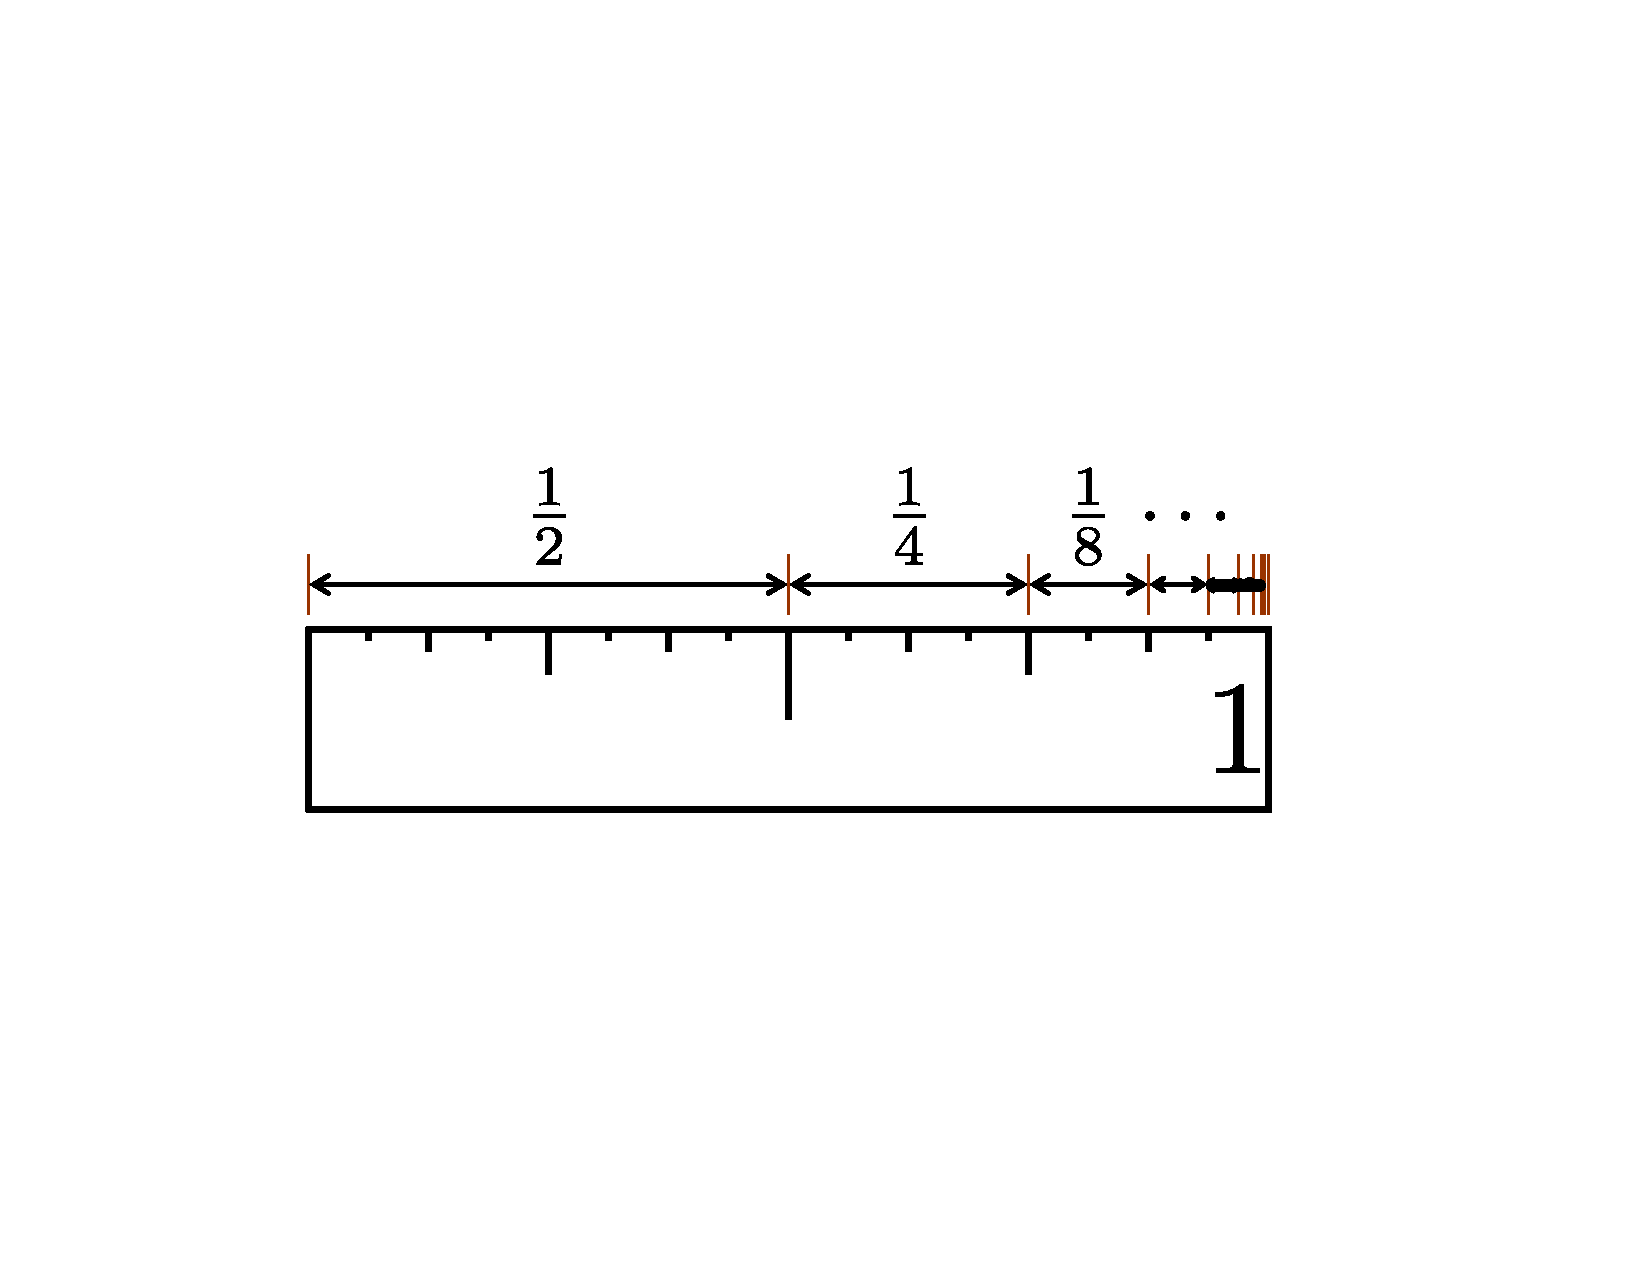
\includegraphics[width=5cm]{pic/GeometricSegment.pdf}
%\end{center}
%\end{figure}
%
%However if we look at the distance traveled after $k$ iterations, we
%get a geometric sum with ratio $\frac{1}{2}$:
%\[
%\frac{1}{2}+\frac{1}{4}
%+\frac{1}{8}+\frac{1}{16}+\cdots+\frac{1}{2^k}
%\]
%If the process continues infinitely many times, we thus get get the
%following formula for the distance traveled:
%\[
%\frac{1}{2} + \frac{1}{4} + \frac{1}{8} + \ldots + \frac{1}{2^{n}} +
%\ldots = \sum_{n=1}^{\infty} \frac{1}{2^{n}}
%\]
%We will see that this sums up to $1$ (i.e. the full distance is traveled,
%resolving the paradox).

%Notice that there is a slight shift in this formula from the one
%given in the definition of a geometric series in that we start not
%with $r^0=1$ but with $r^{1}=\frac{1}{2}$ while in the definition
%this power is zero.  This can be fixed by letting the constant a be
%$\frac{1}{2}$, This sort of index change arises often enough that we
%will first look at how we can manipulate such infinite sums.
%
%\section*{Reindexing a Series}
%We begin this discussion with a brief reminder about the $\Sigma$ notation
%for sums.
%Given $\displaystyle{\sum_{n=1}^{k} a_{n}}$ we call n the
%\textbf{index of summation}, $a_{n}$ the \textbf{$n^{th}$ term} of
%the sum, and the \textbf{upper and lower bounds of summation} are k
%and 1
%respectively.  \\
%
%Now we consider reindexing our infinite series, notice in the
%following examples we are working with geometric series, however
%this algorithm will be useful with other
%types of series that will be discussed later. \\
%
%Most of the infinite series we have seen so far have a lower bound
%of summation of one, however their are times when we are given an
%infinite series where the lower bound of summation will be a value
%other than one. We consider first a geometric series which does not
%have a lower bound of one: $$ \frac{-1}{27} + \frac{1}{81} -
%\frac{1}{243} + \ldots + (\frac{-1}{3})^{n-1} + \ldots =
%\sum_{n=4}^{\infty} (\frac{-1}{3})^{n-1} $$ This is still a
%geometric series, however our definition requires the series to have
%the form $\displaystyle{\sum_{n=1}^{\infty} ar^{n-1}}$, so
%reindexing is required. To re-index a series we follow the following
%basic algorithm:
%\begin{Algorithm}[Re-indexing a series]\ 
%\begin{itemize}
%%\item[1] Choose a new letter to be the index of summation (m)
%\item[2] Relate m to the original index of summation (n) such that when
%n=4 we have m=1.  So we have the equation m=n-3.
%\item[3] Solve for original index of summation (n) and substitute into
%the $n^{th}$ term of the sum: $$ n=m+3 \Rightarrow
%\sum_{m=1}^{\infty} (\frac{-1}{3})^{m+3-1} = \sum_{m=1}^{\infty}
%(\frac{-1}{3})^{m+2} $$ Notice if the upper bound of summation were
%finite we would have to decrease its value by 3 as well, however
%since we are summing to infinity our upper bound of summation will
%remain infinite.
%\item[4] Solve for an a such that the power on r is m-1. $$
%\sum_{m=1}^{\infty} (\frac{-1}{3})^{m+2} = \sum_{m=1}^{\infty}
%(\frac{-1}{3})^{3} \cdot (\frac{-1}{3})^{m-1}$$ since m-1+3=m+2.
%\end{itemize}
%\end{Algorithm}
%Therefore $a=(\frac{-1}{3})^3 = \frac{-1}{27}$ and $r=\frac{-1}{3}$
%so we have a geometric series of the form
%$\displaystyle{\sum_{m=1}^{\infty} ar^{m-1}}$.  Notice that in this
%example the ratio was negative, therefore a geometric series can
%have negative or positive r values. We now look at another example
%of this re-indexing algorithm before we develop an equation for the
%value of a geometric series.
%
%\begin{Example}
%Consider the series $\displaystyle{\sum_{n=9}^{\infty}
%\frac{4}{2n+3}} $, rewrite
%this series so that the lower bound of summation is n=1.
%
%\solution
%Let $m=n-8$, then $n=m+8$ so we have
%$\displaystyle{\sum_{m=1}^{\infty} \frac{4}{2(m+8)+3} =
%\sum_{n=1}^{\infty} \frac{4}{2m+19}}$
%\end{Example}
%
%Using this algorithm we can always manipulate a given geometric
%series so that it can be written in the form
%$\displaystyle{\sum_{n=1}^{\infty} ar^{n-1}}$ or equivalently
%$\displaystyle{\sum_{n=0}^{\infty} ar^n}$ next we consider how to
%calculate the value of this series.
%
%\subsection*{The Formula for the Geometric Series}
%In this section we will derive a general formula for the value of
%$\displaystyle{ \sum_{n=0}^{k} ar^{n}}$. We can apply this in the
%%limit case $k=\infty$ to get the value of an infinite series, for
%example to show that the series $\displaystyle{\sum_{n=1}^{\infty}
%\frac{1}{2^n}}$ from Zeno's paradox has value $1$.

Now consider
\[
p_{k}=a + ar + ar^{2} + \ldots + ar^k
\]
and
\[
rp_{k} = ar + ar^{2} + ar^{3} + \ldots + ar^{k+1}.
\]
Notice that these two expressions share several terms in common, in
fact
\[
p_{k}-rp_{k}= (a + ar + ar^{2} + \ldots + ar^k) - (ar +
ar^{2} + ar^{3} + \ldots + ar^{k+1}) = a -ar^{k+1}
\]
Now if we factor both sides of this equation, we get
\[
p_{k}(1-r)=a(1-r^{k+1}).
\]
As
long as $r \neq 1$ we can divide both sides by $(1-r)$ to get
%\begin{center}
%\fbox{\begin{minipage}{3in}
%\Large
\[
p_{k}=\sum_{n=0}^{k}ar^n=a\frac{1-r^{k+1}}{1-r}.
\]
%\end{minipage}}
%\end{center}

(What happens in the case where r=1?
We get $s_{k}= a + a(1) + a(1)^{2} + \ldots + a(1)^{k-1}=ka$.)
\medskip

Before we go on to get a formula for the infinite sum, we see
how the formula for $p_{k}$ might be used on its own:
%\begin{Example}[The magnitude of repeated growth]
Suppose we are given a chess board and place one grain of rice on
the first square, two grains of rice on the second square, four
grains of rice on the third square continuing on so that there are
$2^{n-1}$ grains of rice on the $n^{th}$ square.  How many grains of
rice are on the chess board? (There are $8\cdot 8=64$ squares on a chess
board.) 
%\begin{figure}
% \epsfig{file=Chess-board-walnut.jpg,scale=.8}
%\end{figure}

%\solution
Since there are 64 squares on the chess board (from $0$ to $63$), we want to compute
$p_{63}$.  Our ratio is 2 and $a$ is one, hence we are asked to find
\[
p_{63}=1+2+4+ \ldots +2^{63} =
\frac{1(1-2^{64})}{1-2} = 1.84467 \times 10^{19}
\]
%\end{Example}

A similar calculation underlies the repayment of loans or mortgages:

%\begin{Example}[Paying back a loan]
Suppose we take out a loan of $L$ dollars which is paid back
periodically (typically monthly). The periodic payment is $a$
dollars, the fixed interest rate \textit{per period} is $i$. If
$b_k$ is the loan sum outstanding after $k$ time periods, we have
that
\[
b_{k+1}=b_k\cdot (1+i)-a.
\]
Using $b_0=L$ and setting $r=1+i$, in the first step we have
\[b_{1}=Lr-a\] we then continue on to the next step where we
get
\begin{eqnarray*}
b_{2}&=&b_{1}(r)-a 
=(Lr-a)(r)-a \\
&=&Lr^{2}-(a+ar)
\end{eqnarray*}
We might be starting to notice a pattern, however it becomes obvious
in the next step
\begin{eqnarray*}
b_{3}&=&b_{2}(r)-a 
=(Lr^{2}-(a+ar))(r)-a \\
&=&Lr^{3}-(a+ar+ar^{2})
\end{eqnarray*}
At this point we can solve this recursion to
\[
b_k=L\cdot r^k-\left(a+ar+ar^2+\cdots+ar^{k-1}\right)
=L\cdot r^k-\sum_{n=0}^{k-1}ar^n
\mathop{=}\limits^{\mbox{\quad Sum formula\quad}}L\cdot r^k-a\frac{1-r^k}{1-r}.
\]
A bank now would set $b_m=0$ (where $m$ is the time after which the loan
should be paid off, e.g. $m=12\cdot 30=360$ for a 30 year mortgage)
and solve for $a$ to determine the
necessary monthly repayment, given the loan sum and interest rate.

For example, if we have a mortgage of $L=\$200,000$, an annual
interest rate of $6$\% (leading to a monthly rate of
$i=.06/12=0.005$, i.e. $r=1.005$) and a monthly repayment
sum\footnote{Slightly moralistic remark: Incidentally, initial interest amounts
to {\$}$1000$ per month at the start of the loan. An
\textit{interest only} loan thus does not save much and is a very
bad deal!} of $a=\$1,200$, we find that the outstanding sum after
$k$ months is
\[
b_k=200,000\cdot{1.005^k}-1,200\frac{1.005^k-1}{0.005}
=200,000\cdot{1.005^k}-240,000\left(1.005^k-1\right).
\]
After $10$ years ($120$ months) this leaves an outstanding amount of
{\$}$167,224.13$, after $20$ years {\$}$107,591.82$, roughly
half\footnote{In general, this means that a loan is paid off half
after roughly $\frac{2}{3}$ of its planned life time}, after $30$
years {\$}$-903.00$ (i.e. the loan is paid off after $30$ years less
one month\footnote{The total cost of the loan then will have been
{\$}$430,800$, more than double the loan amount. (Though inflation
means that the actual value will be less.)}).

If the interest rate instead was $7$\% annually ($i=.07/12=0.005833$
monthly), we get with same repayment sum a remaining loan amount of
{\$}$159,256.18$ after $30$ years, which is not even halfway paid
off. A monthly repayment sum of {\$}$1330$ would be
needed\footnote{I.e. a change of one percentage point in the
interest rate increased the monthly payment (and thus the total loan
cost) by $10$\%! No wonder people go bonkers about interest rates.}
to have the loan paid off after $30$ years.
%\end{Example}
\medskip

Since the sequence $p_0, p_{1}, p_{2}, 
\ldots, s_{k}, \ldots$ of partial sums converges to
$\displaystyle{\sum_{n=1}^{\infty} ar^{n-1}}$, we can use the
formula just derived to compute a value for the limit of a geometric series:

If $\sz{r}<1$, we have that $\lim_{k\to\infty} r^{k+1}=0$ and thus

\[
\sum_{i=0}^{\infty} ar^i
=
\lim_{k\to\infty} p_k=
\lim_{k \rightarrow \infty} \frac{a (1-r^{k+1})}{1-r} =
\frac{a(1-0)}{1-r}=\frac{a}{1-r}.
\]
This incidentally verifies the above example
\[
\sum_{i=0}^\infty \frac{1}{2^i}=2
\]

On the other hand, if $\sz{r}\ge 1$, the absolute value of the numerator
$1-r^{k+1}$ will go towards infinity, and the series diverges.


%\begin{center}
%\fbox{\begin{minipage}{\textwidth}
%\begin{Theorem}
%The geometric series $\displaystyle a + ar + ar^{2}+ \ldots +
%ar^{n-1} + \ldots =\sum_{n=1}^{\infty} ar^{n-1}$ converges to
%$\displaystyle\frac{a}{1-r}$ when $|r|<1$, and diverges otherwise.
%\end{Theorem}
%\end{minipage}}
%\end{center}
%\begin{proof}
%\textbf{Case 1:} If $|r|<1$ then $|r|^{k} <1$, and as $k$ gets
%larger this will cause $|r^{k}|$ to get smaller and yield
%$\displaystyle\lim_{k \rightarrow \infty} r^{k}=0$. Thus, by the rules for
%limits,
%
%\\
%\textbf{Case 2:} When $|r| \geq 1$ then $|r|^{k} \geq
%1$. Therefore when $k$ tends to infinity the numerator $a(1-r^{k})$
%tends to plus or minus infinity, and the denominator $1-r$ is a fixed
%value. So $\displaystyle{\lim_{k \rightarrow \infty}
%\frac{a
%(1-r^{k})}{1-r}}$ diverges.
%\end{proof}
%
%Now that we have a formula for the value of a geometric series let
%us verify the solution to the Zeno's paradox example.  We are
%looking at $\displaystyle{\sum_{n=1}^{\infty}\frac{1}{2^n}}$. First
%notice that this sum is not in the correct form,  we must factor
%$(\frac{1}{2})$ out of the $n^{th}$ term.  We get
%$\displaystyle{\sum_{n=1}^{\infty} ( \frac{1}{2})^{n} =
%\sum_{n=1}^{\infty}(\frac{1}{2})\cdot(\frac{1}{2})^{n-1}
%=\sum_{n=0}^{\infty} (\frac{1}{2}) \cdot (\frac{1}{2})^{n}}$, hence
%$a=\frac{1}{2}$ and $r=\frac{1}{2} < 1$ so this series converges to
%\[
%\frac{a}{1-r} =
%\frac{\frac{1}{2}}{1-\frac{1}{2}}=\frac{\frac{1}{2}}{\frac{1}{2}}=1.
%\]

%Next we will look at some interesting examples where we can use this
%formula.
%
%\section*{Examples}
%In this section we will look at how people may use geometric series
%in real life applications.
%
%In our first example we
%look at how much
%medication will remain in a persons body after taking medication at
%regular intervals
%\begin{Example}[Repeated Drug Dosage]
%A CSU student comes down with bacterial laryngitis, the student goes
%to the Healthcenter to see a doctor who prescribes 250mg doses of
%antibiotics that the student must take every six hours over the next
%several days.  Since the body will digest the antibiotics between
%doses and it is known that 5 percent of the drug remains in the body
%at the end of six hours, how can we calculate the quantity of the
%drug that remains in the student after the fifth dose? At the end of
%five full days on the drug?
%
%\solution
%Let us begin by looking at the quantity of the drug in the body
%after each dose.  Let $q_{n}$ represent the quantity of the drug in
%the students body after the $n^{th}$ dose.  Initially $$ q_{1}=250$$
%at the next dose we will have 5\% of that 250mg remaining and
%another 250mg is taken, so $$q_{2}=250(0.05)+250$$ At the third dose
%we have 5\% of $q_{2}$ remaining and another 250mg is taken, so
%therefore
%\begin{eqnarray*}
%q_{3}&=&0.05 \cdot q_{2} +250 =0.05(250(0.05)+250) +250\\
%&=&250(0.05)^{2} + 250(0.05) + 250.
%\end{eqnarray*}
%Now on the fourth dose
%$q_{4}$ we have $0.05 \cdot q_{3}$ remaining in the body and another
%250mg is taken.
%\begin{eqnarray*}
%q_{4}&=&0.05 \cdot q_{3} + 250
%=0.05(250(0.05)^{2} + 250(0.05) + 250) + 250\\
%&=&250(0.05)^{3} + 250(0.05)^{2} + 250(0.05) + 250.
%\end{eqnarray*}
%Notice at this point that a
%pattern has developed, we have $$q_{n}=s_{n}=\sum_{k=1}^{n}
%250(0.05)^{n-1}$$ Therefore we can use our formula
%%$s_{n}=\frac{a(1-r^{n})}{1-r}$ to calculate
%$q_{n}=\frac{250(1-0.05^{n})}{1-0.05}$.  With this information we
%can calculate $q_{5}=\frac{250(1-0.05^{5})}{1-0.05} = 263.1578125$mg
%in the students body after 5 doses.  If the student continues to
%take the antibiotic for 5 full days or 20 doses they will have
%$q_{20}=\frac{250(1-0.05^{20})}{1-0.05}=263.1578947$mg. \\
%
%Suppose the student continued to take this drug forever, how much
%medication would there be in the students body at each dose?\\
%
%This question is asking us to compute
%$\displaystyle{\sum_{n=1}^{\infty} 250(0.05)^{n-1}}$ which luckily
%for the student $0.05<1$ will converge to a finite number of
%$\frac{250}{1-0.05}=263.1578947$mg. Since $0.05^{20}=9.536743 x
%10^{-27}$ which is practically zero, we get the same value up to the
%ten-millionth place if the student took the medication forever as we
%got when the student took the medication for five days.
%
%\end{Example}
%
%\begin{Example}[Repeating Decimal]

As an example application of this formula, we look at how one can
express the repeating decimal $0.\overline{08}$ as a fraction of two integers.

%\solution
%To express $0.\overline{08}$ as a fraction 
We first notice that $08$
is the repeated value, so we want to break up $0.\overline{08}$ into
a sum of the repeated values.  Therefore we have $0.\overline{08}=
0.\underline{08}+ 0.00\underline{08}+ 0.0000\underline{08}+ \ldots$.
Once we have this written as a sum we can now write each term in the
sum as a fraction, hence we have $0.\underline{08}=\frac{8}{100}$,
$0.00\underline{08}=\frac{8}{10,000}=\frac{8}{100^{2}}$, and
$0.0000\underline{08}=\frac{8}{100^{3}}$.  Using this information we
should recognize a pattern $$0.\overline{08} = \frac{8}{100} +
\frac{8}{100^{2}} + \frac{8}{100^{3}} + \ldots = \sum_{i=1}^{\infty}
\frac{8}{100^{i}}$$ However at this point we notice that we have a
geometric series which is not written in the correct form for us to
apply our formula.  If we factor out $(\frac{8}{100})$ we get
$\displaystyle{\sum_{i=0}^{\infty}
(\frac{8}{100})(\frac{1}{100})^i}$ which is now in the correct
form. This gives $r=\frac{1}{100} <1$ so our geometric series
converges and since $a=\frac{8}{100}$ the series converges to
$$\frac{\frac{8}{100}}{1-\frac{1}{100}}=\frac{\frac{8}{100}}{\frac{99}{100}}=\frac{8}{99}=0.\overline{08}.$$
%Being able to express a repeating decimal as a fraction is useful
%when we are calculating with a large number of values where the
%precision of the answer is vital since a fraction will not have
%any round off error.  \\
%\end{Example}

For another example, consider the following paradox of Zeno\footnote{Zeno
of Elea, Greek philosopher, ca. 490 BC - ca. 430 BC}:

Achilles, the fastest runner in ancient Greece, runs 100 times as
fast as the Tortoise. But --- so the paradox claims --- if the
Tortoise is given an advance, Achilles will never be able to pass
the Tortoise:

%\begin{Example}[Achilles and the Tortoise]
Suppose that Achilles runs
$10 m/s$ and the Tortoise only $0.1 m/s$, furthermore the Tortoise is given
a head start of $100m$.
After $10$ seconds, Achilles has reached the place where the Tortoise
started. But in this time, the Tortoise has run $1m$ ahead. Achilles will
reach this distance in $0.1$ seconds. But then the Tortoise has moved
another $0.01m$. Achilles will take $0.001$ seconds to reach this, and so
on. He will never reach the Tortoise. Where is the error in this argument?

%\solution
The paradox is resolved, if we realize what time period is considered:
All events take place within
\[
10+0.1+0.001+\cdots=10\sum_{n=0}^\infty
\frac{1}{100^n}=\frac{10}{1-\frac{1}{100}}=\frac{1000}{99}=10.\overline{10}
\]
seconds. This is exactly the time {\em when Achilles reaches (and
overtakes!) the Tortoise}. The paradox arises from the implicit
(and wrong, as we have calculated!)
suggestion, that it describes the events for all time.
%\end{Example}

\section{Arithmetic Series}

While not directly related to the Geometric Series, this seems to be an
appropriate place to also look at summations over other sequences.

The summation over a constant sequence with fixed value $a$,
\[
\underbrace{a+a+\cdots +a}_{\mbox{$n$ terms}}=n\cdot a
\]
is basically just the definition of multiplication. But what happens if the
terms change by a constant sum, that is we have that $a_{i+1}-a_i=c$
constant.

Let us first observe this for the basic case of 
\[
S_n=\sum_{i=1}^n i=1+2+\cdots+n.
\]
We get a formula by writing this sum down a second time in reversed order
and add both up (thus getting {\em twice} the value $S_n$):
\[
\begin{array}{ccccccc}
&1&+2&+3&+\cdots&+(n-1)&+n\\
+&n&+(n-1)&+(n-2)&+\cdots&+2&+1\\
\end{array}
\]
We can get the value in another way by first adding down in each column.
Note that each column adds up to $n+1$, and we have $n$ columns, and this
sum thus is $n(n+1)$. This gives us the formula:
\[
\sum_{i=1}^n i=1+2+\cdots+n=\frac{n(n+1)}{2}.
\]
For example, we get that
\[
1+2+\cdots+100=\frac{100\cdot 101}{2}=\frac{10100}{2}=5050.
\]
If subsequent terms differ by a different constant, we can handle this with
a factor (and possibly a starting term. Suppose we start at 5 and differ by
3 in each step:
\[
5+8+11+14+\cdots+32
\]
we subtract $2$ from each summand, so that they all are a multiple of $3$,
and then separate the two operations:
\[
=(2+3)+(2+6)+(2+9)+\cdots(2+30)=\underbrace{2+\cdots+2}_{\mbox{$10$ terms}}
+3\left(1+2+\cdots+10\right)
\]
We know that there are 10 terms, as we have $(32-5)/3=9$ steps from the
first. Now we use the two kinds of formulas and get
\[
5+8+11+14+\cdots+32=10\cdot 2+ 3\cdot\left(\frac{10\cdot
11}{2}\right)=20+3\cdot 55=185.
\]
We note, without proof, the similar formulas:
\begin{eqnarray*}
\sum_{i=1}^n i^2&=&\frac{n(n+1)(2n+1)}{6}\\
\sum_{i=1}^n i^3&=&\frac{n^2(n+1)^2}{4}\\
\end{eqnarray*}

%\subsection{Other Sums}
%
%there is a constant factor $a$, such that
%every term is the $a$-times multiple of the previous term. That is
%
%The partial sums over this sequence are thus
%\[
%\sum_{j=0}^i a^i r = r\cdot\sum_{j=0}^i a^i
%\]
%Multiplying this expression by $1-a$ gives us
%\begin{eqnarray*}
%(1-a)(r\sum_{j=0}^i a^j)&=&r\left(\sum_{j=0}^i a^j-a\sum_{j=0}^i a^j\right)\\
%&=&r\left(\sum_{j=0}^i a^j-\sum_{j=1}^{i+1} a^j\right)=r\left(a^0-a^{i+1}\right)
%=r\left(1-a^{i+1}\right)
%\end{eqnarray*}
%and (dividing again by $1-a$)
%\[
%\sum_{j=0}^i ra^i=r\frac{1-a^{i+1}}{1-a}
%\]
%This formula is called the summation formula for the geometric series and has many
%practical applications.


\chapter{Differentiation}
\label{chdiff}

We are now almost ready to start looking at the concepts of Calculus. The
underlying idea is that we should be able to describe the values of a
function, or its long term behavior, based on how it changes locally.

\section{Function limits and Continuity}

Before defining the derivative of a function on the real numbers, 
there are some, somewhat
technical concepts, we need to touch upon:

First, we want to extend the concept of the limit of a sequence (at
$\infty$) to the limit of a function at a point.
\begin{defn}
Let $f\colon\R\to\R$ be a function and $a\in\R$. If, for every sequence
$\{a_n\}$ with $\lim_{n\to\infty} a_n=a$, the sequence of function values
$\{f(a_n\}$ also converges to $L=\lim_{n\to\infty} f(a_n)$, and the limit
$L$ does not depend on the choice of the sequence, we call this the limit
of $f$ at $a$, written
\[
\lim_{x\to a} f(x)=L
\]
\end{defn}

(Calculating such a limit can potentially be hard, as one has to consider an
infinitude of possible sequences.)

For many functions occurring in the real world, this limit is equal to the
function value $f(a)$, since nature does not jump, but this is not
guaranteed for every function.

\begin{figure}[t]
\begin{center}
\includegraphics[width=8cm]{pic/DiscontFct.png}
\end{center}
\caption{Some discontinuous functions}
\label{figdiscont}
\end{figure}

Our definition of functions however allows for {\em arbitrary} functions, such as the
following ones (Figure~\ref{figdiscont}):
\begin{eqnarray*}
f\colon\R\to\R&,& x\mapsto \lfloor x\rfloor\qquad\mbox{Round down to integer}\\
g\colon\R\to\R&,& x\mapsto 
\left\{\begin{array}{ll}
\sin(1/x)&x\not=0\\
1&x=0\\
\end{array}
\right.\\
h\colon\R\to\R&,& x\mapsto 
\left\{\begin{array}{ll}
3&x\in\Q\\
-3&x\not\in\Q\\
\end{array}
\right.
\end{eqnarray*}
If we investigate the function $f$ around $1/2$, there is no way to see that it jumps at
0 and at 1. Similarly, why is the value of $g$ at $0$ one (and not zero or $-1$, or
something in between). And we can't even look fine enough to decide from the graph that
$h$ is a function.

Instead, we want that the graph of the function is smooth, that is that we get close to
a point $x$, we can predict the function value $f(x)$. Getting closer will ultimately
give a better approximation.

Formally, we define a function $f\colon\R\to\R$ to be~\defini{continuous} at a point $x_0$
(otherwise: \defini{discontinuous}) if
\begin{quote}
The limit $\displaystyle\lim_{x\to x_0} f(x)$ exists and is equal to the
function value $f(x_0)$.
\end{quote}

If the function is continuous at every point $x_0$, we simply call it continuous (without
``at'').

We see for example that the ``rounding down'' 
function $f(x)=\lfloor x\rfloor$  is not continuous at $1$,
since the sequence $a_i=1-1/i$ has $\lim_{i\to\infty} a_i=1$, but
$f(a_i)=f(1-1/i)=\lfloor 1-1/i\rfloor=0$, and thus $\lim_{i\to\infty}
f(a_i)=0i\not=1=f(1)$.
\medskip

Informally, a function is continuous, if small changes in the argument imply small
changes in the value -- that is we can approximate the function value at $x_0$ by the 
function values at numbers close to $x_0$. For the graph of the function
this means that it may not have any jumps, nor start wild oscillations, but
should be followed easily with a pencil. Most functions you will encounter
(that do not jump) are likely to be continuous.

To show formally that a function is continuous, using the definition, can be
hard.  We therefore do not investigate
this further in this class\mynote{There is a criterion that is used in the Calculus class for mathematicians
that formalizes the ``close approximation'' idea, but we do not need it here}. Instead
we study what continuity is good for.

\subsection{Some continuous functions}

Many functions you know from school are continuous. And due to the laws of
limits it is not just these functions, but also functions composed by
arithmetic operations (as long as a denominator does not become zero), and
also compositions of such functions:

\begin{itemize}
\item Nonnegative powers of $x$: $x^a$ for $a\in\R$. This includes the constant function
$x^0$.
\item Thus also polynomials and (as long as the denominator is nonzero) rational
functions.
\item Trigonometric functions $\sin(x)$, $\cos(x)$, and $\tan(x)=\sin(x)/\cos(x)$ (when
the denominator is nonzero).
\item Inverse trigonometric functions (Note that $\arcsin$ and $\arccos$ are only defined
on the domain $\{-1\ldots 1\}$.
\item The exponential function $\exp(x)=e^x$ and (for positive $x$) its
inverse the natural logarithm $\log(x)=\ln(x)$. (All logarithms in this
course without a specific basis are natural logarithms.)
\end{itemize}

The definition of some of these functions (such as $\sin(x)$ as measurement
on a triangle in a circle) given in
school is not amenable to easy computation, we will see later
\pointer{sectaylors} how this can be done.

\section{Why Care About Continuity}
\label{secwhycont}

The first use of continuity is that it makes approximation meaningful. We can work, for
example, with numerical approximations of $x$ values, and trust that the function value
$f(x)$ will not differ too much from $f(x_0)$ if $x$ is an approximation of $x_0$.

A consequence of this is that we can ``control'' the function values. If we want to find
$x$ to achieve a particular function value $f(x)$, we can do so by iterative
approximation. On the other hand, the situation that small changes in the input could
produce (arbitrary) large changes in the output is close to the definition of chaos.
\smallskip

A consequence of this property is the following statement:
\begin{figure}
\begin{center}
\includegraphics[width=6cm]{pic/IntermedThm.pdf}
\end{center}
\caption{The intermediate Value Theorem}
\label{figivt}
\end{figure}
\begin{thm}[Intermediate Value Theorem]
Let $f\colon\R\to\R$ be a continuous function and $x_1<x_2\in\R$ with $f(x_1)=a$ and
$f(x_2)=b$. Let $c$ be a number between $a$ and $b$. Then there exists $x_1\le x\le x_2$
such that $f(x)=c$ (Figure~\ref{figivt}).
\end{thm}

We can use this theorem to find $x$ for a particular $f(x)$-value. Most frequently this
is done to find $x$, such that $f(x)=0$. The method is called \defini{halving
intervals} or \defini{bisection} method.
\begin{enumerate}
\item
Start with $s,t\in\R$ such that $f(s)<0$ and $f(t)>0$. (Or vice versa: $f(s)>0$ and
$f(t)<0$.)
\item Let $m=\frac{s+t}{2}$ be the midpoint of the interval. If $f(m)=0$ and
stop. Otherwise:
\item If $f(s)$ and $f(m)$ have the same sign (positive or negative) replace $s$ by $m$.
Otherwise replace $t$ by $m$ (since $f(m)$ and $f(t)$ have the same sign).
\item If $\sz{t-s}$ is not small enough (to the approximation quality we want), go to
step 2.
\end{enumerate}
In each step of the algorithm, the length of the interval from $s$ to $t$ halves, and
the desired $x$ value must lie in the interval. We can repeat until $s$ and $t$
approximate this $x$ sufficiently well.

For example, consider the function $f(x)=\sin(x)$. We want to approximate the number
$\pi$, knowing\mynote{We measure the angle of a full circle as $2\pi$}
that $f(\pi)=0$. We start with $s=2$ and $t=4$, since we know that
$2<\pi<4$. We now iterate, setting $m=(2+4)/2=3$ and calculate $f(3)$, which is
positive. Thus we replace $s$ by $3$ and iterate. The following table shows the
further iterations (with underlined numbers indicating the end point that was replaced
by $m$ in each step).
After 20 iterations, the length of the interval has become $2/2^{20}\sim 10^{-6}$. This
agrees with the fact that we gain a further correct digit every
$\log_2(10)\sim 3.3219$ steps and thus should expect $20/3.3219=6$ correct digits in the result,
approximating $\pi$ as $3.141593$ (versus the correct\mynote{Count the digits in each
word in the sentence {\em
How I want a drink, alcoholic of course, after the heavy chapters involving quantum
mechanics}.} $3.1415926\ldots$).
\begin{center}
\begin{tabular}{@{}rl@{\,\,\,\,}l@{\,\,\,\,}l@{\,\,\,\,}l@{\,\,\,\,}l@{\,\,\,\,}l@{\,\,\,\,}l@{}}
\#&$s$&$t$&$\sz{t-s}$&$f(s)$&$f(t)$&$m=\frac{s+t}{2}$&$f(m)$\\
0&2&4&2&0.909297&-0.756802&3&0.141120\\
1&\underline{3}&4&1&0.141120&-0.756802&3.5&-0.350783\\
2&3&\underline{3.5}&0.5&0.141120&-0.350783&3.25&-0.108195\\
3&3&\underline{3.25}&0.25&0.141120&-0.108195&3.125&0.016592\\
4&\underline{3.125}&3.25&0.125&0.016592&-0.108195&3.1875&-0.045891\\
5&3.125&\underline{3.1875}&0.0625&0.016592&-0.045891&3.156250&-0.014657\\
6&3.125&\underline{3.15625}&0.03125&0.016592&-0.014657&3.140625&0.000968\\
7&\underline{3.140625}&3.156250&0.015625&0.000968&-0.014657&3.148438&-0.006845\\
8&3.140625&\underline{3.148438}&0.007813&0.000968&-0.006845&3.144531&-0.002939\\
9&3.140625&\underline{3.144531}&0.003906&0.000968&-0.002939&3.142578&-0.000985\\
10&3.140625&\underline{3.142578}&0.001953&0.000968&-0.000985&3.141602&-0.000009\\
11&3.140625&\underline{3.141602}&0.000977&0.000968&-0.000009&3.141113&0.000479\\
12&\underline{3.141113}&3.141602&0.000488&0.000479&-0.000009&3.141357&0.000235\\
13&\underline{3.141357}&3.141602&0.000244&0.000235&-0.000009&3.141479&0.000113\\
14&\underline{3.141479}&3.141602&0.000122&0.000113&-0.000009&3.141541&0.000052\\
15&\underline{3.141541}&3.141602&0.000061&0.000052&-0.000009&3.141571&0.000022\\
16&\underline{3.141571}&3.141602&0.000031&0.000022&-0.000009&3.141586&0.000006\\
17&\underline{3.141586}&3.141602&0.000015&0.000006&-0.000009&3.141594&-0.000001\\
18&3.141586&\underline{3.141594}&0.000008&0.000006&-0.000001&3.141590&0.000003\\
19&\underline{3.141590}&3.141594&0.000004&0.000003&-0.000001&3.141592&0.000001\\
20&\underline{3.141592}&3.141594&0.000002&0.000001&-0.000001&3.141593&-0.000000\\
\end{tabular}
\end{center}
Such a process of halving intervals can be implemented easily. It however
takes a while to get a good approximation, which is why we will see a better
method in a later chapter~\pointer{secnewton}.

\section{Partial Sums and Derived Sequences}

Before defining derivatives properly, let us look at an example of change
that happens at discrete intervals, and how function values and change are
related.


Imagine
the ledger of a business that lists every day the sum of income minus expenses
(let's call it the \defini{flow}), and the total money held by the business:

\begin{center}
\begin{tabular}{rrr}
Day&Income-Expenses&Money held\\
\hline
0& - &0\\
1&893&893\\
2&70&963\\
3&992&1955\\
4&682&2637\\
5&115&2752\\
6&215&2967\\
7&-497&2470\\
8&-246&2224\\
9&252&2476\\
10&-301&2175\\
\end{tabular}
\end{center}

Going through the columns, we get two sequences, both indexed by the first
column.  The first sequence, which we shall call $a_i$ is the daily flow.
The second sequence, let's call it $b_i$, is the money held by the business.
Is there a relation between the two columns?

Of course. Assuming we started with $0$ money held, the money held on the end of day
$i$ is the sum of the flow of days $1$ to $i$. We write this as
$$b_i=a_1+a_2+a_3+\cdots+ a_{i-1}+a_i=\sum_{j=1}^i a_j$$
and have that the $b_i$ are the *partial sums* over the sequence $a_i$.

Can we do the same thing backwards? Surely -- solving for $a_i$ finds that
$$a_i=\sum_{j=1}^ia_i-\sum_{j=1}^{i-1}a_i=b_i-b_{i-1}.$$

The two sequences are thus "related" in that each sequence completely
determines the other one and vice versa. We shall call the sequence $\{a_i\}$
the \defini{derivative sequence} of the sequence $\{b_i\}$ and the sequence
$\{b_i\}$ 
an \defini{antiderivative} or an
\defini{indefinite integral} of $\{a_i\}$.

Calculus is about studying such a correspondence between functions defined on
(e.g.) the real numbers, while sequences are functions defined on the
positive integers.

Before going there, let us look at a few ways how this correspondence plays
out and helps us with determining information.
First, imagine we would have started not at 0 but with some money in the
bank, say 1000 currency units. Then the ledger would have looked almost the
same, but for the last column being increased by 1000:

\begin{center}
\begin{tabular}{rrr}
Day&Income-Expenses&Money held\\
\hline
0& - &1000\\
1&893&1893\\
2&70&1963\\
3&992&2955\\
4&682&3637\\
5&115&3752\\
6&215&3967\\
7&-497&3470\\
8&-246&3224\\
9&252&3476\\
10&-301&3175\\
\end{tabular}
\end{center}

Denote the sequence given by the third column in this ledger by $c_i$. We
note that $c_i$ is built from the *same changes* as $b_i$ is. Thus $a_i$ is
also the derivative of $c_i$ and $c_i$ is an integral of $a_i$. (That is why
we said ``an integral'' and not ``the integral''.) It is not hard to see that
there are many more antiderivatives (namely different starting values in the
bank), but that any two antiderivatives simply differ by a constant (namely
the difference of their starting account values).

If we care about the flow over a number of days, say from day 4 to day 7
(inclusively), we need to add up the flows of these three days:
$$a_4+a_5+a_6+a_7=\sum_{j=4}^7 a_j.$$
Using the sum notation, we see that this multi-day flow difference also can
be expressed as a difference of values of an antiderivative over multiple
days, we have that
$$\sum_{j=4}^7 a_j=(\sum_{j=1}^7 a_j)-(\sum_{j=1}^3 a_j)=b_7-b_3=c_7-c_3.$$
Here $7$ is the time when the counting ends (the evening of day 7) and $3$
the time when it starts (the evening of day $3$ as giving the same amount as
on the morning of day $4$ which is not listed separately in the ledger.)

This difference formula will hold for whatever antiderivative we are
choosing. This holds, because the starting account value has no impact on
the flow over the four days we are measuring. Thus antiderivatives (more
specifically the {\em difference} of the values of antiderivatives between a
start and an end point, which will be called a \defini{definite integral}.)
We will encounter this easy idea later again under the name of
``Fundamental Theorem of Calculus''.
\medskip

We have seen that an antiderivative helps with summing up changes over a
period. But what can derivatives be used for? To illustrate this, look at
a different sequence $\{b_i\}$ (starting with $b_0$) whose changes are smaller, but which we tabulate
over a longer range:
\begin{eqnarray*}
&&
 0, 8, 15, 21, 24, 26, 28, 26, 25, 23, 21, 19, 18, 16, 15, 14, 13, 14, 15,
  16, 18, 20, 22, 25,\\
 &&\qquad 28, 31, 34, 37, 40, 43, 46, 48, 50, 51, 52, 53, 52, 51,
  49, 48, 45, 42, 40, 36, 33,\\
  &&\qquad 31, 28, 27, 26, 27, 30 
\end{eqnarray*}
We get a sequence of changes $\{a_i\}$ (starting with $a_1$) as
$a_i=b_i-b_{i-1}$:
\begin{eqnarray*}
&&
7, 6, 3, 2, 2, -2, -1, -2, -2, -2, -1, -2, -1, -1, -1, 1, 1, 1, 2
\end{eqnarray*}
The values of both sequences are depicted (with points connected) in
Figure~\ref{figpythder}.

\begin{figure}
\begin{center}
\includegraphics[width=8cm]{pic/pythder.png}
\end{center}
\caption{A sequence and its derivative}
\label{figpythder}
\end{figure}

An obvious question one can ask for such a sequence $b_i$ is for what the
maximum and minimum (largest and smallest) values over the investigated
period are.
(In the previous example these would have been the lowest and the highest
worth of the business.) We mark the areas where the function is (locally,
that is in relation to its neighbors) maximal or minimal in
Figure~\ref{figpythder2}.

\begin{figure}
\begin{center}
\includegraphics[width=8cm]{pic/pythder2.png}
\end{center}
\caption{Maxima and Minima}
\label{figpythder2}
\end{figure}

We note that at these index values (for which the function $bn$ is maximal,
respectively minimal), which are aligned along the $x$-axis, the derivative
is zero. (An eagle-eyed reader might notice that we are slightly cheating
here: Since we sum up the values of the derivative, the maximum happens at
the $x$-value plus 1, and our derivatives are only close to zero. This will
be resolved later when we will decrease the step-width more and more.)

Furthermore, at an index $i$, where $b_i$ has minimum value, the derivative
$a_i$ changes from being negative to being positive. And at the index $i$
where $b_i$ has maximum value, the derivative changes sign from positive to
negative.  The reason for this is easily understood. To be a maximum value
(say),at index $i$m the values must have grown in step $i$ (that is the
derivative is positive at $i$), as otherwise the value cannot be larger than
other different ones. But if the derivative did not become negative at
$i+1$, the function would have been growing even further.

Thus, if we look at all places where the derivative changes from positive to
negative we see that these are exactly the *local maxima*, that is the
places where the function is larger than in the neighborhood (with the same
argument about growing before but not after).

A similar kind of argument can be made for local minima.

Finding indices where the derivative is (close to) zero is easy. The
derivative thus allows us to find maxima or minima (which are harder to
find).
\smallskip

This is a further indication that the concept of a derivative is a useful
concept, and we will spend most of the remainder of the class studying
derivatives and antiderivatives and their consequences.

\section{Aliasing}

The concept of summing up changes is rather basic, and the reader might
wonder what else there could be to Calculus. One fundamental issue is that
the prior example had a natural step-width (the day), while this is not true
for many other situations. Indeed, results might be fundamentally wrong if
we impose an artificial step-width. This phenomenon goes under the name of
\defini{aliasing} and also can occur when digitizing pictures or sound
signals. In this section (which is not required later on) we illustrate what
can happen.
\smallskip

Imagine we  have temperatures oscillating as on a typical winter day in
Colorado, with a cold mornings but temperate early afternoons. The red curve
in Figure~\ref{figalias}, left (with the $x$-axis indicating days) shows
how temperature changes over time. Now an alien (who has no concept of an
Earth day) samples the temperature, namely in intervals if $0.8$ days. The
blue dots indicate the measurements. Based on these measured values, one
clearly would expect the temperature to fluctuate periodically in a cycle of
$4$ days, as indicated by the blue curve in Figure~\ref{figalias}, right.
\begin{figure}
\begin{center}
\includegraphics[width=5cm]{pic/Aliasing1.pdf}
\quad
\includegraphics[width=5cm]{pic/Aliasing2.pdf}
\end{center}
\caption{Bad sampling leads to aliasing}
\label{figalias}
\end{figure}
Different sample periods will lead to differently bad results (a sample
period of exactly one day would indicate that 

The \defini{Nyquist}-\defini{Shannon} sampling theorem in fact shows, that
one needs to sample a periodic signal at at least twice the maximal
frequency (that is twice per period) to be able to detect these frequencies.


The same effect can be seen in so-called \defini{Moir\'e} patterns when
overlaying fabric meshes or when naively reducing the size of a digital
image, as in Figure~\ref{figscreenpic}: When reducing the image by simply
sampling pixels at regular intervals, not only does an underlying regular
grid (from taking a picture off a monitor) become overwhelming, even the
direction of the grid changes! A more sophisticated algorithm instead will
try to keep colors in local areas the same and is able to produce a much
better result (the right image has the same reduced size parameters as the
middle one).
\begin{figure}
\begin{center}
\includegraphics[width=35mm]{pic/screenphoto.png}
\quad
\includegraphics[width=35mm]{pic/screenphoto2.png}
\quad
\includegraphics[width=35mm]{pic/screenphoto3.png}
\end{center}
\caption{Image reduced by bad and by good algorithm}
\label{figscreenpic}
\end{figure}

\section{The Derivative of a Function}

We have seen that it can be useful to study how the values of a function
change. Let us look at what this means for a function defined on the real
numbers: We could, at a point $x_0$ look how the function changes between
$x_0$ and $x_0+1$ (namely by $f(x_0+1)-f(x_0)$). But there is really no
reason to take a step of $1$. We could similarly look at the change when
taking a step by $2$ or by $\frac{1}{2}$. And of course one would expect the
change to be larger if the step-width becomes larger.

\subsection{Secant Slope}

\begin{figure}
\begin{center}
\includegraphics[width=8cm]{pic/SecantSlope.pdf}
\end{center}
\caption{A secant}
\label{figonesecant}
\end{figure}

\begin{figure}
\begin{center}
\includegraphics[width=8cm]{pic/SecantSlopes.pdf}
\end{center}
\caption{Multiple secants and the tangent}
\label{figsecantslopes}
\end{figure}

We can deal with this variability by not considering the absolute change
$f(x_0+1)-f(x_0)$ by one unit, but by
considering a variable step width (which we denote by $h$ or by
$\Delta x$, $\Delta$ being used here to indicate a difference), and to
consider the change relative to the step width. That is, we consider the
fraction
\begin{equation}
\frac{f(x_0+h)-f(x_0)}{(x_0+h)-x_0}=\frac{f(x_0+h)-f(x_0)}{h}
\label{diffquot}
\end{equation}
This fraction is the slope of the line between the points $(x_0,f(x_0))$ and
$(x_0+h,f(x_0+h))$, Figure~\ref{figonesecant}. Such a line is called a \defini{secant}, as it intersects the graph
twice. The ratio in equation~(\ref{diffquot}) gives the slope of this secant, and
is called the \defini{difference quotient}.
Since the numerator is the change of
function values, sometimes this quotient is also written as $\displaystyle
\frac{\Delta f(x)}{\Delta x}= \frac{\Delta y}{\Delta x}$.

But we can choose different values of $h$ (Figure~\ref{figsecantslopes}),
and (unless the function is a line) this will yield different secants with
different slopes, depending on the value of $h$.

To remove this ambiguity we now make $h$ small. That is, we consider 
the difference quotient as a function of $h$ and study the limit
\[
\lim_{h\to 0}\frac{f(x_0+h_n)-f(x_0)}{h_n}
\]
This limit (if it exists) is the slope of the tangent line to the graph of
$f$ at $x_0$.
\smallskip

This approach immediately raises two questions:

\paragraph{Will this limit always exist?} No. It is possible that the limit
does not exist, for example if the function is not continuous at $x_0$. Also
the limit might not exist.
For example, if the graph
has a ``corner'' at $x_0$ (as the graph for $\sz{x}$ has at $x_0=0$), the
limit for a sequence of positive $h_n$ will differ from the limit of a
sequence of negative $h_n$. The formal definition thus needs to require this
limit to exist:

\begin{defn}
Let $f\colon\R\to\R$ be a function that is continuous at $x_0$. If the limit
\[
L=\lim_{h\to 0}\frac{f(x_0+h_n)-f(x_0)}{h_n}
\]
exists, then
$f$ is called \defini{differentiable} at $x_0$. The value $L$ (which is the
slope of the tangent to the graph of $f$ at $x_0$) is called the
\defini{derivative of $f$ at $x_0$} and denoted by $f'(x_0)$.
\end{defn}
Note that in particular that a function that is not continuous at $x_0\in\R$ 
is not differentiable at $x_0$. But there are continuous functions that are
not differentiable. Figure~\ref{fiUndifferentiable} shows some typical situations:
\begin{itemize}
\item The function tends to infinity (so might not even be continuous).
\item The slope becomes vertical at a point.
\item The graph of the function has a ``kink'', so there will not be a
unique tangent.
\end{itemize}
\begin{figure}[t]
\begin{center}
\includegraphics[width=5cm]{pic/Undifferentiable.pdf}
\end{center}
\caption{Not differentiable}
\label{fiUndifferentiable}
\end{figure}

\paragraph{How can we test for being differentiable,
and calculate the value of the derivative?}
Testing differentiability can be technical and is not a focus in this
course. We will see how this works in a few easy examples, but then
introduce easier rules for finding derivatives.

\section{Basic Derivatives, Polynomials}
\label{secderpol}

Let us consider a few easy cases. First, consider a constant function
$f(x)=c$. In this case $f(x_0)=c=f(x)$ for every $x$ and thus
\[
\frac{f(x_0+h_n)-f(x_0)}{h_n} =\frac{c-c}{h_n}=0
\]
and thus the limit exists, and is always equal
\[
\lim_{n\to\infty} \frac{f(x_0+h_n)-f(x_0)}{h_n}=0
\]
Therefore: A constant function is differentiable at every $x_0$, and has
derivative $f'(x_0)=0$.

Next consider the function $f(x)=x$. Then
\[
\frac{f(x_0+h_n)-f(x_0)}{h_n} =\frac{(x_0+h_n)-x_0}{h_n}=\frac{h_n}{h_n}=1.
\]
Again, the limit exists, and is always equal and we have that
$f'(x_0)=1$.

For the next cases, we will need the limit laws from
Lemma~\ref{limitlaws}: Consider the function $f(x)=x^a$ for an integer
$a>1$. Then (by the binomial theorem~\mynote{recall Pascal's triangle}) we
have that 
\[
f(x_0+h_n)=(x_0+h_n)^a=\sum_{i=0}^a {a\choose i} x_0^{a-i} h_n^i
=x_0^a+\sum_{i=1}^{a} {a\choose i} x_0^{a-i} h_n^i
\]
and thus
\begin{eqnarray*}
\frac{f(x_0+h_n)-f(x_0)}{h_n}&=&\frac{(x_0+h_n)^a-x_0^a}{h_n}
=\frac{x_0^a+\sum_{i=1}^{a} {a\choose i} x_0^{a-i} h_n^i-x_0^a}{h_n}\\
&=&\frac{\sum_{i=1}^{a} {a\choose i} x_0^{a-i} h_n^{i}}{h_n}
=\sum_{i=1}^{a} {a\choose i} \frac{x_0^{a-i} h_n^{i}}{h_n}
=\sum_{i=1}^{a} {a\choose i} x_0^{a-i} h_n^{i-1}\\
&=&a x_0^{a-1}+\sum_{i=2}^a{a\choose i} x_0^{a-i} h_n^{i-1}.
\end{eqnarray*}
But every summand in the sum on the right hand side has a factor $h_n$ and,
since $\lim_{n\to\infty h_n}=0$ we have 
$\lim_{n\to\infty}\sum_{i=2}^a{a\choose i} x_0^{a-i} h_n^{i-1}=0$ and thus
\[
\lim_{n\to\infty}\frac{(x_0+h_n)^a-x_0^a}{h_n}=a x_0^{a-1}.
\]
Once more, the limit exists and is independent of the choice of sequence
$h_n$. Thus the function $f(x)=x^a$ is differentiable at every $x_0$ and has
the derivative $f'(x_0)=a x^{a-1}$. This result subsumes (for $a=0$ and
$a=1$ the previous two, and one can show that it even holds if $a$ is an
arbitrary real number.
\smallskip

A similar application of the limit laws gives us that, if $f$ and $g$ are
differentiable at $x_0$, so is  $(f+g)(x)$ with derivative
$f'(x_0)+g'(x_0)$, as is $(cf)(x)$ (for a constant $c\in\R$) with derivative
$cf'(x_0)$.
\smallskip

Combining all of this, we have that a polynomial $f(x)=\sum_{i=0}^n a_ix^i$
is differentiable at every $x_0$ and has the derivative\mynote{and this is
all you need to remember from this section!}
\[
f'(x_0)=\sum_{i=1}^n a_i\cdot i\cdot x_0^{i-1}
\]

\section{The Derivative as a Function}

We have so far, for a given function $f$ defined a derivative at a point
$x_0$, as the slope of the tangent line to the graph of the function at
point $(x_0,f(x_0)$ and denoted it as $f'(x_0)$. Assuming the function $f$
is differentiable at every
$x_0\in\R$, we can calculate these derivative values $f'(x_0)$ for every
$x_0$ and consider $f'$ as a function itself (that assigns to $x_0$ the
value $f'(x_0)$). This function is called the derivative (function) of $f$.
Besides the name $f'$, it also is denoted by 
$\displaystyle\frac{\mbox{d}f}{\mbox{d}x}$ or
$\displaystyle\frac{\mbox{d}}{\mbox{d}x} f$, where the
$\frac{\mbox{d}}{\mbox{d}x}$ is to be considered as a particular symbol
(alluding to the difference quotient), not
as an actual fraction. In Physics, also the notation $\dot f$ is sometimes
used.

This derivative function assigns to every point $x$ the slope of the tangent
to the graph of $f$ at the point $(x,f(x))$.
We already know how to determine a formula for this derivative function for
polynomials:
\begin{bsp}
Let $f(x)=x^{5}+x^{4}-20x^{3}-20x^{2}+64x+64$.
Figure~\ref{figmultitangent} shows tangents (green) to the graph (red)of $f$
at some points. If we determine the slope of these tangents at all points
$(x,f(x))$, we get the graph (blue) of the derivative $f'(x)$.

By the result of the previous section, we actually can calculate a formula
for this derivative as $f'(x)=5x^{4}+4x^{3}-60x^{2}-40x+64$. Using
this formula, we can calculate exact values of $f'(x)$ for arbitrary points $x$, as in the following table:
\[
\begin{array}{r|rrrrrrrrr}
x&-4&-3&-2&-1&0&1&2&3&4\\
\hline
f'(x)&288&-59&-48&45&64&-27&-144&-83&480
\end{array}
\]
Note that these values agree with the slopes of the tangents.
\end{bsp}
\begin{figure}[t]
\begin{center}
\includegraphics[width=8cm]{pic/MultiTangent.pdf}
\end{center}
\caption{Multiple tangents and the derivative}
\label{figmultitangent}
\end{figure}

\begin{note}
The notation $\displaystyle\frac{\mbox{d}f}{\mbox{d}x}$ serves another
purpose, namely indicating with respect to {\em which} variable we take the
derivative. If we look at multiple functions (or functions with a
parameter), a function expression might contain other symbols, though only
one will be considered the variable with respect to which we take the
derivative. In the case of $\displaystyle\frac{\mbox{d}f}{\mbox{d}x}$ this
variable is $x$,. though one also might write
$\displaystyle\frac{\mbox{d}f}{\mbox{d}a}$ to indicate that the relevant
variable is called $a$.

Ultimately, of course such functions with be considered as being of multiple
variables, and the derivative with respect to one variable means we are
considering only a ``slice'' of the function. More about this will come in
multivariable calculus.

Here we just should note that e.g.
$\displaystyle\frac{\mbox{d}f}{\mbox{d}a}=x^2$ for $f(x)=a\cdot x^2$,
(considering $a$ as the variable and $x$ as constant), while
$\displaystyle\frac{\mbox{d}f}{\mbox{d}x}=a$ and
$\displaystyle\frac{\mbox{d}f}{\mbox{d}b}=0$.
\end{note}

\section{Derivatives of Elementary Functions}
\label{derelem}

A function is called \defini{elementary}\mynote{my dear Watson}, if it
cannot be composed from other functions. These are typically functions
that are useful in particular applications and that have their own key on the calculator, such as $\exp(x)$ or $\sin(x)$.

By careful inspection of the graphs of some of these functions it is possible
to identify expressions for their derivatives. (The ultimate justification
for some of these formulas will for us come through Taylor
series~\ref{sectaylors}.)

We note these derivative formulas in the following table:

\[
\begin{array}{c|c}
\mbox{Function $f(x)$}&\mbox{Derivative $f'(x)$}\\
\hline
\sin(x)&\cos(x)\\
\cos(x)&-\sin(x)\\
\exp(x)=e^x&\exp(x)\\
\log(x)&1/x\\
\arcsin(x)&\frac{1}{\sqrt{1-x^2}}\\
\arccos(x)&\frac{-1}{\sqrt{1-x^2}}\\
\arctan(x)&\frac{-1}{1+x^2}\\
\mbox{bla}(x)&\frac{e^x-1}{x}\\
\end{array}
\]
This table also gives an indication what is special about the basis $e$ in
the exponential function $\exp(x)=e^x$, as for this basis the function equals
its own derivative.

\begin{note}
The reader will note a function $\mbox{bla}(x)$, that she did not
encounter before. It is a made-up function that is introduced solely to
provide example problems for homework and exams that cannot be solved with standard
computational tools.
\end{note}

\section{Differentiation Rules}

When we studied functions, we looked at how we can build new functions from
simpler ones. These constructions also allow us to write down formulas for the
derivatives, as we will study in this section. We will aim to give a
justification for each of these formulas, though will not always give a
formal proof.

Let us start with some basic cases. (Some of these will end up later just
being special cases of a more general rule, so you won't have to memorize
all of this, but it is to help justifying the more general cases.)

We start with the basic transformations to a function's graph, as in
section~\ref{secfunari}. Let us look at the graph of a function under
transformations, and see how this affects the slope of a secant. (Since the
derivative is the slope of a tangent as limit of the secant slope, it will
be transformed in the same way.)

In the examples in Figure~\ref{figderbasic}, we always transform an original function $f$
(red) and its secant (orange) (from $x_0=0$ to $x_0+h=8$)
to a new function $p$ (blue, with
corresponding green secant). Recall that the slope of the secant is given as
\[
\frac{\Delta f}{\Delta x}=\frac{f(x_0+h)-f(x_0)}{x_0+h-x_0}
=\frac{f(x_0+h)-f(x_0)}{h},
\]
and that we thus only need to see how $\Delta f$ and/or $\Delta x$
transform. Note that vertical shift can be considered as a special case of
addition, and that the rules for addition and for vertical scaling 
agree with what we've seen before in Section~\ref{secderpol} for
polynomials.

\begin{figure}
\begin{tabular}{cccc}
\begin{minipage}[b]{4cm}
\includegraphics[width=4cm]{pic/picder1.png}\end{minipage}&
\begin{minipage}[b]{3cm}
\textbf{Vertical Shift:}\\
$p(x)=f(x)+3$.
Then $\Delta p=\Delta f$ and $\Delta x$ stays the same:
\[
\frac{\Delta p}{\Delta x}=\frac{\Delta f}{\Delta x}
\]
\vfill\ 
\end{minipage}&&\begin{minipage}[b]{3cm}
$p'(x)=f'(x)$.
\vspace{2cm}
\vfill\ 
\end{minipage}\\
\begin{minipage}[b]{4cm}
\includegraphics[width=4cm]{pic/picder2.png}\end{minipage}&
\begin{minipage}[b]{3cm}
\textbf{Vertical Scaling:}\\
$p(x)=2\cdot f(x)$.
Then $\Delta p=\Delta f$ and $\Delta x$ stays the same.
\[
\frac{\Delta p}{\Delta x}=2\frac{\Delta f}{\Delta x}
\]
\vfill\ 
\end{minipage}&&\begin{minipage}[b]{3cm}
$p'(x)=2\cdot f'(x)$.
\vspace{2cm}
\vfill\ 
\end{minipage}\\
\begin{minipage}[b]{4cm}
\includegraphics[width=4cm]{pic/picder3.png}\end{minipage}&
\begin{minipage}[b]{3cm}
\textbf{Horizontal Scaling:}\\
$p(x)=f(2\cdot x)$.
Then $\Delta p=\Delta f$, but $\Delta x$ shrinks by a factor $2$.
\[
\frac{\Delta p}{\Delta x}=\frac{\Delta f}{\Delta x/2}=2\frac{\Delta f}{\Delta x}
\]
\vfill\ 
\end{minipage}&&\begin{minipage}[b]{3cm}
$p'(x)=2\cdot f'(x)$.
\vspace{2cm}
\vfill\ 
\end{minipage}\\
\begin{minipage}[b]{4cm}
\includegraphics[width=4cm]{pic/picder4.png}\end{minipage}&
\begin{minipage}[b]{3cm}
\textbf{Addition:}\\
$p(x)=f(x)+g(x)$.
Then\\ $\Delta p=\Delta f+\Delta g$, and $\Delta x$ stays the same.
\[
\frac{\Delta p}{\Delta x}=\frac{\Delta f+\Delta g}{\Delta x}
\]
\vfill\ 
\end{minipage}&&\begin{minipage}[b]{3.5cm}
$p'(x)=f'(x)+g'(x)$.
\vspace{2cm}
\vfill\ 
\end{minipage}\\
\end{tabular}
\caption{Basic transformations of the derivative}
\label{figderbasic}
\end{figure}

\subsection{Product Rule}
Next, lets look at the case of a product of functions, that is we have that
$p(x)=f(x)\cdot g(x)$, and the function values change by $\Delta
f=f(x_0+h)-f(x_0)$,
respectively by $\Delta g=g(x_0+h)-g(x_0)$. Then (imagine $f$ and $g$ as
sides of a rectangle, whose area is $p$ and that changes as both sides
change length):
\begin{eqnarray*}
\Delta p&=&p(x_0+h)-p(x_0)=f(x_0+h)\cdot g(x_0+h)-f(x_0)g(x_0)\\
&=&\left(\Delta f+f(x_0)\right)\left(\Delta g+g(x_0)\right)-f(x_0)g(x_0)\\
&=&\Delta f\Delta g+\Delta f\cdot g(x_0)+f(x_0)\cdot \Delta g+f(x_0)g(x_0)-f(x_0)g(x_0)\\
&=&\Delta f\Delta g+\Delta f\cdot g(x_0)+f(x_0)\cdot \Delta g.\\
\end{eqnarray*}
If we now consider the value of the derivative as limit of the difference
quotient
\begin{eqnarray*}
p'(x_0)&=&\lim_{h\to 0}\frac{\Delta p}{\Delta x}
=\lim_{h\to 0}\frac{\Delta f\Delta g+\Delta f\cdot g(x_0)+f(x_0)\cdot
\Delta g}{\Delta x}\\
&=&\lim_{h\to 0}\frac{\Delta f\Delta g}{\Delta x}+\lim_{h\to 0}\frac{\Delta
f}{\Delta x}\cdot g(x_0)+f(x_0)\cdot\lim_{h\to 0}\frac{\Delta g}{\Delta x}\\
&=&f'(x_0)g(x_0)+f(x_0)g'(x_0)+\lim_{h\to 0}\frac{\Delta f\Delta g}{\Delta x}
\end{eqnarray*}
and observe that in the remaining limit the numerator $\Delta f\Delta g$
shrinks {\em twice as fast} (because of the double-$\Delta$) as the
denominator $\Delta x$. This limit is thus equal to zero and we get
(replacing $x_0$ by a general $x$) the \defini{product rule}
\[
p'(x)=f'(x)g(x)+f(x)g'(x),
\qquad \frac{\mbox{d}}{\mbox{d}x} (f\cdot
g)(x)=\frac{\mbox{d}f}{\mbox{d}x}(x)\cdot
g(x)+f(x)\cdot\left(\frac{\mbox{d}g}{\mbox{d}x}(x)\right)
\]

\subsection{Chain Rule (= Composition Rule)}
The case of composition of functions looks most complicated, as we have a
change depending on change.
Thus, let us first look at some easy examples of how such change
accumulates, namely the case of polynomials of degree one.

For example, imagine that a bicyclist ascends a mountain road,
at a rate of $3000$
foot/hr, starting at ground level (5000 ft). Measuring in units of hours and
1000 ft, her altitude after $x$ hours thus is $g(x)=5+3x$. 
The temperature decreases by $2$ degree per thousand foot and is, at
altitude $a$, given as $f(a)=80-2a$. The temperature at time $x$ thus is
$p(x)=f(g(x))$. But how does the temperature change per time unit, i.e. what
is $p'(x)$? We can answer this in three different ways:

\begin{description}
\item[First,] in this example, we can evaluate $p(x)=f(g(x))=80-2(5+3x)=70-6x$ and
calculate the derivative $p'(x)=-6$. (That is per time unit, the temperature
decreases by 6 degrees.)

\item[Secondly,] we can observe that the composition consists of a horizontal
scaling by a factor of 3, and a left shift by $5$ units. The horizontal
scaling (as in the example in the previous section) will increase the slope
of secants and tangents by a factor of $3$. (The horizontal shift means that
the derivative values are shifted as the function is -- in this example this
will make no difference.) That is, we get the derivative of the function
$f$, which is $f'(a)=-2$, evaluated at $a=g(x)$, and multiplied by a factor
$3$, resulting in $p'(x)=-6$ as before.

\item[Thirdly,] we can work with the definition of the derivative as limit
of the difference quotient (and this
will work not just in this particular example). We have that
\[
\frac{\Delta p}{\Delta x}=\frac{\Delta p}{\Delta g}\cdot\frac{\Delta
g}{\Delta x}
\]
where we have set $\Delta g=g(x_0+h)=g(x_0)$ and 
\[
\Delta p=p(x_0+h)-p(x_0)=f(g(x_0+h))-f(g(x_0)).
\]
Applying the limit rule for the product, we get
\begin{eqnarray*}
\lim_{h\to 0} \frac{\Delta p}{\Delta x}
&=&\lim_{h\to 0}\left(\frac{\Delta p}{\Delta g}\cdot\frac{\Delta g}{\Delta x}\right)
=\left(\lim_{h\to 0}\frac{\Delta p}{\Delta g}\right)\cdot\underbrace{\left(\lim_{h\to 0}\frac{\Delta
g}{\Delta x}\right)}_{=g'(x_0)}\\
&=&\lim_{h\to 0}\frac{f(g(x_0+h))-f(g(x_0))}{g(x_0+h)-g(x_0)}\cdot g'(x_0)
\end{eqnarray*}
We now replace $g(x_0+h)$ by $g(x_0)+h$. This of course is not true in
general, but one can show\mynote{This is done in Junior level mathematics
classes, called ``Analysis''} that for small values of $h$ this is a good
enough approximation so that the value of the limit stays the same. Thus,
continuing the equations we have
\begin{eqnarray*}
\lim_{h\to 0} \frac{\Delta p}{\Delta x}
&=&\lim_{h\to 0}\frac{f(g(x_0)+h)-f(g(x_0))}{g(x_0)+h-g(x_0)}\cdot g'(x)\\
&=&f'(g(x_0))\cdot g'(x_0)\\
\end{eqnarray*}
with the last equation following from substituting $g(x_0)$ in place of
$x_0$. We thus get the \defini{chain rule}:
\[
\frac{\mbox{d}(f\circ
g)}{\mbox{d}x}(x)=\frac{\mbox{d}f}{\mbox{d}x}(g(x))\cdot
\frac{\mbox{d}g}{\mbox{d}x}(x)
\]
In our example we have that $f'(x)=-2$ and $g'(x)=3$, thus $(f\circ
g)'(x)=-6$. But this chain rule can do many other functions.
\smallskip

If we have that $p=f\circ g$, we can also write (mirroring the way we did
prove the result, and making it look as if it was basic arithmetic with
differentials:
\[
\frac{\mbox{d}p}{\mbox{d}x}=
\frac{\mbox{d}f}{\mbox{d}g}\cdot \frac{\mbox{d}f}{\mbox{d}x}
\]
\end{description}
In the context of machine learning, the (multi-variable) version of the
chain rule goes under the name of \defini{back propagation}.
\smallskip

Another application is in estimating the error of the value of a function
composition $f\circ g$, at a point $x$, given an error $\Delta x$ in $x$. We
get from the difference quotient that the error in the value $f(g(x))$ is
\[
\Delta(f\circ g)\sim\left(f'(g(x))g'(x)\right)\Delta x.
\]
\medskip

Finally, the chain rule justifies the derivatives of the inverse functions
of $\sin(x)$ and $\exp(x)$ given in~\ref{derelem}.

Write
$\log(\exp(x))=x$ and take the derivative on both sides. With the chain rule
we get.
\[
\log'(\exp(x))\cdot\exp(x)=1.
\]
We substitute $y=\exp(x)$ for $\log'(y)\cdot y=1$, and solve as
\[
\log'(y)=\frac{1}{y}, \qquad \log'(x)=\frac{1}{x}.
\]
Similarly, we derive both sides of $\arcsin(\sin(x))=x$ to get
\[
1=\arcsin'(\sin(x))\cdot\cos(x)=\arcsin'(\sin(x))\cdot\sqrt{1-\sin^2(x)}.
\]
(recall that $\sin^2(x)+\cos^2(x)=1$).
Setting $y=\sin(x)$ this gives
\[
1=\arcsin'(y)\cdot\sqrt{1-y^2}.
\]
and thus
\[
\arcsin'(x)=\frac{1}{\sqrt{1-x^2}}.
\]


\subsection{The quotient rule}

We can write the quotient of two functions $f(x)/g(x)$ as a product
\[
f(x)\cdot (g(x))^{-1}.
\]
The chain rule then gives us that
\[
\frac{\mbox{d}}{\mbox{d}x}\left(g(x)\right)^{-1}
=-\left(g(x)\right)^{-2}\cdot g'(x)=-\frac{g'(x)}{g(x)^2}
\]
and thus the \defini{quotient rule}
\[
\frac{\mbox{d}}{\mbox{d}x}\frac{f(x)}{g(x)}=f'(x)(g(x))^{-1}+f(x)\cdot\left(-\frac{g'(x)}{g(x)}\right)
=\frac{f'(x)g(x)-f(x)g'(x)}{g(x)^2}
\]


\subsection{The Derivative Algorithm}

All the differentiation rules we have seen so far can be combined into an
algorithm that provides a purely mechanical way to calculate the derivative
of a function given by a formula. (Indeed, it is a no-too-hard exercise to
implement this in a programming language of your choice. The most difficult
part will actually be to parse a string representing a formula, as to be able
to take it apart into its constituent parts.)

\begin{algorithmic}[5] 
\Procedure{Derivative}{$f$}\Comment{$f$ is a function}
\State Find the outermost way how $f$ is constructed
\If{$f$ is a power: $f(x)=x^n$}
\State \Comment{$n$ can be a fraction (root) or negative (reciprocal)}
\State \textbf{return} $n\cdot x^{n-1}$
\ElsIf{$f$ is a (``scalar'')  multiple: $f(x)=c\cdot g(x)$}
\State \textbf{return} $c\cdot \mbox{Derivative}(g)$
\ElsIf{$f$ is a sum: $f(x)=g(x)+h(x)$}
\State
\Comment{Consider difference as sum $g(x)+(-1)\cdot h(x)$}
\State $dg:=\mbox{Derivative($g$)}$
\State $dh:=\mbox{Derivative($h$)}$
\State \textbf{return} $dg+dh$ \Comment{Sum rule: $(g+h)'=g'+h'$}
\ElsIf{$f$ is a product: $f(x)=g(x)\cdot h(x)$}
\State $dg:=\mbox{Derivative($g$)}$
\State $dh:=\mbox{Derivative($h$)}$
\State \textbf{return} $dg\cdot h+g\cdot dh$
\Comment{Product rule: $(g\cdot h)'=g'\cdot h+g\cdot h'$}
\ElsIf{$f$ is a quotient: $f(x)=g(x)/h(x)$}
\State $dg:=\mbox{Derivative($g$)}$
\State $dh:=\mbox{Derivative($h$)}$
\State \textbf{return} $\frac{dg\cdot h-g\cdot dh}{h^2}$
\Comment{Quotient rule: $(g/h)'=(g'\cdot h-g\cdot h')/h^2$}
\ElsIf{$f$ is a composition: $f(x)=g(h(x))$}
\State $dg:=\mbox{Derivative($g$)}$
\State $dh:=\mbox{Derivative($h$)}$
\State \textbf{return} $dg(h(x))\cdot dh(x)$
\Comment{Chain Rule: $\left( g(h(x))\right)'=g'(h(x))\cdot h'(x)$.}
\ElsIf{$f$ is an exponentiation: $f(x)=g(x)^{h(x)}$}
\State
Write $f(x)=\exp(\log(g(x)^{h(x)})=\exp(h(x)\cdot\log(g(x)))$.
\State \textbf{return} $\mbox{Derivative}(\exp(h(x)\cdot\log(g(x))))$

\Else
  \State Look $f$ up in the table in Section~\ref{derelem}, and return the associated derivative.
\EndIf
\EndProcedure
\end{algorithmic}

\section{Higher Derivatives}

The derivative of a function is again a function on its own, and thus
(assuming the function behaves well) has
its own derivative. We write
\[
f^{\prime\prime}(x)=(f'(x))'
=\frac{\mbox{d}}{\mbox{d}x}\frac{\mbox{d}f}{\mbox{d}x}
=\frac{\mbox{d}^2}{\mbox{d}x^2}f(x)
\]
for this derivative. Similarly we can define third derivatives etc. Since
the notation of multiple dashes can get overly complicated, one also writes
\[
f^{(n)}(x)=
\frac{\mbox{d}^n}{\mbox{d}x^n}f(x)
\]
for the $n$-th derivative.

With the derivative describing a change, the second derivative describes the
change of the change. The standard example of this in the real live would be
a function that gives the position of an object over time. Its derivative
indicates how fast the position changes over time -- that is the velocity.
And the second derivative indicates how fast the velocity changes. That is
the acceleration.

\chapter{Applications of Differentiation}
\label{chappdiff}

The derivative of a function describes how the values of a function change,
and this indication of change can be used to understand a function better or
to find $x$-values at which the function behaves in a particular way (such
as having maxima, minima, or zeroes).

One way to think about this is if you imagine the graph of a function to
depict the track (viewed from above) along which a bicycle rode.
There are places where the rider performed actions to change the way she
rode, and other places where she basically continued in the same way as
before. These are the places we want to identify.

In many textbooks this topic goes under the name of ``curve sketching'',
which was a main application before the advent of easily accessible plotting
tools. However, even if we do not want to plot a function by hand,
understanding how a function and its derivatives are related is useful for
applications.

\section{Increasing and Decreasing}
\label{secincr}

The value of the derivative is the slope of the tangent line to the graph.
That means that the graph goes up
when the derivative is positive and goes down
when the derivative is negative. More formally, using the same language as
with sequences:
\begin{defn}
Let $D\subset\R$ and $f\colon D\to\R$ a differentiable function and $x_0\in
D$. We say that $f$ is
\begin{description}
\item[\defini{increasing} at $x_0$] if $f(x_0)\ge 0$.
\item[\defini{strictly increasing} at $x_0$] if $f(x_0)\gneqq 0$.
\item[\defini{decreasing} at $x_0$] if $f(x_0)\le 0$.
\item[\defini{strictly decreasing} at $x_0$] if $f(x_0)\lneqq 0$.
\end{description}
We say that $f$ is increasing (\& c.) on $D$, if it its increasing
(\& c.) at every $x_0\in D$
\end{defn}
Note that $f$ is increasing on $D$ if $f(a)\ge f(b)$ (strictly, if
$f(a)\gneqq f(b)$) whenever $a>b$. We have analogous definitions for
decreasing. (and

This allows us to characterize when differentiable functions are one-to-one:
A function that is strictly increasing must be one-to-one, since two
different points in the domain must have one of them larger ($a$, say), and
then $f(a)>f(b)$, in particular $f(a)\not=f(b)$.

Again the same holds for a strictly decreasing function. We also see easily
that a (continuous) function that first increases and then decreases must
reach the same value twice, and thus cannot be one-to-one.

The only further
case that is permitted is if $f'(x_0)=0$ at individual points (as for $x^3$ at
$x=0$). We state this (without a formal proof, that would be somewhat
technical):
\begin{lemma}
Let $f\colon D\to\R$ be a differentiable function. Then $f$ is one-to one, if
and only if $f$ is increasing on $D$ (or decreasing on $D$), and strictly
increasing (respectively strictly decreasing) at all but finitely many
points in $D$.
\end{lemma}

\section{The Shape of a Curve}
\label{secshape}

Knowing where a function increases and decreases also helps us to describe
the overall shape of the graph of a function. Consider for example the
graph\mynote{In case someone cares, it is the horribly looking horribly
looking  function
$1109/31850496x^9-63797/79626240x^8+114341/19906560x^7-61627/9953280x^6-823919/9953280x^5+1137739/4976640x^4+68581/207360x^3-5731/4320x^2+2$}
of a function $f\colon\R\to\R$ in Figure~\ref{figkurvdiss1}:
\begin{figure}
\begin{center}
\includegraphics[width=8cm]{pic/kurvdiss1.png}
\end{center}
\caption{The graph of a function}
\label{figkurvdiss1}
\end{figure}

We calculate the derivative and look at where the derivative is negative
(that is the original function is decreasing):
\begin{figure}
\begin{center}
\includegraphics[width=8cm]{pic/Kurdi2.pdf}
\end{center}
\caption{Intervals where the function is decreasing}
\label{figkurvdiss2}
\end{figure}

Note that at the points where increasing/decreasing changes (that is where
the derivative is zero), the function has a local maximum or minimum.
``Local'' here
means that it is larger than at any other point in the neighborhood, though
it might be even larger somewhere away\mynote{In the same way as the tallest
person in town is not guaranteed to be the tallest person in the country}.
\begin{defn}
A point $x_0$, where $f'(x_0)=0$ is called a \defini{critical point} for
$f$.
\end{defn}
We have seen that (local) maxima and minima occur only at critical points,
namely a maximum if the derivative changes from positive to negative, and a
minimum if the derivative changes from negative to positive.

In the example we have critical points at $-2.5$,$0$,and $6$ (maxima) as
well as at $-2$ and $2$ (minima).

But there is a further critical point,
namely we have $f'(4)=0$. Here the derivative becomes zero, but does not
change its sign (i.e. stays nonnegative). What happens is that the function
briefly stops growing\mynote{like a mountain climber who briefly stops to
catch a deep breath} but then immediately grows again. Such a point is
called a \defini{saddle point}.

We can distinguish easily between the three kinds of critical points, if we
also look at the second derivative. At a maximum, the derivative was
positive and becomes negative, so the second derivative must be negative.
At a minimum, with an analogous argument, the second derivative is positive.
And at a saddle point, the derivative becomes zero but does not change its
sign. That means a saddle point is a local minimum or maximum of the
derivative, and thus must have the second derivative zero as well.
\subsection{Turning Points}

Let us now look at the general impact of the second derivative.
Figure~\ref{figkurvdiss3} now shows first (green) and second (blue)
derivative, as well as an indication of the places where the derivatives
become zero.
\begin{defn}
A point $x_0$, where the second derivative is zero,
$f^{\prime\prime}(x_0)=0$ is called a \defini{turning point} (or
\defini{inflection point}) for $f$.
\end{defn}

\begin{figure}
\begin{center}
\includegraphics[width=8cm]{pic/Kurvendiskussion.pdf}
\end{center}
\caption{Critical and Turning points}
\label{figkurvdiss3}
\end{figure}
We see that when the second derivative is positive, the derivative becomes
larger and the growth of the function increases. The graph of the function
is therefore \defini{convex}, that is it turns left.
(Some textbooks use ``concave down'' in place of ``convex''.) Similarly, the
graph is \defini{concave}, that is it turns right, if the second derivative
is negative. 
At turning points, when the second derivative changes its sign, the graph of
the function changes from left turn to right turn, or vice versa.
\medskip

Let us summarize these observations on the shape of $f$ in
table~\ref{tabkurdi}. The middle column describes critical points, the
second and fourth row turning points.
\begin{table}
{\hyphenpenalty=10000
\begin{center}
\begin{tabular}{p{17mm}|p{25mm}|p{25mm}|p{25mm}}
&$f'(x_0)>0$&
$f'(x_0)=0$, {\em Critical Point}&
$f'(x_0)<0$\\
\hline
$f^{\prime\prime}(x_0)<0$&
\begin{raggedright}
$f$ increases and is convex.
\centerline{\includegraphics[width=16mm]{pic/CTL.pdf}}
\end{raggedright}&%
\begin{raggedright}
$f$ reaches a maximum.
\centerline{\includegraphics[width=16mm]{pic/CMA.pdf}}
\end{raggedright}&%
\begin{raggedright}
$f$ decreases and is convex.
\centerline{\includegraphics[width=16mm]{pic/CTR.pdf}}
\end{raggedright}
\\

\hline
\begin{raggedright}%
$f^{\prime\prime}(x_0)=0$
{\footnotesize 
and $f^{\prime\prime}$ changes from $-$ to $+$. (I.e.
$f^{\prime\prime\prime}(x)>0$)}
{\em Turning Point}
\end{raggedright}&
\begin{raggedright}
$f$ increases and has a turning point
from right to left
\centerline{\includegraphics[width=16mm]{pic/CUL.pdf}}
\end{raggedright}&%
\begin{raggedright}
$f$ has a saddle point, increasing.
$f'$ stays positive
\centerline{\includegraphics[width=16mm]{pic/CSU.pdf}}
\end{raggedright}&%
\begin{raggedright}
$f$ decreases and has a turning point
from right to left
\centerline{\includegraphics[width=16mm]{pic/CDL.pdf}}
\end{raggedright}\\

\hline
$f^{\prime\prime}(x_0)=0$ constant zero&
\begin{raggedright}
$f$ increases straight. $f'$ is constant.
\centerline{\includegraphics[width=16mm]{pic/CIN.pdf}}
\end{raggedright}&%
\begin{raggedright}
$f$ is constant.
\centerline{\includegraphics[width=16mm]{pic/CCO.pdf}}
\end{raggedright}&%
\begin{raggedright}
$f$ decreases straight. $f'$ is constant.
\centerline{\includegraphics[width=16mm]{pic/CDE.pdf}}
\end{raggedright}
\\

\hline
\begin{raggedright}%
$f^{\prime\prime}(x_0)=0$
{\footnotesize 
and $f^{\prime\prime}$ changes from $+$ to $-$. (I.e.
$f^{\prime\prime\prime}(x)<0$)}
{\em Turning Point}
\end{raggedright}&
\begin{raggedright}
$f$ increases and has a turning point
from left to right
\centerline{\includegraphics[width=16mm]{pic/CUR.pdf}}
\end{raggedright}&%
\begin{raggedright}
$f$ has a saddle point, decreasing.
$f'$ stays negative
\centerline{\includegraphics[width=16mm]{pic/CSD.pdf}}
\end{raggedright}&%
\begin{raggedright}
$f$ decreases and has a turning point
from left to right
\centerline{\includegraphics[width=16mm]{pic/CDR.pdf}}
\end{raggedright}\\

\hline
$f^{\prime\prime}(x_0)>0$&
\begin{raggedright}
$f$ increases and is concave.
\centerline{\includegraphics[width=16mm]{pic/CBR.pdf}}
\end{raggedright}&%
\begin{raggedright}
$f$ reaches a minimum.
\centerline{\includegraphics[width=16mm]{pic/CMI.pdf}}
\end{raggedright}&%
\begin{raggedright}
$f$ decreases and is concave.
\centerline{\includegraphics[width=16mm]{pic/CBL.pdf}}
\end{raggedright}
\\

\end{tabular}
\end{center}
}
\caption{The local shapes of a curve}
\label{tabkurdi}
\end{table}

Using this table, we now can describe the shape of the graph of a function,
though it does not allow us to determine absolute function values or
decide on tie-breaks amongst local maximal/minima which ones are larger.

Note that there is a symmetry between a function and its negative (flipped
upside down), and both will have the same critical points and turning
points. We thus need to have at least one information about a
derivative value being positive or negative to be able to distinguish
between these two cases.
\smallskip

Let us do this for the function in the example. Using the zeroes of the two
derivatives (the colored vertical lines in Figure~\ref{figkurvdiss3}), we
split the domain from $-3$ to $7$ into intervals. We indicate the type as
\textbf{C}ritical or \textbf{T}urning. Note how two critical points are
separated by turning points.
\[
\begin{array}{lc|c|c}
x&\mbox{Type}&f('(x)&f^{\prime\prime}(x)\\
\hline
&&+&-\\
-2.5&C&0&-\\
&&-&-\\
-2.2&T&-&0\\
&&-&+\\
-2&C&0&+\\
&&+&+\\
-1.1&T&+&0\\
&&+&-\\
0&C&0&-\\
&&-&-\\
0.85&T&-&0\\
\end{array}\qquad
\begin{array}{lc|c|c}
x&\mbox{Type}&f('(x)&f^{\prime\prime}(x)\\
\hline
&&-&+\\
2&C&0&+\\
&&+&+\\
2.75&T&+&0\\
&&+&-\\
4&CT&0&0\\
&&+&+\\
5.45&T&+&0\\
&&+&-\\
6&C&0&-\\
&&-&-\\
\\
\end{array}
\]
We now can (Figure~\ref{figfuncsynth}) find the corresponding local shapes in the table and compose them
to approximate the overall shape of the function graph.
\begin{figure}
\begin{center}
\includegraphics[width=8cm]{pic/FuncSynth.pdf}
\end{center}
\caption{Composing local shapes}
\label{figfuncsynth}
\end{figure}

\bigskip


The advantages of using the derivative over other potential methods are:
\begin{itemize}
\item No plot is needed.
\item One can find the relevant points exactly
\item Identifying a point where a derivative is zero is often easier than
identifying the point of a maximum or minimum\mynote{Imagine a pool in which
the water level is changing. It is easier to see when the water level is
crossing a threshold than when it is maximal.}
\item One can solve the problem, even if the definition of the function
involves other variable parameters (and one thus cannot plot).
\end{itemize}

\section{Optimization}

An important application for finding maxima/minima is in optimization. We
are considering a problem that involves a parameter that can be chosen, and
have a cost function whose value we want to minimize (or a ``gain'' function
we want to maximize), that means we look for the maximum or minimum of a
function.
\smallskip

As we have seen, these extrema must happen at critical points. We just need
to decide which ones are maxima, which ones minima, and, if there are
several, which ones are best. Furthermore, if the set of valid parameter
values if not the whole real axis, it is possible that a maximum/minimum is
reached at the maximal/minimal parameter values: The function $f(x)=x+1$ has,
for values $2\le x\le 5$ the maximal value $6$ at $x=5$, though this is not
even a critical point.
\medskip

Let us consider this in an example:

We have a fence of 100 units length and want to use it to surround a
rectangular area that is as large as possible. Assuming we use the whole
fence, we denote the length of one side (and the opposite side) by $x$, then
the other two sides\mynote{It is $50-x$ and not
$100-x$ as there are two sides in each direction.}
both have length $50-x$.

The area of the rectangle then is $f(x)=x\cdot(50-x)=50x-x^2$ square units,
and the permitted values for $x$ are from $0$ to $50$ (in both end cases the
rectangle degenerates to a line).
\smallskip

To find the critical points, we calculate $f'(x)=50-2x$ and find $x=25$ is
the only critical point. Since $f(25)=25^2=625>0$ and $f(0)=0=f(50)$ this is
a maximum and the global maximum. The best fence thus has one side of length
25 (and thus the other side also of length $50-25=25$).
\medskip

For a more involved problem, imagine that the manufacturer {\em Consolidated
Widgets} decides to produce a new exquisite widget, using their trademark
{\em magic dust}. Due to the interaction of the magic dust with the other
ingredients, the manufacturing cost of a widget containing $x$ units of dust
is $f(x)=x^3-50x^2+700x-1000$ doubloons. To be exquisite, the widget also needs
to contain at least $5$ units of dust, and can contain at most $50$ units.
For which amount of dust is the
manufacturing cost per widget minimal?

Again, we consider the derivative $f'(x)=3x^2-100x+700=(x-10)(3x-70)$. The
critical points thus are $10$ and $70/3\sim 23.33$. We now evaluate $f(x)$
at the critical points, as well as the end points:
\[
\begin{array}{c|r|r|r|r}
x&5&10&23.33&50\\
\hline
f(x)&1375&2000&814.81&34000\\
\end{array}
\]
We find that the minimal manufacturing cost (namely $814.81$) is obtained when using $23.33$
units of dust per widget (while the maximum cost would be for $50$ units).

\section{Newton's Method}
\label{secnewton}

We go back to the problem already studied in Section~\ref{secwhycont} on how
to find (an approximation of) $x_0$ such that $f(x_0)=0$.
We had seen that the method of halving intervals required $\log_2(10)\sim
3.3219$ steps in average for each extra digit of accuracy in the
approximation -- in the example we got an error $<10^{-6}$ (i.e. $6$ decimal
digits) after 20 iterations.
This is far too bad for many practical applications, and we want to try
better. 

The problem of the interval halving method is that it always goes to the
middle of the interval, while the actual point $x_0$ with $f(x_0)=0$ might
be far closer to the a side of the interval. Figure~\ref{fignewton4}, for
example, shows four different functions on the interval $[2,5]$, all of
which have $f(2)=1$ and $f(5)=-1$ (and thus a zero in the interval), but the
placement of the zeroes is quite different. The left or right side of the
interval thus might not be a much better approximation of the root.
\begin{figure}
\begin{center}
\includegraphics[width=8cm]{pic/newton4.png}
\end{center}
\caption{Different placement of zeroes}
\label{fignewton4}
\end{figure}

The idea of the Newton method is to not just consider halved intervals
as a good approximation, but use the tangent line (whose slope
indicates how steep the function is) to find a better
approximation\mynote{That is, to find a valley, we go downhill}. That
is, if we have a point $x_n$ as approximation of the root, we follow the
tangent to $f$ at $x_n$ (whose slope is $f'(x_n)$) to the point where it
intersects the $x$-axis, and take that $x$-value as the next approximation
$x_{n+1}$. Figure~\ref{fignewtonm} illustrates this process.

\begin{figure}
\begin{center}
\includegraphics[width=6cm]{pic/newtonmeth.pdf}
\end{center}
\caption{The Newton Method}
\label{fignewtonm}
\end{figure}

To find a formula for $x_{n+1}$ observe that the tangent line goes through
the points $(x_{n+1},0)$ and $(x_n,f(x_n))$ and has slope $f'(x_n)$. Thus
\[
f'(x_n)=\frac{f(x_n)-0}{x_n-x_{n+1}}
\]
and we solve (assuming that $f'(x_0)\not=0$) for
\[
x_{n+1}=x_n-\frac{f(x_n)}{f'(x_n)}
\]
Let us look at this in the same example as we did for the halving method. We
take $f(x)=\sin(x)$ and start at $x_0=2$. The formula gives us the recursion
\[
x_{n+1}=x_n-\frac{\sin(x_n)}{\cos(x_n)}
\]
and we calculate values as
\begin{eqnarray*}
&x_0=2, \quad x_1=4.185039863,\quad x_2=2.467893675, \quad x_3=3.266186277&\\
&x_4=3.140943912, \quad x_5=3.141592654,\quad x_6=3.141592654&\\
\end{eqnarray*}
Note that after 5 iterations (instead of 20 before) we approximated the zero
to $6$ digits. Even more, at that point we actually have it approximated
already to 9 digits!

This is not just happenstance. One can show that, as long as the starting
value is not too far away for the root, the Newton method converges
quadratically, that (up to a constant) the error after each step is bounded
by the square of the previous error. That means that the number of correct
digits after each step will increase by a factor (in the above example it
seems to be roughly 2), while for the interval halving method it only
increased by one digit every three steps. This shows that the Newton
method is far more powerful than interval halving.

%\section{Regression}

\section{Indefinite Limits and L'Hospital's rule}

For reasons we shall see in the next section, we want to be able to
calculate limits of quotients.

We have see the limit rule for quotients that (in a version for
functions) gives us that for a number $a$ (or $a=\infty$) and functions
$f,g\colon\R\to\R$ we have
\[
\lim_{x\to a}\frac{f(x)}{g(x)}=\frac{\lim_{x\to a}f(x)}{\lim_{x\to a}g(x)},
\]
if the fraction of limits on the right hand side exists. But what if
numerator and denominator on the right hand side are both $0$? Or both
$\infty$? An answer to this question is given by a test that is
called\mynote{Not after the inventor, but after a popularizer of it}
L'Hospital's rule (pronounced {\em lowpytaal's} rule).

\begin{thm}
Let $f,g\colon\R\to\R$ be differentiable functions and $a\in\R$ or
$a=\infty$ such that $\lim_{x\to a}f(x)=0\lim_{x\to a}g(x)$, respectively
$\lim_{x\to a}f(x)=\infty\lim_{x\to a}g(x)$. Then, if $\lim_{x\to
a}\frac{f'(x)}{g'(x)}$ exists, we have that
\[
\lim_{x\to a}\frac{f(x)}{g(x)}=\lim_{x\to a}\frac{f'(x)}{g'(x)}.
\]
\end{thm}
The reader surely will have noted that this quotient of derivatives is {\em
not} the derivative of the quotient!\\
\begin{proof}
We give a proof only for the case that $a\in\R$ and $f(a)=0=g(a)$ and that
$f'(x)$ and $g'(x)$ are continuous at $a$. (The other cases are
significantly harder.) Then
\begin{eqnarray*}
\lim_{x\to a}\frac{f(x)}{g(x)}
&=&\lim_{x\to a}\frac{f(x)-0}{g(x)-0}
=\lim_{x\to a}\frac{f(x)-f(a)}{g(x)-g(a)}\\
&=&\lim_{x\to a}\frac{\frac{f(x)-f(a)}{x-a}}{\frac{g(x)-g(a)}{x-a}}
=
\frac{\lim_{x\to a}\frac{f(x)-f(a)}{x-a}}{\lim_{x\to
a}\frac{g(x)-g(a)}{x-a}}\\
&=&\frac{f'(a)}{g'(a)}=\lim_{x\to a}\frac{f'(x)}{g'(x)}.
\end{eqnarray*}
\end{proof}

For example, we have that
\[
\lim_{x\to\infty}\frac{x-1}{x^2-1}=
\lim_{x\to\infty}\frac{1}{2x}=0
\]

Note that a situation of $\infty/\infty$ can give us finite (nonzero)
limits. For example
\[
\lim_{x\to\infty}\frac{3x-5}{73-15}=
\lim_{x\to\infty}\frac{3}{7}=\frac{3}{7}
\]

It is possible to apply L'Hospital's rule multiple times. In the following
example, the first application of L'Hospital's rule still leaves us with an
$\infty/\infty$ case, but the second one then gives the value:
\[
\lim_{x\to\infty}\frac{4x^2+3x-1}{5x^2-x+1}
=\lim_{x\to\infty}\frac{8x+3}{10x^2-1}
=\lim_{x\to\infty}\frac{8}{10}=\frac{4}{5}.
\]
More generally, if we have a quotient of polynomials, we need to apply 
L'Hospital's rule as many times as (the smaller of) the degrees of numerator
and denominator:
\begin{thm}
Let $f(x),g(x)$ be nonzero polynomials. Then limit of the quotient
\[
\lim_{x\to\infty}\frac{f(x)}{g(x)}
\]
equals:
\begin{description}
\item[$0$] if the degree of $g(x)$ is larger than the degree of $f(x)$.\\
\item[$\pm\infty$] if the degree of $f(x)$ is larger than the degree of
$g(x)$\\
\item[$a/b$] if the degree of $f$ equals the degree of $g$, and $a$ is the
leading coefficient of $f$ and $b$ the leading coefficient of $g$.
\end{description}
\end{thm}
The same statement obviously also holds with $n$ in place of $x$ and
explains the limits of sequences we observed earlier.

\section{Order of growth}

\def\bigo#1{{\cal O}\/\left(#1\right)}
\begin{defn}
For two functions $f,g\colon\R\to\R$, we say that $f$ is of \defini{order
of} $g$ (or $f$ is \defini{big O} of $g$) if there exists $c,N\in\R$, such
that $\sz{f(x)}\le c \sz{g(x)}$ for all $x\ge N$. We write
$f(x)=\bigo{g(x)}$.
\end{defn}

If $f(x)=\bigo{g(x)}$, this means that behavior of $f$ for large values of
$g$ is dominated by the behavior of $g$.

For example, we have that $x^2+5x=\bigo{x^2}$, since for $x\ge 5$ we have
that $x^2\ge 5x$ and thus $\sz{x^2+5x}\le x^2+x^2=2x^2$.
\medskip

This notation is often used when
comparing the performance of algorithms. Here $f(n)$
\mynote{It is
common to give these classes as functions of a variable $n$, rather than
$x$}
is a
function that, for a given algorithm indicates the cost (number or
operations) required for an input that has size $n$. If there is a second
algorithm, whose cost is given by a function $g$, we consider the first
algorithm as not worse than the second, if $f(x)=\bigo{g(x)}$. If in
addition $g(x)=\bigo{f(x)}$, the algorithms are considered
equivalent.\mynote{There is a plethora of variants of $\bigo{}$ that provide
modified kinds of comparisons.}
\smallskip

The justification for such reasoning is that the constant $c$ will make such
a comparison independent of particular computers or programming
languages used. The focus on large values of the input size allows us to
ignore artifacts for small examples, or effects such as caching or results.
The use of the $\bigo{}$ notation also allows us to focus an the main
contribution to an algorithms runtime.

For example, when searching an object in a list of length $l$, a linear
search has cost $\bigo{n}$ (go through the list until you find the object),
while if the list is sorted a binary search has only cost $\bigo{\log(n)}$,
which we shall see is much better.
%sorting a list of $n$ objects, bubble sort (a double for
%loop comparing adjacent pairs) has run time $\bigo{n^2}$, while quick sort
\medskip

The test for $f(x)=\bigo{g(x)}$ looks a little bit like the criterion for
limit of a series, and proving it might be technical. The following theorem
shows that this can be tested easier in many cases:
\begin{thm}
\label{thmgo}
Let $f,g\colon\R\to\R$ be two functions such that 
$L=\displaystyle \lim_{x\to\infty}\frac{f(x)}{g(x)}$ exists. Then
\begin{itemize}
\item[a)] if $L=0$ then $f(x)=\bigo{g(x)}$
\item[b)] if $L=\infty$ then $g(x)=\bigo{f(x)}$.
\item[c)] if $0<L\not=\infty$ is a finite number then 
$f(x)=\bigo{g(x)}$ \textbf{and} $g(x)=\bigo{f(x)}$.
\end{itemize}
\end{thm}
The proof of a) is basically to apply the definition of a limit, and to multiply
by the denominator $g(x)$, this will yield the criterion for $\bigo{}$. For
b) and c) also consider the reciprocal fraction $g(x)/f(x)$.
\begin{note}
The criteria in this theorem are sufficient, but not necessary. For example
consider $f(x)=\sin(x)$ and $g(x)=1\cdot x^0$. Then clearly
$\sin(x)=\bigo{1}$ (choose constants $c=1$ and $N=1$), but the limit
$\displaystyle \lim_{x\to\infty}\frac{\sin(x)}{1}$ does not exist.
\end{note}

An important consequence of this theorem is the following observation, that
allows to ignore ``lower order'' terms as ``noise'':

Suppose that $f(x)=\bigo{g(x)}$ and $h(x)=\bigo{f(x)}$. Then\mynote{Since,
by the limit rules,
$\displaystyle \frac{f(x)+h(x)}{g(x)}=\frac{f(x)}{g(x)}\left(1+\frac{h(x)}{f(x)}\right)$
and $\displaystyle\lim_{x\to\infty}\left(1+\frac{h(x)}{f(x)}\right)=1$.}
$f(x)+h(x)=\bigo{g(x)}$.

Thus, for example, setting $f(x)=g(x)=x^3$, $h(x)=9x^2+17+\log(x)$,
we get that $x^3+9x^2+17+\log(x)=\bigo{x^3}$.

\subsection{Complexity classes}
The criterion of Theorem~\ref{thmgo} is often ready-made for using
L'Hospital's theorem. For example let $f(x)=x+1$ and $g(x)=x^2-3x+2$.
We have that
\[
\lim_{x\to\infty}\frac{x+1}{x^2-3x+2}
=\lim_{x\to\infty}\frac{1}{2x-3}=0
\]
Thus $x+1=\bigo{x^2-3x+2}$.

The same argument will work for {\em any} pair of polynomials of degree 1
and 2.
\smallskip

Indeed, by applying L'Hospital's theorem several times, we find that if
$f(x)$ is a polynomial of degree $m$, and $g(x)$ a polynomial of degree
$n\ge m$ then $f(x)=\bigo{g(x)}$. In particular (setting $g(x)=x^m$) we have
that $f(x)=\bigo{x^m}$.

More generally, we get that for $a,b>0$ with $a<b$ that $x^a=\bigo{x^b}$ but
{\em not} vice versa.
\smallskip

We similarly compare a power $x^a$ (for $a>0$) to $\exp(x)$ and to $\log(x)$
(we give the argument for $a\in\Z$, the argument for non-integral $a$ is very
similar):
\begin{eqnarray*}
\lim_{x\to\infty}\frac{x^a}{\exp(x)}&=&
\lim_{x\to\infty} \frac{a\cdot x^{a-1}}{\exp(x)}=\cdots=
\lim_{x\to\infty} \frac{a\cdot(a-1)\cdots 1\cdot x^{a-a}}{\exp(x)}\\
&=&
\lim_{x\to\infty} \frac{a!}{\exp(x)}=0,
\end{eqnarray*}
so $x^a=\bigo{\exp(x)}$. Similarly
\begin{eqnarray*}
\lim_{x\to\infty}\frac{\log(x)}{x^a}&=&
\lim_{x\to\infty}\frac{1/x}{a\cdot x^{a-1}}=
\lim_{x\to\infty}\frac{7}{a\cdot x^a}=0
\end{eqnarray*}
and thus $\log(x)=\bigo{x^a}$.

We thus get a hierarchy of function classes that all have different growth
(and thus would describe different algorithmic performance).
We summarize this in Table~\ref{tabcomplcla} and Figure~\ref{figcomcl}.
\begin{table}
\begin{tabular}{p{24mm}|p{30mm}|p{40mm}}
&Name&Example algorithm in class\\
\hline
$\bigo{1}$&constant, or bounded&Append to a list\\
$\bigo{\log(n)}$&logarithmic&Binary search in sorted list\\
$\bigo{n^c}$, $0<c<1$&sublinear, or fractional power&Testing $n$ for primality by trial division\\
$\bigo{n}$&linear&Searching through an unsorted list\\
$\bigo{n\log(n)}$&superlinear&Merge sort\\
$\bigo{n^c}$, $1<c<2$&&\\
$\bigo{n^2}$&quadratic&Bubble sort\\
$\bigo{n^c}$, $2<c<3$&&\\
$\bigo{n^3}$&cubic&Solving a system of $n$ linear equations (standard
method)\\
$\bigo{n^c}$, $3<c$&&\\
&{\em All up to here are called ``polynomial time''}&\\
$\bigo{\exp(n^c)}$, $0<c<1$&subexponential&Best known factorization of
$n$-digit number.\\
$\bigo{\exp(n)}$&exponential&Brute-force breaking of a password of length $n$\\
$\bigo{n!}$&factorial&Traveling salesman by trying out all tours\\
$\bigo{\exp(\exp(n))}$&doubly exponential&Solving a system of $n$ polynomial equations (using Gr\"obner bases).
\end{tabular}
\caption{Common complexity classes and examples}
\label{tabcomplcla}
\end{table}
\begin{figure}
\begin{center}
\includegraphics[width=10cm]{pic/GrowthOrders.pdf}
\end{center}
\caption{Some common growth functions}
\label{figcomcl}
\end{figure}
The most prominent class distinctions are sub-linear, linear, polynomial and
exponential+beyond, since the composition of functions in these classes
(which corresponds one algorithm calling another one)
again lies in the same class.


\chapter{Taylor Series}
\label{chtaylor}

Polynomials are in many ways the easiest, most convenient, functions to
work with, and it thus would be nice if every function was a polynomial. The
formula for the geometric series shows that this might be possible, if we
allow for something like a polynomial, but of infinite degree:
Consider the function $f(x)=1/(1-x)$, that is not a polynomial. Then, as
long as $\sz{x}<1$ we have that
\[
\frac{1}{1-x}=1+x+x^2+x^3+\cdots=\sum_{i\ge 0} x^i
\]
(by the summation formula for the geometric series).

In this chapter we will work with three ideas: The first is how we can
approximate any function by a polynomial (called a Taylor polynomial), and to see that such
approximations become better as the degree increases.
The second topic is what a polynomial of infinite degree should be (it will
be called a power series). Finally we will extend Taylor polynomials to
infinite degree to see how we can represent most of the functions that we
encounter as power series.

\section{Taylor Polynomials}

The basic idea for finding a polynomial approximation of a function is that
we want the polynomial and the function to have the same values at a point,
as well as the same values of the derivatives.\mynote{We shall see that this
turns out to be a useful approach. In fact it is better than the alternative
approach of having the same values at a number of different points.}

We start by considering values at $0$ and consider a polynomial
\[
p(x)=a_0+a_1x+a_2x^2+\cdots+a_nx^n=\sum_{i=0}^n a_i x^i
\]
Its derivatives are
\begin{eqnarray*}
p'(x)&=&a_1+2a_2x+3a_3x^2+\cdots+n\cdot a_nx^{n-1}=\sum_{i=1}^n i\cdot a_i x^{i-1},\\
p^{\prime\prime}(x)&=&1\cdot 2a_2+2\cdot 3a_3x+\cdots+(n-1)\cdot n\cdot
a_nx^{n-2}=\sum_{i=2}^n (i-1)i\cdot a_i x^{i-2},\\
&&\mbox{and generally, for the $k$-th derivative }\\
p^{(k)}(x)&=&\sum_{i=k}^n (i-k+1)\cdots(i-1)i\cdot a_i x^{i-k}.\\
\end{eqnarray*}
This means that the value of this derivative at $0$ is the constant term
(for $i=k$):
\[
p^{(k)}(0)=1\cdot2\cdots(k-1)\cdot k a_k=k! a_k,
\]
where $k!$ (called $k$-\defini{factorial}) is the product over all numbers
from $1$ to $k$.
\smallskip

To ensure that the derivatives of $p(x)$ are equal to those of $f(x)$, we
thus get the conditions $f^{(k)}(0)=k! a_k$ which we can solve for
\[
a_k=\frac{f^{(k)}(0)}{k!}.
\]
\begin{defn}
Let $f\colon\R\to\R$ be a function that is repeatedly differentiable.
The \defini{Taylor polynomial}
for $f$ around $a=0$ of degree $n$ is the polynomial
\[
\sum_{i=0}^n\frac{f^{(i)}(0)}{i!} x^i
\]
(where $f^{(k)}(0)$ is the value of the $k$-th derivative at $0$).
\end{defn}
For example, if $f(x)=\exp(x)=e^x$ (we pick this example for the easy pattern of
derivatives), we have that
\[
f(0)=e^(0)=1,\quad
f'(0)=e^(0)=1,\quad
f^{\prime\prime}(0)=e^(0)=1,\quad\ldots,
f^{(k)}(0)=e^(0)=1
\]
and we thus get the Taylor polynomials of degree $0,1,2,3,\ldots$ as
\begin{eqnarray*}
p_0(x)&=&\frac{1}{0!}x^0=1\\
p_1(x)&=&\frac{1}{0!}x^0+\frac{1}{1!}x=1+x\\
p_2(x)&=&1+x+\frac{1}{2!}x^2=1+x+\frac{x^2}{2}\\
p_3(x)&=&1+x+\frac{x^2}{2}+\frac{1}{3!}x^3=1+x+x^2+\frac{x^3}{6}\\
p_4(x)&=&1+x+\frac{x^2}{2}+\frac{x^3}{6}+\frac{x^4}{24}\\
&\vdots&\\
p_n(x)&=&\sum_{i=0}^n \frac{x^i}{i!}
\end{eqnarray*}
The first few polynomials, together with the function $f(x)=\exp(x)$ are
shown in Figure~\ref{figtayexp}.
\begin{figure}
\begin{center}
\includegraphics[width=6cm]{pic/TaylorExp.pdf}
\end{center}
\caption{Taylor approximations to $\exp(x)$}
\label{figtayexp}
\end{figure}


If we choose instead
$f(x)=\frac{1}{x+2}$, we get
\begin{eqnarray*}
f'(x)&=&-\frac{1}{(x+2)^2}\\
f^{\prime\prime}(x)&=&\frac{2}{(x+2)^3}\\
f^{\prime\prime\prime}(x)&=&-\frac{6}{(x+2)^4}\\
f^{(k)}(x)&=&(-1)^k\frac{k!}{(x+2)^{k+1}}\\
\end{eqnarray*}
and thus Taylor polynomials
\begin{eqnarray*}
p_0(x)&=&\frac{1}{2}\\
p_1(x)&=&\frac{1}{2}-\frac{x}{4}\\
p_2(x)&=&\frac{1}{2}-\frac{x}{4}+\frac{x^2}{8}\\
&\vdots&\\
p_5(x)&=&\frac{1}{2}-\frac{x}{4}+\frac{x^2}{8}-\frac{x^3}{16}+\frac{x^4}{32}-\frac{x^5}{64}
\end{eqnarray*}
These polynomials are shown in Figure~\ref{figtayoneo}.
\begin{figure}
\begin{center}
\includegraphics[width=6cm]{pic/TaylorOneOverxP2.pdf}
\end{center}
\caption{Taylor approximations to $(x+2)^{-1}$}
\label{figtayoneo}
\end{figure}


Finally, take $f(x)=\sin(x)$, and we get
\[
f(0)=\sin(0)=0, f'(0)=\cos(0)=1,
f^{\prime\prime}(0)=-\sin(0)=0,
f^{\prime\prime\prime}(0)=-\cos(0)=-1,\ldots
\]
Thus every second coefficient is zero and we get new Taylor polynomials only
for odd indices:
\begin{eqnarray*}
p_1(x)=p_2(x)&=&x\\
p_3(x)=p_4(x)&=&x-x^3/6\\
p_5(x)=p_6(x)&=&x-x^3/6+x^5/120\\
\end{eqnarray*}
as shown in Figure~\ref{figtaysin}.
\begin{figure}
\begin{center}
\includegraphics[width=6cm]{pic/TaylorSin.pdf}
\end{center}
\caption{Taylor approximations to $\sin(x)$}
\label{figtaysin}
\end{figure}
These calculations allow us to make the following observations:
\begin{enumerate}
\item As the degrees increase, Taylor polynomials just accumulate further
terms.
\item The Taylor polynomials approximate well around $a=0$, but the
approximation becomes worse if we go away from $a=0$.
\item The approximation gets better, the higher the degree of the Taylor
polynomial is.
\end{enumerate}
We shall give a justification for this (and show that this true in general)
below.
\bigskip

So far we have formed Taylor polynomials around $a=0$. The rules we know
about shifting functions horizontally allow us to define a polynomial around
arbitrary real numbers $a$ by shifting accordingly. The corresponding (more
general) definition is unsurprising.
\begin{defn}
Let $f\colon\R\to\R$ be a function that is repeatedly differentiable
and $a\in\R$.
The Taylor polynomial for $f$ around $a$ of degree $n$ is the polynomial
\[
\sum_{i=0}^n\frac{f^{(i)}(a)}{i!} (x-a)^i
\]
(where $f^{(k)}(a)$ is the value of the $k$-th derivative at $a$). We call a
the \defini{center} of the Taylor polynomial.
\end{defn}
Note that for $a=0$ this just gives the prior definition.

For example, using the calculations of the derivatives we already did, 
we find the Taylor
polynomial of degree $5$ for $f(x)=\frac{1}{x+2}$ around $x=-1$ as
\[
1-(x+1)+(x+1)^2-(x+1)^3+(x+1)^4-(x+1)^5.
\]
Figure~\ref{figtayoneoplus} compares this Taylor polynomial with the one
around $a=0$ we had computed above. Unsurprisingly the polynomial around
$a=-1$ approximates better for $x$-values closer to $-1$, while the one
around $a=0$ approximates better for $x$-values closer to $0$.
\begin{figure}
\begin{center}
\includegraphics[width=6cm]{pic/TaylorOneOverxP2Plus.pdf}
\end{center}
\caption{Taylor approximations to $(x+2)^{-1}$ around $a=-1$ and $a=0$}
\label{figtayoneoplus}
\end{figure}

\subsection{Approximation Error}

The core to understanding the way a Taylor polynomial approximates a
function is the \defini{error term}. One can show:
\begin{thm}
Let $f\colon\R\to\R$ be  a function that can be differentiated $n$ times,
$a\in\R$, and $l>0$.
Then the approximation error of the Taylor polynomial of degree $n$ for
$x$ in in an interval of length $2l$, centered at $a$ (that is,
$\sz{x-a}\le l$, respectively $a-l\le x\le a+l$) is:
\[
\sz{f(x)-p_n(x)}\le \frac{M}{(n+1)!}\sz{x-a}^{n+1}\le \frac{M}{(n+1)!}l^{n+1}
\]
where $M$ is an upper bound for the value of the $n+1$-st derivative of $f$
on the interval $a-l\le x\le a+l$.
\end{thm}
We shall not attempt to prove this theorem, but let's explain what is says:
\begin{enumerate}
\item
Taylor polynomials can be used to approximate a function, and the quality of
the approximation can be quantified.

In sciences, it is common to replace a complicated function in
approximation by a Taylor polynomial of small degree (often degree 1, also
called {\em first order approximation}). A
\defini{nonlinear} phenomenon is one that cannot be explained by using a
Taylor polynomial approximation of degree 1, but which requires a higher
degree.
\item 
The factor $\sz{x-a}^{n+1}$ in the error term tells us that the
approximation is the better the closer $x$ is to the center $a$.
\item
With $(n+1)!$ in the denominator and a numerator $l^{n+1}$, the
approximation usually gets better, if the degree of the polynomial gets
larger. (This is basically the fact that $n!$ is in a higher complexity
class than $2^n$.)

\item
Finally for the somewhat mysterious parameter $M$: It is a number, namely a
bound for the values of the $n+1$-st derivative of $f$ on the interval. For
most functions (basically all functions that we shall encounter in this
course, maybe all you will ever encounter in your professional life) these
derivatives are bounded, independent from $n$. For if this was not the case,
higher and higher derivatives would need to be larger and larger, which
means that the function is in some way ``strange''\mynote{The standard
example is the function $\exp(-x^{-2})$ around $a=0$, which is, for small
values of $x$, practically indistinguishable from the constant zero
function.} You are unlikely to encounter them in this course.

As long as this number $M$ is bounded (and again, this is something we shall
assume), the Taylor polynomials provide increasingly good approximations.
\end{enumerate}
In other words, this theorem is a justification of the approximation
properties we observed in the examples above.\smallskip

Indeed, if you press a key for ``sine'' or ``exp'' on your calculator, or if
you call the built-in functions \verb+sin+ or \verb+exp+ in your favorite
programming language, what is happening internally, that the resulting value
is obtained fundamentally (there are many other practical tricks
involved) through a Taylor polynomial of suitably high degree.

\subsection{Using approximations}

To further illustrate how Taylor polynomial approximations work, consider
the following four functions:
\[
1+\sin(x),\quad \exp(x), \quad \frac{1}{\sqrt{1-2x}}, \quad \frac{1}{1-x}.
\]
\begin{figure}
\begin{center}
\includegraphics[width=6cm]{pic/fourtayapprox.png}
\end{center}
\caption{Four close functions}
\label{figfourtayapprox}
\end{figure}
All four have value $1$ at $0$ and increase, in a plot
(Figure~\ref{figfourtayapprox}, deliberately not labelled)
they are close for small values of $\sz{x}$. It seems hard to determine by
hand which graph belongs to which function.

To help with this decision, consider Taylor approximations of the four
functions:
\[
\begin{array}{lrcl}
\mbox{a)}&  1+\sin(x)&\sim&{\displaystyle%
1+x-\frac{x^3}{6}+\frac{x^5}{120}-\frac{x^7}{5040}+\cdots}\\
\\
\mbox{b)}&  \exp(x)&\sim&{\displaystyle%
1+x+\frac{x^2}{2}+\frac{x^3}{6}+\frac{x^4}{24}+\frac{x^5}{120}+\cdots}\\
\\
\mbox{c)}&{\displaystyle  \frac{1}{\sqrt{1-2x}}}&\sim&{\displaystyle%
1+x+\frac{3x^2}{2}+\frac{5x^3}{2}+\frac{35x^4}{8}+\frac{63x^5}{8}+\cdots}\\
\\
\mbox{d)}&{\displaystyle  \frac{1}{1-x}}&\sim&{\displaystyle%
1+x+x^2+x^3+x^4+x^5+\cdots}\\
\end{array}
\]
All start with $1+x$, which explains why the functions are so close for
small $\sz{x}$. But the coefficients of the $x^2$ terms differ, they are (in
increasing order) $0$ for a), $\frac12$ for b), $1$ for d) and $\frac32$ for
c). This means that for small values of $x$, we expect $1+\sin(x)$ to be the
smallest and $\frac{1}{\sqrt{1-2x}}$ to be the largest. Since $x^2=(-x)^2$
this will hold for both positive and negative $x$, as the plot shows.
And for $\sz{x}$ sufficiently small the graph of $1+x+\frac34x^2$
would\mynote{not depicted in the plot as this reuires serious zooming in for
negative $x$.} lie in the middle between the top and bottom two lines.


\subsection{Using the error estimate}

We briefly illustrate how the error term formula can be used to get a
concrete estimate of the approximation error. Suppose we
want to approximate $\sin(x)$ on the interval from $-2$ to $2$ by a Taylor
polynomial, centered at $a=0$. Then (because of the interval) $\sz{x-a}\le
2$. Next we want to estimate the derivatives. Since $\ddx{x}\sin(x)=\cos(x)$
and $\ddx{x}\cos{x}=-\sin(x)$ we choose $M=1$ as the largest value of these
functions. (We could have chosen also $M=5$ as a (not that tight) bound. In
other cases it can be harder to give very tight estimates, but usually even
a rough estimate will usually do well. The error estimate then gives us an
error
\[
\sz{f(x)-p_3(x)}\le \frac{1}{4!}2^4\sim 0.66
\]
for a polynomial of degree $3$.
\mynote{Note that this is an estimate and a promise that the error is not worse.
Actually the error typically will be much smaller than what the estimate.}
For a degree 8 approximation \mynote{For $f(x)=\sin(x)$ the degree 8 Taylor
polynomial is actually the same as the degree 7 Taylor polynomial.}
\[
\sz{f(x)-p_8(x)}\le \frac{1}{9!}2^9=\frac{512}{362880}\sim 0.0014.
\]
If we wanted to guarantee an error of less than $10^{-6}$ we can try out
increasing values for $n$ \mynote{since solving the equation for $n$ is
not possible} and find that this is the case for $n\ge 14$.
\smallskip

An somewhat obvious improvement of the approximation is by cranking up the
degree. Basically, we want to show that a Taylor polynomial ``of degree
infinity'' can be used in place of the function (with exact values, no
approximation).

%To do that, we however
%need to introduce a bit more formality about such objects.

\section{Taylor Series}
\label{sectaylors}

If we form Taylor polynomials of increasing degree for a function $f(x)$
(that is infinitely often differentiable),
we get a sequence of partial sums of the infinite
\defini{Taylor Series}\mynote{For
reasons of time we now focus only on the case of series centered around
$a=0$. The same theory would hold if we center around another $a$ and
replace $x$ by $x-a$.}
\[
t(x)=\sum_{i=0}^\infty\frac{f^{(i)}(0)}{i!} x^i.
\]
While it might look strange to have the variable $x$ involved, one could
imagine setting $x$ to some number, then this becomes just an ordinary
series. We call such series, that involve powers of a variable $x$,
\defini{power series}.

For example, we get for $f(x)=\exp(x)$ the Taylor series
\[
t(x)=\sum_{i=0}^\infty\frac{1}{i!} x^i.
\]

One can show that for such a series there exists $b\ge 0$ such that:
\begin{itemize}
\item[a)]
The
series converges, if $-b<x<b$.
\item[b)]
If $-b<x<b$ one has that $f(x)=t(x)$ (where $t(x)$ is the limit of the
infinite series for the chosen value $x$.
\item[c)] If there is {\em any} power series with properties a) and b) that
produces the values of $f$, it must be identical to $t(x)$.
\end{itemize}
The actual value of $b$ will depend on the
coefficients (and thus on the function $f$), or one can describe it using
the error term from the previous section.
In bad cases it can be just $0$, but there are many important functions for
which $b$ can be chosen arbitrary large. (Such functions are called
\defini{analytic}.)
\medskip

These facts have a number of important consequences, which we shall briefly
explore:
\paragraph{Treating Functions as if they are Polynomials:}
We shall see below that such power series can be treated, for arithmetic, as
well as for calculating derivatives, as if they were polynomials (albeit of
infinite degree). This can make some arguments about such functions easier.

\paragraph{Finding Taylor polynomials and Taylor seriers:} Taylor polynomials are just partial
sums of Taylor series. We shall see that we can manipulate Taylor series to
obtain series for functions for which it would be harder to find Taylor
polynomials by direct means (that is calculating derivatives).

\paragraph{Defining new functions:} A very convenient way of defining
functions with particular properties is as Taylor series. Indeed, this is
how functions such as $\exp(x)$ and $\sin(x)$ get properly defined: The
definition in school, as powers $e^x$ or ratios of sides of triangles, cause
difficulties\mynote{Not to say they actually never address the question!}
in how one would evaluate these for irrational values of $x$.

Instead, mathematicians {\em define} these functions through power series

\begin{eqnarray*}
\exp(x)&=&\sum_{i=0}^\infty\frac{1}{i!} x^i\\
\sin(x)&=&\sum_{i=0}^\infty
\frac{(-1)^i}{(2i+1)!}x^{2i+1}=x-\frac{x^3}{3!}+\frac{x^5}{5!}-\cdots
\end{eqnarray*}
and then show that these functions agree with (and have the same properties)
as the functions with the same names known from school.
\smallskip

There are many other functions (for example so-called ``Bessel functions'')
that arise in applications of mathematics, and that are only defined as such
a Taylor series.

\subsection{Complex Numbers}

Taylor series thus also are the key of extending the definition of functions to
the complex numbers. Being based on polynomials, one can evaluate a Taylor
series at a complex number as well as one could do at a real number. This
makes it possible to define (say) $\sin(x)$ for a complex value of $x$, even
though the geometric interpretation then does not make sense.

We illustrate this in a classical example, that is called \defini{Euler's
formula}, which connects the exponential function with sine and cosine: Substitute $ix$ (where $i^2=-1$)
for $x$ in the exponential function, and we get
\begin{eqnarray*}
 e^{ix} &=& 1 + ix + \frac{(ix)^2}{2!} + \frac{(ix)^3}{3!} + \frac{(ix)^4}{4!} + \frac{(ix)^5}{5!} + \frac{(ix)^6}{6!} + \frac{(ix)^7}{7!} + \frac{(ix)^8}{8!} + \cdots \\
 &=& 1 + ix - \frac{x^2}{2!} - \frac{ix^3}{3!} + \frac{x^4}{4!} + \frac{ix^5}{5!} - \frac{x^6}{6!} - \frac{ix^7}{7!} + \frac{x^8}{8!} + \cdots \\
 &=& \left( 1 - \frac{x^2}{2!} + \frac{x^4}{4!} - \frac{x^6}{6!} + \frac{x^8}{8!} - \cdots \right) + i\left( x - \frac{x^3}{3!} + \frac{x^5}{5!} - \frac{x^7}{7!} + \cdots \right) \\
 &=& \cos(x) + i\sin(x) ,
\end{eqnarray*}
and thus in particular that
\[
1+e^{i\cdot\pi}=0.
\]
Evaluating also $e^{-ix}$ allows us to solve for $\sin(x)$ and $\cos(x)$ and
express both functions in terms of the exponential function as
\begin{eqnarray*}
\sin x &= \operatorname{Im} \left(e^{ix}\right) =\frac{e^{ix} - e^{-ix}}{2i},\\
\cos x &= \operatorname{Re} \left(e^{ix}\right) =\frac{e^{ix} + e^{-ix}}{2}.
\end{eqnarray*}

\subsection{Taylor Series Operations}

Before looking at (and constructing) more examples, we briefly state some
of the properties for arithmetic with Taylor series. The basic rule is that
in the interval of convergence, Taylor series behave like polynomials:

\begin{thm}
Let $f,g\colon\R to\R$ be functions that are infinitely often differentiable
and that are (for values of $x$ in a given interval) equal to their
respective Taylor series
\[
f(x)=\sum_{i=0}^\infty a_i x^i,\quad
g(x)=\sum_{i=0}^\infty b_i x^i.
\]
Then (for values of $x$ in the interval) we have that
\begin{enumerate}
\item For $c\in R$, $(cf)(x)\sum_{i=0}^\infty (c\cdot a_i)x^i$.
\item $(f+g)(x)=f(x)+g(x)=\sum_{i=0}^\infty (a_i+b_i) x^i$.
\item $(f\cdot g)(x)=f(x)\cdot g(x)=\sum_{i=0}^\infty \left(\sum_{j=0}^i
a_j\cdot b_{i-j}\right) x^i$.
\item $f'(x)=\sum_{i=0}^\infty (i+1)a_{i+1}x^i
=\sum_{i=1}^\infty i\cdot a_i x^{i-1}$.
\item The power series $F(x)=\sum_{i=0}^\infty \frac{a_i}{i+1} x^{i+1}$ has
the derivative $F'(x)=f(x)$. (I.e. $F$ is an {\em antiderivative} of $f$.)
\end{enumerate}
In summary, Taylor series can be treated like polynomials.
\end{thm}
Note that -- since Taylor series are unique -- these equations give {\em the}
Taylor series for the respective functions, and any operation (such as
substituting $x^k$ for $x$) on a Taylor series must be the Taylor series for
the same operation of a function.
\medskip

As with polynomials, if a function is even (that is $f(x)=f(-x)$) then all
powers of $x$ in the Taylor series have even exponent. Similarly all
powers have odd exponent, if the function is odd ($f(-x)=-f(x)$).

\subsection{Examples and Applications}

This theorem has interesting consequences for finding derivatives and Taylor
series.

Let us start with the Taylor series for $\exp(x)$ which is (for any
$x\in\R$)
\[
\exp(x)=\sum_{i=0}^\infty \frac{1}{i!} x^i.
\]
Its derivative thus is
\[
\frac{\mbox{d}}{\mbox{d}x}
\exp(x)=\sum_{i=0}^\infty \frac{i+1}{(i+1)!} x^i
=\sum_{i=0}^\infty \frac{i}{i!} x^i=\exp(x).
\]
This proves that $\frac{\mbox{d}}{\mbox{d}x}\exp(x)=\exp(x)$.
\smallskip

Similarly, consider the Taylor series for $\sin(x)$ which is
\[
\sin(x)=\sum_{i=0}^\infty
\frac{(-1)^i}{(2i+1)!}x^{2i+1}=x-\frac{x^3}{3!}+\frac{x^5}{5!}-\cdots
\]
We thus have the derivative
\[
\frac{\mbox{d}}{\mbox{d}x}
\sin(x)=
1-\frac{x^2}{2!}+\frac{x^4}{4!}-\cdots
=\sum_{i=0}^\infty \frac{(-1)^{i+1}}{(2i)!}x^{2i}=\cos(x)
\]
(and similarly for the derivative of $\cos(x)$.)

{\em These observations are ultimately the
justifications for the derivatives of elementary functions we stated in
Section~\ref{derelem}.}
\smallskip

Next, if $\sz{x}<1$ the formula for the geometric series gives us that
\[
\frac{1}{1-x}=1+x+x^2+x^3+\cdots=\sum_{i=0}^\infty x^i
\]
Substituting $-x$ for $x$ gives us
\[
\frac{1}{1+x}=\sum_{i=0}^\infty (-1)^i x^i
\]
We know that $F(x)=\log(1+x)$ is a function with $F'(x)=1/(1+x)$ and
$F(0)=0$. We thus get the new Taylor series
\[
\log(1+x)=x-\frac{x^2}{2}+\frac{x^3}{3}-\cdots=\sum_{i=1}^\infty\frac{(-1)^{i+1}}{i}x^i.
\]
\smallskip

Returning to the use of the geometric series, we can write
\[
\frac{x}{x-3}=-\frac{x}{3}\frac{1}{1-x/3}.
\]
Substituting $x/3$ into the series for $\frac{1}{1-x}$ gives us
\[
\frac{1}{1-x/3}=\sum_{i=0}^\infty \left(\frac{x}{3}\right)^i,
\]
and thus
\[
\frac{x}{x-3}= -\frac{x}{3}\sum_{i=0}^\infty \left(\frac{x}{3}\right)^i
= \sum_{i=1}^\infty \left(\frac{x}{3}\right)^i.
\]
One can use this idea more generally (this goes under the name of
\defini{partial fractions}, but we won't go into details here) for rational
functions, that is fractions of polynomials. If we can write these as sums
of fractions with easier denominators (that is, factors of the original
denominator), it is possible to combine Taylor series of the summands to a
series for the original function.

For example (You should be able to follow this calculation, but it is not
expected that you would be able to come up with it on your own), consider
\[
f(x)=\frac{21x-15}{x^3-7x^2+5x-35}=\frac{-3x}{x^2+5}+\frac{3}{x-7}.
\]
As above, we calculate
\[
\frac{3}{x-7}=-\frac{3}{7}\frac{1}{1-x/7}=-\frac{3}{7}
\sum_{i=0}^\infty \left(\frac{x}{7}\right)^i
=\sum_{i=0}^\infty \frac{-3x^i}{7^{i+1}}.
\]
and
\[
\frac{-3x}{x^2+5}=\frac{3x}{5}\frac{1}{1-(-x^2/5)}=\frac{3x}{5}
\sum_{i=0}^\infty \left(\frac{-x^2}{5}\right)^i
=-\frac{3x}{5}
+\frac{3x^3}{25}
-\frac{3x^5}{125}+\cdots,
\]
combining to a Taylor series for $f(x)$:
\begin{eqnarray*}
\frac{21x-15}{x^3-7x^2+5x-35}&=&
\frac{3}{7}-\frac{132 x}{245}-\frac{279 x^{2}}{1715}+\frac{5808
x^{3}}{60025}+\frac{13011 x^{4}}{420175}-\frac{287892 x^{5}}{14706125}\\
&&-\frac{640839 x^{6}}{102942875}+\frac{14090208 x^{7}}{3603000625}
+\frac{31384611 x^{8}}{25221004375}\\
&&-\frac{690502692 x^{9}}{882735153125}-
x\frac{1537928439 x^{10}}{6179146071875}
%+\frac{33834219408 x^{11}}{216270112515625}+\frac{75358081011 x^{12}}{1513890787609375}
+\cdots
\end{eqnarray*}




%More elaborate manipulations are possible. For example we have (we will see
%this in the homework) that the Taylor series for $\arctan(x)$ is:
%\[
%x-\frac{x^3}{3}+\frac{x^5}{5}-\frac{x^7}{7}+\cdots
%\]
%If we use that 

\section{Outlook: Solving Recursions}
\label{solvfibo}

A powerful mathematical tool, called \defini{generating functions} uses
Taylor series manipulations to find explicit expressions for recursively
defined series. 

We illustrate this with the example of the Fibonacci
numbers, defined as:
\[
f_0=0,\qquad f_1=1,\qquad f_{n+2}=f_{n+1}+f_n.
\]
We now define a function from a Taylor series, whose coefficients are the
Fibonacci numbers:
\[
F(x)=\sum_{i=0}^\infty f_i x^i=x+x^2+2x^3+3x^4+5x^5+8x^6+13x^7+\cdots
\]
Note that
\[
xF(x)=\sum_{i=0}^\infty f_i x^{i+1}=\sum_{i=1}^\infty f_{i-1} x^i
\]
and
\[
x^2F(x)=\sum_{i=0}^\infty f_i x^{i+2}=\sum_{i=2}^\infty f_{i-2} x^i
\]
and thus
\begin{eqnarray*}
xF(x)+x^2F(x)&=&f_0x+\sum_{i=2}^\infty \underbrace{(f_{i-1}+f_{i-2})}_{=f_i} x^i
=\sum_{i=2}^\infty f_i x^i\\
&=&\sum_{i=0}^\infty f_i x^i-f_0-f_1x=F(x)-x.
\end{eqnarray*}
We can solve this equation for $F(x)$, and get
\[
F(x)=\frac{x}{1-x-x^2}=x\cdot\left(\frac{a}{x-\alpha}+\frac{b}{x-\beta}\right)
\]
for
\[
\alpha=\frac{-1+\sqrt{5}}{2},\quad\beta=\frac{-1-\sqrt{5}}{2},\quad
a=\frac{-1}{\sqrt{5}},\quad b=\frac{1}{\sqrt{5}}.
\]
The geometric series gives us (as above) that 
\[
\frac{a}{x-\alpha}=\sum_{i=0}^\infty \frac{-a}{\alpha^{i+1}}x^i,\quad
\frac{b}{x-\beta}=\sum_{i=0}^\infty \frac{-b}{\beta^{i+1}}x^i,
\]
and thus the Taylor series
\begin{eqnarray*}
F(x)&=& x\cdot
\sum_{i=0}^\infty\left(\frac{-a}{\alpha^{i+1}}+\frac{-b}{\beta^{i+1}}\right)x^i\\
&=&
\sum_{i=0}^\infty\left(\frac{-a}{\alpha^{i+1}}+\frac{-b}{\beta^{i+1}}\right)x^{i+1}
=\sum_{i=1}^\infty\left(\frac{-a}{\alpha^{i}}+\frac{-b}{\beta^{i}}\right)x^{i}.
\end{eqnarray*}
Comparing the coefficients of $x^i$ gives us that for $i>0$ we have
\begin{eqnarray*}
f_i&=&\frac{-a}{\alpha^{i}}+\frac{-b}{\beta^{i}}
=
\frac{1}{\sqrt{5}\cdot \alpha^i}+\frac{-1}{\sqrt{5}\cdot \beta^i}\\
&=&
\frac{1}{\sqrt{5}\cdot \left(\frac{-1+\sqrt{5}}{2}\right)^i}
+\frac{-1}{\sqrt{5}\cdot \left(\frac{-1-\sqrt{5}}{2}\right)^i}\\
&=&\frac{1}{\sqrt{5}}\left(\left(\frac{2}{\sqrt{5}-1}\right)^i+\left(\frac{2}{\sqrt{5}+1}\right)^i\right),
\end{eqnarray*}
which is an explict formula for the Fibonacci numbers.

\chapter{Antiderivatives}
\label{chanti}
\section{Reverting Integration}

So far we have looked at derivatives, that is takes a function and
considered how it changes.

Clearly one can also look at the reverse process, that is take a function
$f(x)$ and find a new function $g(x)$ such that $g'(x)=f(x)$, i.e. whose
derivative is $f(x)$. We then call $g(x)$ an \defini{antiderivative} of
$f(x)$.

\begin{note}
We are careful in talking about \textbf{an} antiderivative and not
\textbf{the} antiderivative. This is that if we define $h(x)=g(x)+c$ for
some $c\in\R$, then $g(x)$ and $h(x)$ are \textbf{both} antiderivatives of
$f(x)$.
\end{note}

\begin{defn}
The set of all antiderivatives of a function $f(x)$ is called the
\defini{indefinite integral} of $f(x)$ and written as
\[
\int f(x)\dm{x}
\]
In this integral, we call $f(x)$ the \defini{integrand}\mynote{That is the
function that is to be integrated}.
\end{defn}

If we have one antiderivative, all other antiderivatives will differ by an
additive constant.\mynote{Formally, we can define an equivalence relation on
functions as having the same derivative. The equivalence classes then are
the indefinit integrals.} We therefore often will express indefinite
integrals by giving one representative function, and add a $+C$ to indicate
that an arbitrary constant could be added. For example:
\[
\int \cos(x)\dm{x}=\sin(x)+C,
\]
since $\sin'(x)=\cos(x)$.
\smallskip

We can verify such statements about antiderivatives easily by calculating a
derivative. For example, the claim
\[
\int exp(x)\cdot (x+1)\dm{x}=x\cdot\exp(x)+C
\]
is easily verified by computing the derivative:
\[
\ddx{x} x\cdot\exp(x)=\exp(x)(x+1).
\]
\medskip

Antiderivatives typically are not used to investigate functions (as we have
done with derivatives), but to express a summation operation on function
values and to calculate areas~\pointer{RiemannIntegral}.

\section{Basic Antiderivative Rules}

While calculating derivatives is a straightforward process that can easily
be automated, calculating antiderivatives is much harder. In particular,
there are many situations weher it is not possible to give an easy formula
for an antiderivative of a function given by a formula.

Engineering Calculus courses spend a large amount of time to teach
strategies that can be used to find antiderivaties in many practical cases.
However much of this work can be done nowadays by
computer algebra systems that implement such strategies as well as
a more generic algorithm (called
the Risch-algorithm, and being far more complicated than the derivative
algorithm given in an earlier chapter, thus we will not study it here).

Our goal thus will be just to describe some of the basic methods for finding
antiderivatives, without aiming to make the reader an expert in these
techniques. Rather the goal is to describe the basic techniques that are
used so that it would be possible to follow a calculation of an
antiderivative.

\paragraph{Sums and multiples}

The two most basic  derivative rules are 
\[
\ddx{x} \left(f(x)+g(x)\right)=f'(x)+g'(x),\qquad\mbox{and}\qquad
\ddx{x} \left(c\cdot f(x)\right)=c\cdot f'(x)
\]
(for $c$ being a constant, independent of $x$). This immediately gives the
following antiderivative rules:
\[
\int f(x)+g(x)\dm{x}=\int f(x)\dm{x}+\int g(x)\dm{x},\qquad\mbox{and}\qquad
\int c\cdot f(x)\dm{x}=c\cdot \int f(x)\dm{x}.
\]

\paragraph{Polynomials and Power series}

The derivative rule for powers of $x$:
\[
\ddx{x} x^a=a\cdot x^{a-1}
\]
reverts to the antiderivative rule for $a\not=-1$:
\[
\int x^a=\frac{1}{a+1}x^{a+1}+C.
\]
that is verified by taking the derivative on the right. (If $a=-1$, the
integral will be $\log(x)+C$.)

Together with the rules of the previous paragraph this gives us a general
rule for the antiderivative of a polynomial:
\[
\int\left( \sum_{i=0}^n a_i x^i\right)\dm{x}=
\sum_{i=0}^n \frac{a_i}{i+1} x^{i+1}+C.
\]
This rule also extends to power series:
\[
\int\left( \sum_{i\ge 0} a_i x^i\right)\dm{x}=
\sum_{i\ge 0} \frac{a_i}{i+1} x^{i+1}+C.
\]

\paragraph{Looking up the Result}

We can take a table for known derivatives and swap its columns to get a
table of antiderivatives.\mynote{Such \defini{integral tables} can be
weighty and prominent tomes.}
For us, the table in Section~\ref{derelem} immediately gives the following
list of antiderivatives:

\[
\begin{array}{c|c}
\mbox{Function $f(x)$}&\mbox{Antiderivative $\int f(x)\dm{x}$}\\
\hline
\cos(x)&\sin(x)+C\\
\sin(x)&-\cos(x)+C\\
\exp(x)=e^x&\exp(x)+C\\
1/x&\log(x)+C\\
1/\cos^2(x)&\tan(x)+C\\
\frac{1}{\sqrt{1-x^2}}&
\arcsin(x)+C\\
\frac{-1}{1+x^2}&
\arctan(x)+C\\
\frac{e^x-1}{x}&
\mbox{bla}(x)+C\\
\end{array}
\]

\section{Integration by parts}

For products of functions the situation is more complicated. The product
rule for derivatives tells us that 
\[
\ddx{x} (f(x)g(x))=f'(x)g(x)+f(x)g'(x)),
\]
that is, a product of function gets transformed into the sum of two
products. We therefore cannot revert this rule directly as a rule for
products. But we can rewrite it as
\[
f'(x)g(x)= \ddx{x} (f(x)g(x))-f(x)g'(x)
\]
and thus (taking antiderivatives on both sides) get:
\[
\int f'(x)g(x)\dm{x}=f(x)g(x)-\int f(x)g'(x)\dm{x}.
\]
(There is no $+C$ on the right hand side, since an integral remains.)
That is, we can transform the integral over a product $f'(x)g(x)$ into an
expression involving an integral over another product $f(x)g'(x)$ that
requires us to find the antiderivative of one factor and replace the other
factor by its derivative. If this second integral is easier than the first
one (e.g. if the derivative of $g$ makes some factor disappear), this can be of
use. Thuis process is called \defini{integration by parts}

For example, consider the integral
$\displaystyle\int \cos(x)\cdot x\dm{x}$. We set $f(x)=\sin(x)$ and observe
that $f'(x)=\cos(x)$ is one of the factors. Similarly we set $g(x)=x$ which
gives us $g'(x)=1$. Thus
\[
\int\cos(x)\cdot x\dm{x}=\sin(x)\cdot x-\int \sin(x)\cdot 1\dm{x}.
\]
But we know that $\int\sin(x)\dm{x}=-\cos(x)+C$. Thus
\[
\int\cos(x)\cdot x\dm{x}=\sin(x)\cdot x-(-\cos(x))+C=\sin(x)\cdot
x+\cos(x)+C.
\]
Similarly, we can calculate $\displaystyle\int \exp(x)\cdot x\dm{x}$:
We set $f(x)=\exp(x)$ and
$g(x)=x$. Then $f'(x)=\exp(x)$ and $g'(x)=1$ and
\[
\int\exp(x)\cdot x\dm{x}=\exp(x)\cdot x-\int \exp(x)\cdot
1\dm{x}=\exp(x)\cdot x-\exp(x)+C=\exp(x)(x-1)+C.
\]
Note that it is important, which of the factors we call $f'(x)$ and which
one $g(x)$. If we had switched the roles, we would have gotten
\[
\int\exp(x)\cdot x\dm{x}=\frac{1}{2}x^2\cdot \exp(x)
-\int \frac{1}{2}x^2\exp(x)\dm{x},
\]
and thus a more complicated integral. And of course, there is no guarantee
that it is always possible to use integration by parts in a suitable way and
to obtain a ``good'' integral on the right hand side. It is a game of trial
and error.

A final, somewhat sneaky, application can be found by setting $f'(x)=1$ a
factor that is not actually written down. In some cases this allows to
integrate functions that have an ``easier'' derivative. For example,
\[
\int \log(x)\dm{x}=\int 1\cdot \log(x)\dm{x}
=x\log(x)-\int \frac{1}{x}\cdot x\dm{x}
=x\log(x)-\int 1\dm{x},
\]
and the integral on the right hand side easily evaluates as $x+C$,
thus giving a new antiderivative
\[
\int\log(x)\dm{x}=x\log(x)-x+C.
\]

\section{Substitution}

A similar problem arises with compositions of functions. The chain rule
\begin{equation}
\ddx{x} f(g(x))=f'(g(x))\cdot g'(x)
\label{subschr}
\end{equation}
introduces an extra factor $g'(x)$ in addition to the composition. That
basically means that we can take the antiderivative of a composition only if
such an extra factor is there.  One way around this would be to create such
a factor and simultaneously to divide by it to keep the expression the same.
The process of substitution is a way to process such cases systematically.

The process of doing this is called \defini{substitution} since we replace
an expression in $x$ with a new variable (often called $u$).

However, in practice, it can be an art to
find the ``correct'' (which is sometimes not obvious) expresion to substitute. A
regular calculus course will cover many strategies and heuristics for this,
while this course will only consider basic cases (or situations in which the
substitution is provided).

We first pick a sub-expression we want to substitute. Call this expression
$u$. Since it will be a function in $x$ we can write $u=g(x)$. We can write
(While it looks as if we are working with fractions, it is a formal symbol
manipulation, not really proper arithmetic.)
\[
\frac{\dm{u}}{\dm{x}}=\ddx{x} g(x)=g'(x)
\]
which we can write as
\[
g'(x)\dm{x}=\dm{u},\mbox{\ respectively\ } \dm{x}=\frac{1}{g'(x)}\dm{u}
\]
Now suppose we want to integrate the derivative of a composition (as given
in equation (\ref{subschr}),
\[
\int f'(g(x))\cdot g'(x)\dm{x}.
\]
Say we decide to substitute the subexpression $g(x)$. We Identify this
expression, as well as the expression $g'(x)\dm{x}$, and substitute
\[
\int \ddx{x} f(\underbrace{g(x)}_{=u})=f'(g(x))\cdot
\underbrace{g'(x)\dm{x}}_{=\dm{u}}=\int f'(u)\dm{u}
\]
We now calculate the antiderivative (in the new variable $u$), getting
\[
=f(u)+C
\]
and finally substitute back for $u$ to get the antiderivative
\[
=f(g(x))+C
\]
as desired.

For example, to calculate
\[
\int (\sin(x))^2\cos(x)\dm{x},
\]
we could set $u=\sin(x)$ and thus $\cos(x)\dm{x}=\dm{u}$ and substitute
\[
=\int (u)^2\dm{u}=\frac12 u^3+C=\frac12 (\sin(x))^3+C.
\]
Alternatively, with the same result, we could have replaced only the $\dm{x}$ as
\[
\int (\sin(x))^2\cos(x)\dm{x}=\int (u)^2\cos(x)\frac{1}{\cos(x)}\dm{u}=\int
u^2\dm{u}.
\]
For another example take
\[
\int \cos(x^2)x\dm{x}
\]
and substitute $u=x^2$ and $\dm{x}=\frac{1}{2x}\dm{u}$:
\[
=\int \cos(u)\frac{x}{2x}\dm{u}
=\int \cos(u)\frac{1}{2}\dm{u}=\frac12\sin(u)+C=\frac12\sin(x^2)+C.
\]
\smallskip

What is important is that after the substitution process 
the old variable will have vanished completely in favor of the new variable.
This might require us to use the inverse function of the substitution $g(x)$
to rewrite an $x$-expression in terms of $u$.

Say we change the last example slightly to
\[
\int\cos(x^2)x^3\dm{x},
\]
and substitute $u=x^2$, we get
\[
=\int\cos(x^2) x^2\cdot x\dm{x}=\int\frac12 \cos(u)u\dm{u}.
\]
(This integral now can be solved using integration by parts.)

This resolving of remaining expressions can cause problems, and not every
substitution will ultimately lead to success. Say we change the example once
more to
\[
\int\cos(x^2)x^2\dm{x},
\]
and again substitute $u=x^2$, we get (using $x=\sqrt{u}$)
\[
\int\cos(x^2) x^2 \dm{x}=\int\cos(u)u\frac{1}{2x}\dm{u}
=\int\frac{\cos(u)u}{2\sqrt{u}}\dm{u},
\]
which is an integral we cannot solve either.
\smallskip

Substitutions often are of sub-expressions of the integrand, but can be more
subtle. For example if we want to integrate
\[
\int \frac{1}{\sqrt{1-x^2}^3}\dm{x}
=\int \frac{1}{(1-x^2)^{3/2}}\dm{x}
\]
we can\footnote{This is not something you would be expected to come up
with, just to be able to follow} substitute $u=\sin^{-1}(x)$ (that is
$x=\sin(u)$) and get $\dm{u}=\frac{1}{\sqrt{1-x^2}}\dm{x}$ and thus
\[
=\int \frac{1}{(1-\sin^2(u))^{3/2}}\sqrt{1-\sin^2(u)}\dm{u}
=\int \frac{1}{(1-\sin^2(u))}\dm{u}
\]
which, using the fact that $\sin^2(u)+\cos^2(u)=1$ and thus
$1-\sin^2(u)=\cos^2(u)$, gives us
\[
=\int \frac{1}{\cos^2(u)}\dm{u}=\tan(u)+C=\tan(\sin^{-1}(x))+C
\]

%Or we could substitute $u=\sqrt{1-x^2}$, $x=\sqrt{1-u^2}$, get
%$\dm{u}=-\frac{x}{\sqrt{1-x^2}}\dm{x}$ and thus
%\[
%=-\int \frac{1}{u^3}\frac{\sqrt{1-x^2}}{x} \dm{u}
%=-\int\frac{1}{u^3}\frac{u}{\sqrt{1-u^2}\dm{u}
%=\int \frac{1}{u^2\sqrt{1-u^2}}\dm{u}
%\]

\section{Definite Integrals}
\label{RiemannIntegral}

An important application of antiderivatives is in calculations of areas (and
volumes), or more generally in summations of infinitely many terms that are
infinitesimally small.
In investigating this, we shall start with geometric aspects, and the
connection to antiderivatives will emerge later.
\smallskip

%0<y\le8987/219024000*x^{7}-174817/219024000*x^{6}+111589/36504000*x^{5}+678481/27378000*x^{4}-4177451/27378000*x^{3}-1044437/4563000*x^{2}+350566/190125*x+4\left\{1\le x\le8\right\}
% area \sim 33.7756
\begin{figure}
\begin{center}
\includegraphics[width=8cm]{pic/areaunder.png}
\end{center}
\caption{Area below a graph}
\label{figareabelow}
\end{figure}
\begin{defn}
Consider the graph of a function $f\colon\R\to\R$ for $x$-values in an
interval $a\le x\le b$, as depicted in Figure~\ref{figareabelow} for $a=1$ and $b=8$. The value of the area enclosed by
\begin{itemize}
\item The $x$-axis,
\item the line $x=a$,
\item the line $x=b$, and
\item the graph of $f$.
\end{itemize}
is called the \defini{definite integral} of $f$ from $a$ to $b$ and denoted by
\[
\int_a^b f(x)\dm{x}.
\]
\end{defn}
Obviously there is no $+C$ in the definite integral -- the area is not subject to
choice.
\begin{note}
\label{defintprop}
For completeness, a few extra rules and observations on the definite integral are in order:
\begin{itemize}
\item If $a=b$ the area is zero: $\displaystyle\int_a^a f(x)\dm{x}=0$.
\item If $b<a$, we count the area negatively.
\item Similarly, if the function $f(x)\le 0$. The area above the $x$-axis is counted positively, the area below the $x$-axis negatively.
\item We can split an area by a vertical line $x=c$ into two parts, for $a\le c\le b$. Then
\[
\int_a^b f(x)\dm{x}= \int_a^c f(x)\dm{x}+ \int_c^b f(x)\dm{x}.
\]
the area is zero: $\displaystyle\int_a^a f(x)\dm{x}=0$.
\item
If we add two functions, we can split the area into two parts, using one of the
functions. That is
\[
\int_a^b f(x)+g(x)\dm{x}=\int_a^b f(x)\dm{x}+\int_a^b g(x)\dm{x}
\]
\end{itemize}
\end{note}

Besides the obvious geometric applications, we can use this area for example to define the \defini{average} of the function $f$ on the
interval from $a$ to $b$ as
\[
\frac{\int_a^b f(x)\dm{x}}{b-a}.
\]

\subsection{Riemann Sums}

While we can define the area under the graph, we have so far no general
formula from geometry to calculate it, unless $f$ has a very particular
form\mynote{say a straight line, or a half-circle}.

But we can approximate or estmate the area by covering it with smaller
pieces, whose area we can calculate. In the picture in
Figure~\ref{figareabelow}, the grid depicted helps with such an
approximation, giving an area between about 32 and 36 units\mynote{while the
correct area is about $33.7756$ units}.

While it seems clear that cutting in finer pieces will give a better result,
it is not clear how to do this cutting so that it will work for arbitrary
functions. The approach we shall employ, named \defini{Riemann
sums}\mynote{named after the German mathematician \textsc{Bernhard Riemann},
1826-1866} is
simple enough to allow for an easy description, while allowing for the
definiton of exact results: We split the area in vertical stripes of equal
width, such that the height of the stripe matches the function value on the
left side. Figure~\ref{figriemannsums} depicts such approximations for
$n=1,2,3,4,10,25$ stripes. The area of the stripes becomes a better and
better approximation of the area under the graph.

%https://www.desmos.com/calculator/m7cnldum8n
\begin{figure}
\begin{center}
\begin{tabular}{lll}
\begin{minipage}[t]{3.5cm}
1 rectangle: $38.43$\\
\includegraphics[width=3cm]{pic/riemannsum1.png}
\end{minipage}&\begin{minipage}[t]{3.5cm}
2 rectangles: $34.84$\\
\includegraphics[width=3cm]{pic/riemannsum2.png}
\end{minipage}&\begin{minipage}[t]{3.5cm}
3 rectangles: $34.69$\\
\includegraphics[width=3cm]{pic/riemannsum3.png}
\end{minipage}\\
\\
\begin{minipage}[t]{3.5cm}
4 rectangles: $34.53$\\
\includegraphics[width=3cm]{pic/riemannsum4.png}
\end{minipage}&\begin{minipage}[t]{3.5cm}
10 rectangles: $34.11$\\
\includegraphics[width=3cm]{pic/riemannsum10.png}
\end{minipage}&\begin{minipage}[t]{3.5cm}
25 rectangles: $33.91$\\
\includegraphics[width=3cm]{pic/riemannsum25.png}
\end{minipage}\\
\end{tabular}
\end{center}
\caption{Integral approximations by Riemann sums}
\label{figriemannsums}
\end{figure}

\begin{lemma}
\label{riemannarea}
If we split the interval into $k$ stripes of equal width, each stripe has
width $\Delta x=(b-a)/k$ and the $i$-th stripe starts at $x_i=a+(b-a)/k\cdot
(i-1)$. The total area of the $k$ stripes thus is
\[
A_k=\sum_{i=1}^k f(x_i)\cdot \Delta x
=\sum_{i=1}^k f\left(a+\frac{(b-a)(i-1)}{k}\right)\cdot\frac{b-a}{k}.
\]
\end{lemma}

In our example, (beyond the pictures shown), 100 intervals give us an area
of $33.81$, 200 intervals give $33.79$, 1000 intervals $33.779$, and 10000
intervals $33.7759$.

\begin{note}
The decision to set the height of a stripe at the function value on the left side does
not necessarily give the best approximation. Others options are right
side, middle, or largest or smallest value of the function in the interval.
Indeed such different strategies are all used if one wants to approximate the
area numerically. For our purposes however the difference between these
methods is irrelevant, as we aim to make the stripes infinitesimally narrow.
\end{note}

We note that, unsurprisingly, a choice of finer and finer stripes gives an
increasingly better approximation of the area. Indeed, one can show if we
consider the values of the stripe approximations $A_k$ as a sequence,
$(A_k)$, indexed by $k$, that this sequence converges in our example.

\begin{defn}
\label{defdefn}
More generally, we call a function \defini{integrable} on the interval from
$a$ to $b$, if the limit
\[
\lim_{k\to\infty} A_k
\]
exists (and is finite). This is for example the case if $f$ is continuous.
And the value of the definite integral then is defined as this limit:
\[
\int_a^b f(x)\dm{x}=\lim_{k\to\infty} A_k.
\]
\end{defn}
\begin{note}
The summation formula in Lemma~\ref{riemannarea} is the origin for the integral
notation. The $\sum$ is transformed in a lengthy ``S'', the integral sign
$\int$, and the interval width $\Delta x$ becomes the end delimiter
$\dm{x}$.
\end{note}

\begin{note}
The reader might worry that we now defined the definite integral twice -- once as
area, and once as limit. Indeed, the proper approach would be to define the
improper integral as a limit as in definition~\ref{defdefn}, show that it obeys
the properties, in particular the area aditivity of Note~\ref{defintprop}, and
show that in cases that a graph defines an area that is a geometric object defined
in school, the geometric area, and the value of the improper integral agree. Doing
so is not particularly illustrative, and thus we do not do so here.
For areas that were never calculated in geometry class, the definite integral then
{\em is} the definition of their area.
\end{note}

\section{The Fundamental Theorem}

The definition of the definite integral as a limit is not particularly helpful to
calculating it. We thus instead use another approach that will lead us to a
connection with antiderivatives.

For this, assume now that $f(x)$ is an integrable function.
We define a new function that gives values of certain definite integrals:
\[
F(z)=\int_0^z f(x)\dm{x}.
\]
(The choice of $0$ is arbitrary, one could chose any other number instead.)
Note that we need to call the integration variable (here $x$) differently from $z$
to avoid confusion of variables.

That is, the function $F$ assigns to every number $z$ the value of the definite
integral from $0$ to $z$ over the function $f$; that is the area under the graph
of $f$ from $0$ to $z$.

We now consider how $F(z)$ changes when $z$ changes:
\begin{thm}[Fundamental Theorem of Calculus]\ \\
a)The function $F(z)$ is differentiable with respect to the variable $z$, and we
have that
\[
\frac{\dm{}}{\dm{z}} F(z)=f(z),
\]
that is $F(x)$ is an antiderivative of $f(x)$.\\
b) For any $a,b\in\R$, we have that 
\[
\int_a^b f(x)\dm{x}=F(b)-F(a).
\]
c) If $G$ is {\em any} antiderivative of $f$, we have that
\[
\int_a^b f(x)\dm{x}=G(b)-G(a).
\]
\end{thm}
To show the connection and to save space, we write $\displaystyle
F(x)\biggm|_a^b=F(b)-F(a)$.
\begin{proof}
a) We use the definition of the derivative as limit of the difference quotient:
\[
\frac{\dm{}}{\dm{x}} F(x)=\lim_{h\to 0}\frac{F(x+h)-F(x)}{h}
\]
The difference in the numerator is the difference of the two areas, as depicted in
green in Figure~\ref{figfundthm}. 
\begin{figure}
\begin{center}
\includegraphics[width=6cm]{pic/fundthm.png}
\end{center}
\caption{Proof of the Fundamental Theorem}
\label{figfundthm}
\end{figure}
As $h\to 0$, this area is apprixmated by a single vertical strip of width $h$ and
height $f(x)$, and thus area $f(x)\cdot h$. The quotient thus has the limit
$f(x)$.\\
b) By the rules for additivity of area, we have that
\[
\int_a^b f(x)\dm{x}=\int_0^b f(x)\dm{x}-\int_0^a f(x)\dm{x}=F(b)-F(a).
\]
c) If $G(x)$ is another antiderivative, we have that $G(x)=F(x)+c$ for some
constant $c$. But then
\[
G(b)-G(a)=F(b)+c-(F(a)+c)=F(b)-F(a)+c-c=F(b)-F(a)=\int_a^b f(x)\dm{x}.
\]
\end{proof}
\begin{bsp}
\[
\int_0^\pi
\sin(x)\dm{x}=(-\cos(x))\biggm|_0^\pi=-\cos(\pi)-(-\cos(0))=-(-1)-(-1)=2
\]
and (verify the antiderivative by differentiation!)
\[
\int_{-1}^1\sqrt{1-x^2}\dm{x}=\left(\frac12\left(x\sqrt{1-x^2}+\arcsin(x)\right)\right)
\biggm|_{-1}^1=\frac12(\pi/2-(-\pi/2))=\frac{\pi}{2}
\]
the area of a half-circle (thus verifying the circle-area formula from school).
\end{bsp}

Some examples of applications of definite integrals are:
\paragraph{Areas and Volumes}
If we can describe an regions using functions, we can often use integrals to calculate their areas. Building on this we can calculate not
only the volumes of prisms (area of the base times height), but also volumes of objects that can be built from areas in a regular way --
pyramids and cones, or volumes obtained by rotating a region throuigh higher dimensional space.
\paragraph{Averages}
We have already seen that one can define an ``average'' value of a function over an interval as the quotient of the definite integral by
the interval length. In similar way one can calculate other statistical measures, determine centers of mass, or renormalize functions to
make them comparable.
\paragraph{Infinite summations}
The definition of definite integrals is as limit of a sum. There are other measures that can be described as such a limit -- for example
the length of a curve, or a more compiclated surface area, and the limit expression then can be interpreted as a definite integral.
\paragraph{Geometry on Functions}
What is probably the most important application of definite integrals for
computer science might also initialy seem the most cryptic one. You will see
in Linear Algebra classes, that definite integrals can be used to define an
``length'' of functions on an interval $[a,b]$. Concretely, the length of
the functions $f$ can be defined as
\[
\sqrt{
\int_a^b f(x)^2\dm{x}}
\]
Using the concept of length, it is possible to continue in defining angles,
orthogonality, projections, close approximations, and ultimately use the
tools of geometry to investigate functions.



%\input{chinteg.tex}
\printindex
\end{document}
